
\section{Overview}
\label{sec:app_overview}
In \Cref{sec:riemannain_intro_dupref}, we recall some basic concepts of Riemannian geometry which are key to defining discretisations of the reflected Brownian motion.
In \Cref{sec:reflected_discretisation}, we give some details on the reflection step in reflected discretizations.
In \Cref{sec:rejection-convergence}, we prove the convergence of the rejection and Metropolis discretizations to the true reflected Brownian Motion.
The geospatial dataset with non-convex constraints based on wildfire incidence rates in the continental United States is presented \Cref{app_sec:wildfire_data}.
All supplementary experimental details and empirical results are gathered in \Cref{sec:experimental_appendix}.

\section{Manifold concepts}
\label{sec:riemannain_intro_dupref}

In the following, we aim to introduce key concepts that underpin diffusion models on Riemannian manifolds, with a particular focus on notions relevant to the reflected Brownian motion that we build on in~\Cref{sec:reflected_discretisation}.
For a more thorough treatment with reference to reflected diffusion models, we refer to \cite{fishman2023diffusion}.
For a detailed presentation of smooth manifolds, see \textcite{lee2013smooth}.

A Riemannian manifold is a tuple $(\c{M}, \mathfrak{g})$ with $\c{M}$ a smooth manifold and $\mathfrak{g}$ a metric that imbues the manifold with a notion of distance and curvature and is defined as a smooth positive-definite inner product on each of the tangent spaces of the manifold: \[\mathfrak{g}(p): \mathrm{T}_p\c{M} \times \mathrm{T}_p\c{M} \to \R.
\]
The tangent space $\mathrm{T}_p$ of a point \(p\) on a manifold is an extension of the notion of tangent planes and can be thought of as the space of derivatives of scalar functions on the manifold at that point.

To establish how different tangent spaces relate to one another, we need to additionally introduce the concept of a \emph{connection}.
This is a map that takes two vector fields and produces a derivative of the first with respect to the second, typically written as \(\nabla(X, Y) = \nabla_X Y\).
While there are infinitely many connections on any given manifold, the \emph{Levi-Cevita} emerges as a natural choice if we impose the following two conditions: \begin{enumerate}[label=(\roman*)] \item \(X \cdot (\mathfrak{g}(Y,Z)) = \mathfrak{g}(\nabla_X Y, Z) + \mathfrak{g}(Y, \nabla_X Z)\), \item \(\sbr{X, Y} = \nabla_X Y - \nabla_Y X\), \end{enumerate} where \(\sbr{\cdot, \cdot}\) is the Lie bracket.
These conditions ensure that the connection is (i) metric-preserving and (ii) torsion-free, with the latter guaranteeing a unique connection and integrability on the manifold.

Using the metric and Levi-Cevita connection, we can define a number of key concepts: \paragraph{Geodesic.
} \emph{Geodesics} extend the Euclidean notion of `straight lines' to manifolds.
They are defined as the unique path \(\gamma: (0,1) \to \c{M}\) such that $\nabla_{\gamma'}\gamma' = 0$ and are the shortest path between two points on a manifold, in the sense that \(\textstyle{L(\gamma) = \int_0^1 \sqrt{\mathfrak{g}(\gamma(t))(\gamma'(t), \gamma(t))} } \mathrm{d}t \) is minimal.

\paragraph{Exponential map.}
The \emph{exponential map} on a manifold is given by the mapping between an element \(\v{v}\in T_p\c{M}\) of the tangent space at point \(p\) and the endpoint of the unique geodesic \(\gamma\) with \(\gamma(0) = p\) and \(\gamma'(0) = \v{v}\).

\paragraph{Intersection.}
The \emph{intersection} along a geodesic is the first point at which the geodesic intersects the boundary.
We recall that the boundary is defined by $f=0$.
We can define this via an optimisation problem: compute the minimum $t > 0$ such that we have that $\exp_\mathfrak{g}(x, t z)$ is a root of $f$: $f(\exp_\mathfrak{g}(x, t z)) = 0$.
We will say that $\exp_\mathfrak{g}(x, t z) = \intersect_\mathfrak{g} (x, z; f) $ and that $t = \arg\intersect_\mathfrak{g} (x, z; f)$.

\paragraph{Parallel transport.}
We say that a vector field \(X\) is \emph{parallel} to a curve \(\gamma: (0,1)\to\c{M}\) if \(\nabla_{\gamma'} X = 0\), where \(\gamma': (0,1)\to \mathrm{T}_{\gamma(t)}\c{M}\).

For two points on the manifold \(p,q\in\c{M}\) that are connected by a curve \(\gamma\), and an initial vector \(X_0 \in \mathrm{T}_p\c{M}\), there is a unique vector field \(X\) that is parallel to \(\gamma\) such that \(X(p) = X_0\).
This induces a map between the tangent spaces at \(p\) and \(q\) \(\tau_\gamma: \mathrm{T}_p\c{M} \to \mathrm{T}_q\c{M}\), which is referred to as the \emph{parallel transport} of tangent vectors between \(p\) and \(q\) and satisfies the condition that for \(\v{v}, \v{u} \in \mathrm{T}_p\c{M}\) \(\mathfrak{g}(p)(\v{v}, \v{u}) = \mathfrak{g}(q)(\tau_\gamma(\v{v}), \tau_\gamma(\v{u})).
\)

\paragraph{Reflection.}
For an element \(\v{v}\in T_p\c{M}\) in the tangent space of the manifold at point $p$ and a constraint characterised by its unit normal vector \(\v{n}\in T_p\c{M}\), the \emph{reflection} of \(\v{v}\) in the tangent space is given by $\v{v}' = \v{v} - 2\mathfrak{g}(\v{v},\v{n}) \v{n}$.

\section{Full Reflected Discretisation}
\label{sec:reflected_discretisation}

Here, we reproduce the central algorithm for the full discretisation of the reflected Brownian motion (\Cref{alg:app_reflected_random_walk}) derived for Euclidean models in \cite{lou2023reflected} and for Reimannian models in \cite{fishman2023diffusion}.
Its central component is the \emph{Reflected Step Algorithm} (\Cref{alg:app_reflected_step_algorithm}), which gives a generic computation for the reflection in any manifold.

Due to the need to balance speed and numerical instability issues around the boundary, an efficient practical implementation of the reflected step is highly non-trivial, even for simple polytopes in Euclidean space.
More complex geometries and boundaries make this problem significantly worse: a constraint on the trace of SPD matrices under the log-Cholesky metric of \cite{lin2019riemannian} requires solving complex non-convex optimisation problems for each sample at each discretised sampling step in both the forward and reverse process.
This motivates our work in this paper.

These problems motivated the development of our Metropolis approximation, which significantly simplifies the random walk.
Instead of requiring the intersection, parallel transport and reflection, we simply need to be able to evaluate the constraint functions $f_i$.
We highlight this simplicity in \Cref{alg:app_metropolis_random_walk}.

\begin{algorithm}[H]
	\begin{algorithmic}
		\Require \(x \in \c{M}\), \(\v{v} \in \mathrm{T}_x\c{M}\), \(\{f_i\}_{i \in \c{I}}\)
		\State \(\ell \gets \norm{\v{v}}_\mathfrak{g}\)
		\State \(\v{s} \gets \v{v} / \norm{\v{v}}_\mathfrak{g}\)
		\While{\(\ell \geq 0\)}
		\State \(d_i =  \arg\intersect_\mathfrak{g} (x, z; f_i )\)
		\State \(i \gets \arg\min_i\; d_i \)
		\State \(\alpha \gets \min\del{d_i, \ell} \)
		\State \(x' \gets \exp_\mathfrak{g}\del{x, \alpha\v{s}}\)
		\State \(\v{s} \gets \paralleltransport_\mathfrak{g}\del{x, \v{s}, x'} \)
		\State \(\v{s} \gets \reflect\del{\v{s}, f_i}\)
		\State \(\ell \gets \ell - \alpha\)
		\State \(x \gets x'\)
		\EndWhile
		\State \textbf{return} \(x\)
	\end{algorithmic}
	\caption{\emph{Reflected Step Algorithm}.
		The algorithm operates by repeatedly taking geodesic steps until one of the constraints is violated, or until the step is fully taken.
		Upon hitting the boundary, we parallel-transport the tangent vector to the boundary and then reflect it against it.
		We then start a new geodesic from this point in the new direction.
		The \({\arg} \intersect_t\) function computes the distance one must travel along a geodesic in direction \(\v{s}\) until constraint \(f_i\) is violated.
		For a discussion of \(\paralleltransport\), \(\exp_\mathfrak{g}\) and \(\reflect\) see \cref{sec:riemannain_intro}.
	}
	\label{alg:app_reflected_step_algorithm}
\end{algorithm}

\begin{algorithm}[H]
	\caption{\emph{Reflected Random Walk}.
		Discretisation of the SDE $\mathrm{d} \v{X}_t = b(t, \v{X}_t) \mathrm{d} t + \mathrm{d} \v{B}_t - \mathrm{d} \v{k}_t$.
	}
	\label{alg:app_reflected_random_walk}
	\begin{algorithmic}
		\State {\bfseries Require:} $T, N, X_0^\gamma, \{f_i\}_{i \in \c{I}}$
		\State $\gamma = T / N$
		\For{$k \in \{0, \dots, N-1\}$}
		\State $Z_{k+1} \sim \mathrm{N}(0, \m{I})$
		\State $X_{k+1}^\gamma = \text{ReflectedStep}[X_{k}^\gamma, \sqrt{\gamma}
			Z_{k+1}, \{f_i\}_{i \in \c{I}}]$ \EndFor \State {\bfseries return} $\{ X_k^\gamma\}_{k=0}^{N}$ \end{algorithmic} \end{algorithm} \begin{algorithm} \caption{\emph{Metropolis Random Walk}.
		Discretisation of the SDE $\mathrm{d} \v{X}_t = b(t, \v{X}_t) \mathrm{d} t + \mathrm{d} \v{B}_t - \mathrm{d} \v{k}_t$.
	}
	\label{alg:app_metropolis_random_walk}
	\begin{algorithmic}
		\State {\bfseries Require:} $T, N, X_0^\gamma, \{f_i\}_{i \in \c{I}}$
		\State $\gamma = T / N$
		\For{$k \in \{0, \dots, N-1\}$}
		\State $Z_{k+1} \sim \mathrm{N}(0, \m{I})$
		\State \(X' \gets \exp_\mathfrak{g}\del{X_{k}^\gamma, \sqrt{\gamma}
			Z_{k+1}}\) \If{$\max_{i\in\c{I}} f_i(X') \leq 0$} \State $X_{k+1}^\gamma = X'$ \Else \State $X_{k+1}^\gamma = X_{k}^\gamma$ \EndIf \EndFor \State {\bfseries return} $\{ X_k^\gamma\}_{k=0}^{N}$ \end{algorithmic} \end{algorithm} \section{Convergence to the reflected process}\label{sec:rejection-convergence} \def \Kker {\mathrm{K}} In this note, we assume that $\c{M} = \cbrcolon{x \in \R^d}{\Phi(x) > 0}$ is compact, with $\Phi \in \c{C}^2(\R^d, \R)$.
We have that $\partial \c{M} = \cbrcolon{x \in \R^d}{\Phi(x) = 0}$.
In addition, we assume that for any $x \in \partial \c{M}$, $\norm{\nabla \Phi(x)} = 1$ and that $\Phi$ is concave.
The closure of $\c{M}$ is denoted $\cl{\c{M}}$.
The assumption that $\Phi$ is concave is only used in \Cref{thm:tubul-neighb}-\ref{item:d} and can be dropped.
We consider it for simplicity.

Let $(\hat{X}_k^\gamma)_{k \in \N}$ given for any $\gamma >0$ and $k \in \N$ by $\hat{X}_0^\gamma = x \in \cl{\c{M}}$ and for $\hat{X}_{k+1}^\gamma = \hat{X}_k^\gamma + \sqrt{\gamma} Z_k^\gamma$ with $Z_k^\gamma$ a Gaussian random variable conditioned on $\hat{X}_k^\gamma + \sqrt{\gamma} Z_k^\gamma \in \cl{\c{M}}$.
In practice, $Z_k^\gamma$ is sampled using rejection sampling.
We define $\hat{\v{X}}^\gamma : \R_+ \to \cl{\c{M}}$ given for any $k \in \N$ by $\hat{\v{X}}^\gamma_{k\gamma} = \hat{X}_k^\gamma$ and for any $t \in \cobr{k\gamma, (k+1)\gamma}$, $\hat{\v{X}}^\gamma_t = \hat{X}_{k}^\gamma$.
Note that $(\v{X}_t)_{t \in \cbr{0,T}}$ is a $\mathrm{D}(\cbr{0,T}, \cl{\c{M}})$ valued random variable, where $\mathrm{D}(\cbr{0,T}, \cl{\c{M}})$ is the space of right-continuous with left-limit processes which take values in $\cl{\c{M}}$.
We denote $\hat{\bb{P}}^\gamma$ the distribution of $(\hat{\v{X}}_t^\gamma)_{t \in \cbr{0,T}}$ on $\mathrm{D}(\cbr{0,T}, \cl{\c{M}})$.

Our goal is to show the following theorem.

\begin{theorem}
	\label{thm:weak_convergence_appendix}
	For any $T \geq 0$, $(\hat{\v{X}}_t^\gamma)_{t \in \cbr{0,T}}$ weakly converges to $(\v{X}_t)_{t \in \cbr{0,T}}$ such that for any $t \in \cbr{0,T}$ \begin{equation} \label{eq:skorkhod_pbm} \textstyle \v{X}_t = x + \v{B}_t - \v{k}_t , \qquad \abs{\v{k}}_t = \int_0^t \bm{1}_{\v{X}_s \in \partial \c{M}} \mathrm{d} \abs{\v{k}}_s , \qquad \v{k}_t = \int_0^t \v{n}(\v{X}_s) \mathrm{d} \abs{\v{k}}_s .
	\end{equation}
\end{theorem}

\begin{proof}
	In order to prove the result, we prove that the distribution of the Markov chain seen as an element of $\mathrm{D}(\cbr{0,T}, \cl{\c{M}})$ converges to a solution of the Skorokhod problem \eqref{eq:skorkhod_pbm}.
	In particular, we first show that the limiting distribution satisfies a submartingale problem following \cite[Theorem 6.3]{stroock1971diffusion}.
	The transition from a solution of a submartingale problem to a weak solution of the Skorokhod problem is given by \cite[Theorem 1, Proposition 2.12]{kang2017submartingale} and \cite[Corollary 2.10]{ramanan2006reflected}.
	In order to apply \cite[Theorem 6.3]{stroock1971diffusion}, we define an intermediate drift and diffusion matrix, see \eqref{eq:intermediate_drift} and \eqref{eq:intermediate_diffusion}.
	To prove the theorem one needs to control the drift and diffusion matrix inside $\c{M}$ and show that it converges to $0$ and $\m{I}$ respectively.
	The technical part of the proof comes from the control of the drift coefficient near the boundary.
	In particular, we show that if the intermediate drift is large then we are close to the boundary and the intermediate drift is pointing inward.
	To investigate the local properties of the drift near the boundary we rely on the notion of tubular neighborhood, see \cite[Theorem 6.24]{lee2013smooth}.
\end{proof}

Some key properties of the tubular neighborhood are stated in \Cref{sec:tubular_properties}.
We then establish a few technical lemmas about the tail probability of some distributions in \Cref{sec:technical_lemmas}.
Controls on the diffusion matrix and lower bounds on the probability of belonging in $\c{M}$ are given in \Cref{sec:lower_control}.
Properties of large drift terms are given in \Cref{sec:large_drift_properties}.
The convergence of the drift and diffusion matrix on compact sets is given in \Cref{sec:convergence_on_compact}.
The convergence of the boundary terms is investigated in \Cref{sec:convergence_boundary}.
Finally, we conclude the proof in \Cref{sec:submartingale}.

\subsection{Properties of the tubular neighborhood}
\label{sec:tubular_properties}

Using the results of \cite{lee2013smooth}, we establish the existence of an open set of $\cl{\c{M}}$ (for the induced topology of $\R^d$) satisfying several important properties.

\begin{theorem}
	\label{thm:tubul-neighb}
	There exist $\sf{U} \subset \cl{\c{M}}$ open and $C\geq 1, \bar{r} >0$ such that for any $\gamma \in \del{0, \bar{\gamma}}$ with $\bar{\gamma}=1$ the following properties hold: \begin{enumerate}[label=(\alph*)] \item For any $x \in \sf{U}$, there exist a unique $\bar{x} \in \partial \c{M}$ and $\bar{\alpha} >0$ such that $x = \bar{x} + \bar{\alpha} \nabla \Phi(\bar{x})$.
		      \label{item:b}
		\item For any $\bar{\alpha} \in \cbr{0,\bar{r}}$ and $\bar{x} \in \partial \c{M}$
		      such that $\bar{x} + \bar{\alpha} \nabla \Phi(\bar{x}) \in \cl{\c{M}}$, let
		      $x = \bar{x} + \bar{\alpha} \nabla \Phi(\bar{x})$ and $\sf{C}(x, \gamma)$ such
		      that $x + \sqrt{\gamma}z \in \sf{C}(x,\gamma)$ if
		      \begin{equation}
			      -\bar{\alpha}\gamma^{-1/2} \leq \alpha < \bar{r} \gamma^{-1/2} , \qquad \norm{v}^2 \leq ( \alpha \gamma^{1/2} + \bar{\alpha})/(C\gamma), \label{eq:def_msc}
		      \end{equation}
		      with $z = \alpha \nabla \Phi(\bar{x}) + v$, with $v \perp \nabla \Phi(\bar{x})$.
		      Then $\sf{C}(x, \gamma) \subset \cl{\c{M}}$.
		      \label{item:c}
		\item
		      $\sf{V} = \cbrcolon{\bar{x} + \alpha \nabla \Phi(\bar{x})}{\bar{x} \in
				      \partial \c{M}, \ \alpha \in \cobr{0,\bar{r}}}$ is open in $\cl{\c{M}}$. \label{item:c_prime}
		\item For any $x \in \sf{U}$,
		      $x + \sqrt{\gamma}z \in \cl{\c{M}} \cap \sf{C}(x,\gamma)^\mathrm{c}$ then
		      $\alpha \geq \bar{r}\gamma^{-1/2}$ or
		      $\norm{v}^2 \geq ( \alpha \gamma^{1/2} + \bar{\alpha})/(C\gamma)$ and
		      $\alpha \gamma^{1/2} + \bar{\alpha} \geq 0$, with
		      $z = \alpha \nabla \Phi(\bar{x}) + v$, with $\bar{x}$ given in
		      \ref{item:b} and $v \perp \nabla \Phi(\bar{x})$. \label{item:d}.
		\item There exists $R > 0$ such that
		      $\cbrcolon{x \in \cl{\c{M}}}{d(x, \partial \c{M}) \leq 2R } \subset \sf{V}$. \label{item:a}
	\end{enumerate}
\end{theorem}

\begin{proof}
	Let $\gamma \in \del{0, \bar{\gamma}}$ with $\bar{\gamma} = 1$.
	First, note that for any $\bar{x} \in \partial \c{M}$, the normal space is given by $\cbrcolon{\alpha \nabla \Phi(\bar{x})}{\alpha \in \R}$.
	Using this result and \cite[Theorem 6.24]{lee2013smooth} there exists $\tilde{r}_0 > 0$ such that $\sf{U}_0 = \cbrcolon{\bar{x} + \alpha \nabla \Phi(\bar{x})}{\bar{x} \in \partial \c{M}, \ \alpha \in \del{-\tilde{r}_0, \tilde{r}_0}} \subset \R^d$ is open\footnote{This is the tubular neighborhood theorem which is key to the rest of the proof.
	}.
	We have that for any $\alpha \in \cobr{-r_0, 0}$ and $\bar{x} \in \partial \c{M}$ \begin{align} \Phi(\bar{x}+\alpha \nabla \Phi(\bar{x})) &= \textstyle{\Phi(\bar{x}) + \alpha \norm{\nabla \Phi(\bar{x})}^2 + \int_0^1 \nabla^2 \Phi(\bar{x}+t\alpha \nabla \Phi(\bar{x}))(\alpha \nabla \Phi(\bar{x}))^{\otimes 2} \mathrm{d} t } \\ &\leq \alpha + \tilde{C}_0 \alpha^2 < 0, \end{align} with $r_0 = \min(\tilde{r}_0, 1/(2\tilde{C}_0 ))$, where we have used that $\Phi(\bar{x}) = 0$, $\norm{\nabla \Phi(\bar{x})}=1$ and defined $\tilde{C}_0 = \sup \cbrcolon{\norm{\nabla^2 \Phi(\bar{x}+\alpha \nabla \Phi(\bar{x}))}}{\bar{x} \in \partial \c{M}, \ \alpha \in \cbr{-\tilde{r}_0,\tilde{r}_0}}$.
	Reciprocally, we have for any $\alpha \in \cobr{0,r_0}$ and $\bar{x} \in \partial \c{M}$ \begin{align} \Phi(\bar{x}+\alpha \nabla \Phi(\bar{x})) &= \textstyle{\Phi(\bar{x}) + \alpha \norm{\nabla \Phi(\bar{x})}^2 + \int_0^1 \nabla^2 \Phi(\bar{x}+t\alpha \nabla \Phi(\bar{x}))(\alpha \nabla \Phi(\bar{x}))^{\otimes 2} \mathrm{d} t } \geq \alpha - C_0 \alpha^2, \end{align} where we have used that $\Phi(\bar{x}) =0$, $\norm{\nabla \Phi(\bar{x})}=1$ and defined $C_0 = \sup \cbrcolon{\norm{\nabla^2 \Phi(\bar{x}+\alpha \nabla \Phi(\bar{x}))}}{\bar{x} \in \partial \c{M}, \ \alpha \in \cbr{-r_0,r_0}}$.
	Let $r_1 = \min(r_0, 1/(2C_0))$.
	Then, $\sf{U}_1 = \cbrcolon{\bar{x} + \alpha \nabla \Phi(\bar{x})}{\bar{x} \in \partial \c{M}, \ \alpha \in \del{-r_1, r_1}} \subset \R^d$ is open and \begin{equation} \sf{U}_1 \cap \cl{\c{M}} = \cbrcolon{\bar{x} + \alpha \nabla \Phi(\bar{x})}{\bar{x} \in \partial \c{M}, \ \alpha \in \cobr{0, r_1}} .
	\end{equation}
	In what follows, we define $\sf{U} = \sf{U}_1 \cap \cl{\c{M}}$.
	Note that $\sf{U}$ is open for the induced topology and that $\partial \c{M} \subset \sf{U}$.
	In particular, $\partial \c{M}$ is compact, $\sf{U}^\mathrm{c}$ is closed and $\partial \c{M} \cap \sf{U}^\mathrm{c} = \emptyset$.
	Hence, there exists $r > 0$ such that $d(\partial \c{M}, \sf{U}^\mathrm{c}) \geq 4r$.
	Without loss of generality we can assume that $r \leq 1/2$.
	We also have $\cbrcolon{x \in \cl{\c{M}}}{d(x, \partial \c{M}) \leq 2r } \subset \sf{U}$.
	The proof of \ref{item:b} follows from the definition of $\sf{U}_0$.
	In the rest of the proof, we define \begin{equation} \label{eq:def_quantity_upper} C^{1/2} = 2\max(1, \sup \cbrcolon{\norm{\nabla^2 \Phi(\bar{x} + u) }}{\bar{x} \in \partial \c{M}, \ \norm{u}^2 \leq r(r+1)}) , \quad \bar{r} = \min(1/(2C^{1/2}), r/2).
	\end{equation}
	Let us prove \ref{item:c}.
	Consider $x + \sqrt{\gamma} z \in \sf{C}(x,\gamma)$ with $\sf{C}(x,\gamma)$ given by \eqref{eq:def_msc} and $x = \bar{x} + \bar{\alpha} \nabla \Phi(\bar{x})$ and $z = \alpha \nabla \Phi(\bar{x}) + v$ with $v \perp \nabla \Phi(\bar{x})$.
	In particular, we recall that we have \begin{equation} -\bar{\alpha}\gamma^{-1/2} \leq \alpha < \bar{r} \gamma^{-1/2} , \qquad \norm{v}^2 \leq ( \alpha \gamma^{1/2} + \bar{\alpha})/(C\gamma) .
	\end{equation}
	This implies that \begin{equation} \label{eq:consequence_upper} \bar{\alpha} + \sqrt{\gamma} \alpha \leq 2 \bar{r} , \qquad \gamma \norm{v}^2 \leq 2 \bar{r} / C .
	\end{equation}
	First, using that $C \geq1$, $\norm{\nabla \Phi(\bar{x})}=1$, \eqref{eq:consequence_upper} and \eqref{eq:def_quantity_upper}, we have \begin{equation} \norm{x+\sqrt{\gamma}z - \bar{x}}^2 = (\bar{\alpha} + \sqrt{\gamma}\alpha)^2 + \gamma \norm{v}^2 \leq r^2 + r/C \leq r(r+1) .
	\end{equation}
	Then, we have that \begin{align} \Phi(x+\sqrt{\gamma}z) &= \textstyle{\Phi(\bar{x}) + \bar{\alpha} + \sqrt{\gamma} \alpha + \int_0^1 \nabla^2 \Phi(\bar{x}+t(x+\sqrt{\gamma}z-\bar{x}))(x+\sqrt{\gamma}z-\bar{x})^{\otimes 2} \mathrm{d} t } \\ & \geq \bar{\alpha} + \sqrt{\gamma} \alpha - (C^{1/2}/2) ((\bar{\alpha} + \sqrt{\gamma} \alpha)^2 + \gamma \norm{v}^2) , \end{align} where we recall that \begin{equation} C^{1/2} = 2\max(1, \sup \cbrcolon{\norm{\nabla^2 \Phi(\bar{x} + u) }}{\bar{x} \in \partial \c{M}, \ \norm{u}^2 \leq r(r+1)}) , \qquad \bar{r} = \min(1/(2C^{1/2}), r/2).
	\end{equation}
	First, using that $r\leq 1/2$ and \eqref{eq:consequence_upper}, we have $\bar{\alpha} + \sqrt{\gamma}\alpha \leq 2r \leq 1$.
	Since, $\norm{v}^2 \leq (\bar{\alpha} +\sqrt{\gamma} \alpha)/(C\gamma)$ and we have that $\norm{v}^2 < 1/(C \gamma)$.
	Let $P(X) = X - (C^{1/2}/2)X^2 - (C^{1/2}/2)\gamma\norm{v}^2$.
	We have that $P(x) \geq 0$ if and only if $x \in \cbr{x_{\min}, x_{\max}}$ with \begin{equation} x_{\min} = (1 -(1 -C\gamma \norm{v}^2)^{1/2})/C^{1/2}, \qquad x_{\max} = (1 +(1 -C\gamma \norm{v}^2)^{1/2})/C^{1/2}.
	\end{equation}
	Using that for any $t \in \del{0,1}$, $(1-t)^{1/2} \geq 1 - t$ we have that \begin{equation} x_{\min} \leq \gamma C \norm{v}^2/2 , \qquad x_{\max} \geq 1/C^{1/2} .
	\end{equation}
	Since $\norm{v}^2 \leq (\sqrt{\gamma} \alpha + \bar{\alpha})/(\gamma C)$, we have that $\bar{\alpha} + \sqrt{\gamma} \alpha \geq x_{\min}$.
	In addition, using that $\bar{\alpha} + \sqrt{\gamma} \alpha \leq 2 \bar{r} \leq 1/C^{1/2} \leq x_{\mathrm{max}}$, we get that $P(\bar{\alpha} + \sqrt{\gamma}\alpha) \geq 0$ and therefore $x + \sqrt{\gamma}z \in \cl{\c{M}}$ since $\Phi(x+ \sqrt{\gamma}z) \geq 0$.
	This concludes the proof of \ref{item:c}.
	Note that the condition $\alpha \geq -\gamma^{-1/2} \bar{\alpha}$ is implied by the condition $\norm{v}^2 \leq (\sqrt{\gamma} \alpha + \bar{\alpha})/(\gamma C)$.
	Using that $\sf{V} \subset \cbrcolon{x \in \cl{\c{M}}}{d(x,\partial \c{M}) \leq 2r} \subset \sf{U}$, \ref{item:c_prime} is a direct consequence of \cite[Theorem 6.24]{lee2013smooth}].
	Next, we prove \ref{item:d}.
	Let $x + \sqrt{\gamma}z \in \cl{\c{M}} \cap \sf{C}(x,\gamma)^\mathrm{c}$.
	If $\alpha <-\bar{\alpha}\gamma^{-1/2}$ then since $\Phi$ is concave, we have \begin{align} \Phi(x+\sqrt{\gamma}z) = \textstyle{\Phi(\bar{x}) + \bar{\alpha} + \sqrt{\gamma} \alpha + \int_0^1 \nabla^2 \Phi(\bar{x} + t(x+\sqrt{\gamma}z-\bar{x}))(x+\sqrt{\gamma}z-\bar{x})^{\otimes 2} \mathrm{d} t } < 0 , \end{align} where we have used that $\Phi(\bar{x}) = 0$.
	This is absurd, hence either $\alpha \geq \bar{r}\gamma^{-1/2}$ or $\norm{v}^2 \geq ( \alpha \gamma^{1/2} + \bar{\alpha})/(C\gamma)$ and $\alpha \gamma^{1/2} + \bar{\alpha} \geq 0$, which concludes the proof.
	The proof of \ref{item:a} is similar to the proof that $\cbrcolon{x \in \cl{\c{M}}}{d(x, \partial \c{M}) \leq 2r } \subset \sf{U}$.

\end{proof}

The main message of \Cref{thm:tubul-neighb} is that using \Cref{thm:tubul-neighb}-\ref{item:d}, if we move in the direction of $\nabla \Phi(\bar{x})$ (the inward normal) with magnitude $\alpha$ then we are allowed to move in the orthonormal direction with magnitude $\alpha^{1/2}$.
In the next paragraph, we discuss this fact in details and shows it is necessary for the rest of our study.

\paragraph{The necessity of \Cref{thm:tubul-neighb}-\ref{item:c}.}

At first sight one can wonder if the statement of \Cref{thm:tubul-neighb}-\ref{item:c} could be simplify.
In particular, it would be simpler to replace this statement with: for any $\bar{\alpha} \in \cbr{0,\bar{r}}$ and $\bar{x} \in \partial \c{M}$ such that $\bar{x} + \bar{\alpha} \nabla \Phi(\bar{x}) \in \cl{\c{M}}$, let $x = \bar{x} + \bar{\alpha} \nabla \Phi(\bar{x})$ and $\sf{C}(x, \gamma)$ such that $x + \sqrt{\gamma}z \in \sf{C}(x,\gamma)$ if \begin{equation} -\bar{\alpha}\gamma^{-1/2} \leq \alpha < \bar{r} \gamma^{-1/2} , \qquad \norm{v}^2 \leq ( \alpha \gamma^{1/2} + \bar{\alpha})^2/(C\gamma), \label{eq:def_msc_illus} \end{equation} with $z = \alpha \nabla \Phi(\bar{x}) + v$, with $v \perp \nabla \Phi(\bar{x})$.
Then $\sf{C}(x, \gamma) \subset \cl{\c{M}}$.
Note that $\norm{v}^2 \leq ( \alpha \gamma^{1/2} + \bar{\alpha})/(C\gamma)$ is replaced by $\norm{v}^2 \leq ( \alpha \gamma^{1/2} + \bar{\alpha})^2/(C\gamma)$, see \Cref{fig:comparison_area} for an illustration.
However, in that case \Cref{thm:tubul-neighb}-\ref{item:d} becomes: in addition, if $x + \sqrt{\gamma}z \in \cl{\c{M}} \cap \sf{C}(x,\gamma)^\mathrm{c}$ then $\alpha \geq r\gamma^{-1/2}$ or $\norm{v}^2 \geq ( \alpha \gamma^{1/2} + \bar{\alpha})^2/(C\gamma)$ and $\alpha \gamma^{1/2} + \bar{\alpha} \geq 0$.

In what follows, when controlling the properties of large drift, see the proof of \Cref{prop:lower-bound-drift} and the proof of \Cref{prop:condition_duo_iv}, we need to control quantities of the form $\bb{P}{x + \sqrt{\gamma} Z \in \sf{C}(x, \gamma)^\mathrm{c} \cap \cl{\c{M}}} /\sqrt{\gamma}$\footnote{The division by $\sqrt{\gamma}$ comes from the definition of the intermediate drift \eqref{eq:intermediate_drift}.
}
Using the original \Cref{thm:tubul-neighb}-\ref{item:d} it is possible to show that this quantity is bounded.
However, if one uses the updated version of \Cref{thm:tubul-neighb}-\ref{item:d} then one needs to show that there exists $M \geq 0$ and $\bar{\gamma} >0$ such that for any $\gamma \in \del{0, \bar{\gamma}}$ (here we have assumed that $\bar{\alpha} = 0$, i.e.~ $x \in \partial \c{M}$ for simplicity) \begin{equation} \textstyle \int_{0}^{r/\gamma^{-1/2}} \int_{\nabla \Phi(\bar{x})^\perp} \bm{1}_{\norm{v}^2 \geq \alpha^2} \varphi(v) \varphi(\alpha) \mathrm{d} v \mathrm{d} \alpha \leq M \sqrt{\gamma} , \end{equation} which is absurd.

\begin{figure}
	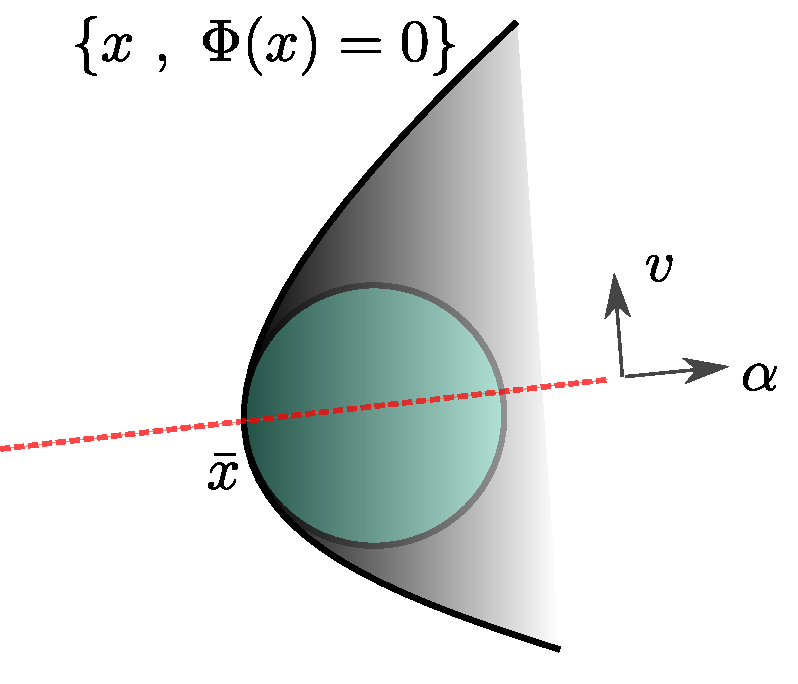
\includegraphics[width=.45\linewidth]{images/constraind_diffusion_rejection/mscxgamma.pdf} \hfill
	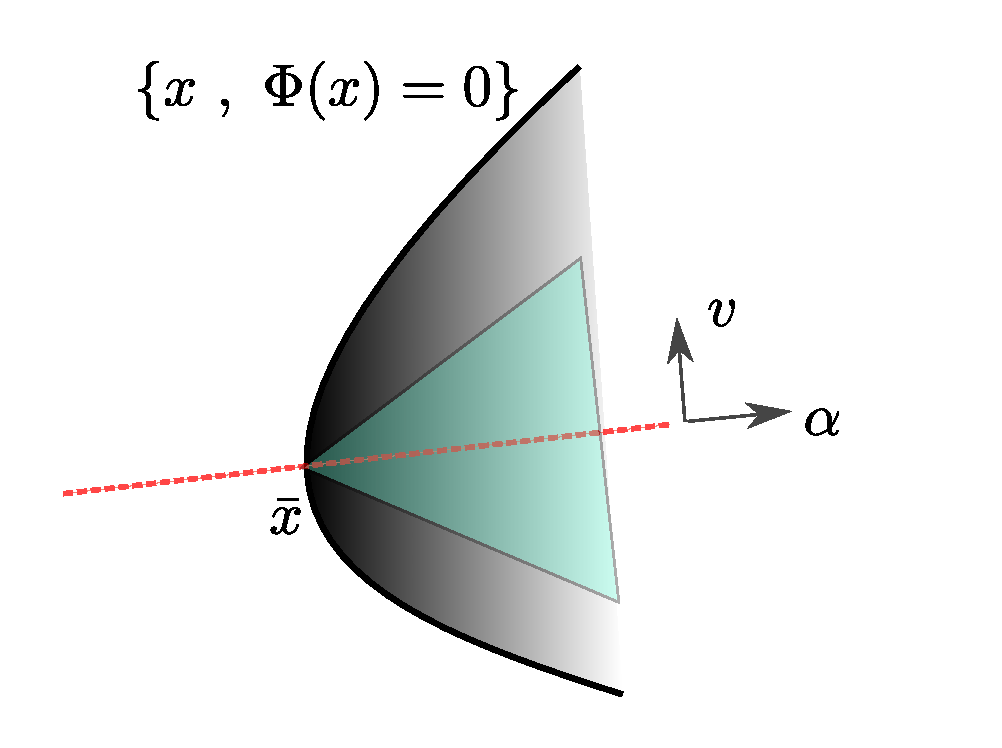
\includegraphics[width=.45\linewidth]{images/constraind_diffusion_rejection/mscxgamma_small.pdf}
	\caption{The grey shaded area represents $\cl{\c{M}}$ while the blue shaded
		area represents $\sf{C}(x, \gamma)$ for an arbitrary value of $\gamma$
		and $x =\bar{x} \in \partial \c{M}$.}
	\label{fig:comparison_area}
\end{figure}

\subsection{Technical lemmas}
\label{sec:technical_lemmas}

We start with a few technical lemmas which will allow us to control some Gaussian probabilities outside of a compact set.
We denote $\Psi: \R_+ \times \N \to \cbr{0,1}$ such that for any $k \in \N$, $\Psi(\cdot, k)$ is the tail probability of a $\chi$-squared random variable with parameter $k$, i.e.~ for any $k \in \N$ and $t \geq 0$ we have \begin{equation} \label{eq:tail_probability} \Psi(t, k) = \bb{P}{\norm{Z}^2 \geq t}, \end{equation} with $Z$ a Gaussian random variable in $\R^k$ with zero mean and identity covariance matrix.
We will make extensive use of the following lemma which is a direct consequence of \cite[Section 4, Lemma 1]{laurent2000adaptive}.

\begin{lemma}
	\label{lemma:tail_chi_square}
	For any $k \in \N$ and $t \in \R_+$ with $t \geq 5k$, $\Psi(t, k) \leq \exp[-t/5]$.
\end{lemma}

\begin{proof}
	Let $k \in \N$.
	First, note that for any $x \geq k$, we have that $k + 2 (k x)^{1/2} + 2x \leq 5x$.
	Combining this result and \cite[Section 4, Lemma 1, Equation (4.3)]{laurent2000adaptive}, we have that for any $x \geq k$ \begin{equation} \bb{P}{\norm{X}^2 \geq 5 x} \leq \exp[-x] , \end{equation} with $X$ a $\R^k$-valued Gaussian random variable with zero mean and identity covariance matrix.
	This concludes the proof upon letting $t = 5x$.
\end{proof}

Let $\varphi: \ \R^p \to \R_+$ given for any $u \in \R$ by $\varphi(u) = (2 \uppi)^{-p/2} \exp[-\norm{u}^2/2]$\footnote{In the rest of the supplementary, we never precise the dimension $p \in \N$ which can be deduced from the variable.
}, i.e.~the density of a real Gaussian random
variable with zero mean and unit variance.
While \Cref{lemma:tail_chi_square_int} appears technical, it will be central to provide quantitative upper bounds on the \emph{rejection} probability, see \Cref{lemma:lower_bound_prob} for instance.

\begin{lemma}
	\label{lemma:tail_chi_square_int}
	For any $k \in \N$, $\alpha_0>0$, $\beta_0 \in \ocbr{0,1}$ and $\delta > 0$ we have \begin{equation} \psi(\delta) = \textstyle{\sup \cbrcolon{\int_0^{+\infty} \Psi(\alpha_0 t/\delta, k)^{\beta_0} \varphi(t - t_0/\delta) \mathrm{d} t}{t_0 \geq 0}} \leq C_0 \delta , \end{equation} with $C_0 = 5(2\uppi)^{-1/2}(k+1)/(\alpha_0 \beta_0)$.
\end{lemma}

\begin{proof}
	Let $k \in \N$, $\alpha_0 >0$, $\beta_0 \in \ocbr{0,1}$ and $\delta > 0$.
	Let $t_{\delta} = 5 k \delta /\alpha_0$.
	Note that if $t \geq t_\delta$ then, $\alpha_0 t /\delta \geq 5k$.
	In addition, we have \begin{align} \textstyle \int_0^{+\infty} \Psi(\alpha_0 t/\delta, k)^{\beta_0} \varphi(t - t_0/\delta) \mathrm{d} t & \textstyle \leq (2 \uppi)^{-1/2} \int_0^{+\infty} \Psi(\alpha_0 t/\delta, k)^{\beta_0} \mathrm{d} t \\ & \textstyle \leq (2 \uppi)^{-1/2} \int_0^{t_\delta} \Psi(\alpha_0 t/\delta, k)^{\beta_0} \mathrm{d} t + (2 \uppi)^{-1/2} \int_{t_\delta}^{+\infty} \Psi(\alpha_0 t/\delta, k)^{\beta_0} \mathrm{d} t .
	\end{align}
	Using that for any $w >0$, $\int_0^{+\infty} \exp[-w t] \mathrm{d} t \leq (1/w)$, that for any $u \geq 0$, $\Psi(u, k) \leq 1$ and that if $u \geq 5k$, $\Psi(u,k) \leq \exp[-u/5]$, we get for any $t_0 \geq 0$ \begin{equation} \textstyle \int_0^{+\infty} \Psi(\alpha_0 t/\delta, k) \varphi(t - t_0/\delta) \leq (2\uppi)^{-1/2} [5k \delta/\alpha_0 + 5 \delta/(\alpha_0 \beta_0)] \leq (5(2\uppi)^{-1/2}(k+1)/(\alpha_0\beta_0)) \delta , \end{equation} which concludes the proof.
\end{proof}

Finally, we have the following lemma, which is similar to \Cref{lemma:tail_chi_square} but will be used to control quantities related to the norm.

\begin{lemma}
	\label{lemma:tail_chi_square_int_duo}
	For any $k \in \N$, $\alpha_0>0$, $\beta_0 \in \ocbr{0,1}$ and $\delta > 0$ we have \begin{equation} \psi(\delta) = \textstyle{ \int_0^{+\infty} \Psi(\alpha_0 t/\delta, k)^{\beta_0} t \varphi(t) \mathrm{d} t} \leq C_0 \delta^2 , \end{equation} with $C_0 = 25(2\uppi)^{-1}(k^2+1)/(\alpha_0\beta_0)^2$.
\end{lemma}

\begin{proof}
	Let $k \in \N$, $\alpha_0 >0$, $\beta_0 \in \ocbr{0,1}$ and $\delta > 0$.
	Let $t_{\delta} = 5 k \delta /\alpha_0$.
	Note that if $t \geq t_\delta$ then, $\alpha_0 t /\delta \geq 5k$.
	In addition, we have \begin{align} \textstyle{ \int_0^{+\infty} \Psi(\alpha_0 t/\delta, k)^{\beta_0} t \varphi(t) \mathrm{d} t} & \leq (2 \uppi)^{-1} \textstyle{ \int_0^{t_\delta} \Psi(\alpha_0 t/\delta, k)^{\beta_0} t \mathrm{d} t} + (2\uppi)^{-1} \textstyle{ \int_{t_\delta}^{+\infty} \Psi(\alpha_0 t/\delta, k)^{\beta_0} t \mathrm{d} t} .
	\end{align}
	In addition, using that if $u \geq 5k$ then $\Psi(u,k) \leq \exp[-u/5]$, we get \begin{align} \textstyle (2\uppi)^{-1} \int_{t_\delta}^{+\infty} \Psi(\alpha_0 t/\delta, k)^{\beta_0} t \mathrm{d} t & \leq (2\uppi)^{-1} \textstyle \int_0^{+\infty} \exp[-\alpha_0\beta_0 t /(5\delta)] t \mathrm{d} t \leq (2\uppi)^{-1} 25 \delta^2 / (\alpha_0 \beta_0)^2 .
	\end{align}
	Finally, using that for any $u \geq 0$, $\Psi(u,k)\leq1$, we have \begin{equation} \textstyle (2 \uppi)^{-1} \textstyle{ \int_0^{t_\delta} \Psi(\alpha_0 t/\delta, k)^{\beta_0} t \mathrm{d} t} \leq (2 \uppi)^{-1} 25 k^2 \delta^2 / \alpha_0^2 , \end{equation} which concludes the proof.
\end{proof}

\subsection{Lower bound on the inside probability and control of moments of order two and higher}
\label{sec:lower_control}

\paragraph{Lower bound on the inside probability.}
We begin with the following lemma which controls the expectation of $1 + \norm{Z}$ \emph{outside} of $\sf{C}(x,\gamma)$.
We recall that $\sf{V}$ is defined in \Cref{thm:tubul-neighb}-\ref{item:c_prime}.

\begin{lemma}
	\label{lemma:control_outside}
	Let $\bar{\gamma} = 1$.
	Let $x \in \sf{V}$, $Z \in \sim \mathrm{N}(0, \m{I})$ and $\gamma \in \del{0, \bar{\gamma}}$ then we have \begin{equation} \max(\E\sbr{\bm{1}_{x + \sqrt{\gamma} Z \in \cl{\c{M}} \cap \sf{C}(x,\gamma)^\mathrm{c}}}, \E\sbr{\langle Z, \nabla \Phi(\bar{x})\rangle \bm{1}_{x + \sqrt{\gamma} Z \in \cl{\c{M}} \cap \sf{C}(x,\gamma)^\mathrm{c}}}) \leq \psi(\gamma) , \end{equation} with $\psi: \ \R_+ \to \R_+$ such that $\limsup_{t \to 0} \psi(t)/t^{1/2} < +\infty$.
\end{lemma}

\begin{proof}

	Let $\bar{r} > 0$ given by \Cref{thm:tubul-neighb}.
	First, we have that \begin{align}  & \textstyle\int_{\R} \int_{\R^{d-1}} (1 + \abs{\alpha} + \norm{v}) \bm{1}_{\alpha \geq \bar{r} /\gamma^{1/2}} \varphi(\alpha) \varphi(v) \mathrm{d} \alpha \mathrm{d} v \\  & \textstyle\qquad \leq d \int_{\R} (1 + \abs{\alpha}) \bm{1}_{\alpha \geq \bar{r} /\gamma^{1/2}} \varphi(\alpha) \mathrm{d} \alpha \leq d (\Psi(\bar{r}^2/\gamma,1) + \exp[-\bar{r}^2/(2\gamma)]) .
                 \label{eq:true_uno}
	\end{align}
	Second, using \Cref{lemma:tail_chi_square_int}, we have that \begin{align}  & \textstyle\int_{\R} \int_{\R^{d-1}}\bm{1}_{\norm{v}^2\geq (\bar{\alpha}+\sqrt{\gamma}\alpha)/(C\gamma)} \bm{1}_{\bar{\alpha}+\sqrt{\gamma}\alpha \geq 0} \varphi(\alpha) \varphi(v) \mathrm{d} \alpha \mathrm{d} v \\ &\qquad \textstyle \leq \int_{\R} \bm{1}_{\bar{\alpha}+\sqrt{\gamma}\alpha \geq 0} \Psi((\bar{\alpha}+\sqrt{\gamma}\alpha)/(C\gamma), d-1) \varphi(\alpha) \mathrm{d} \alpha \\  & \qquad \textstyle \leq \int_{0}^{+\infty} \Psi(\alpha/C\gamma^{1/2}, d-1) \varphi(\alpha-\bar{\alpha}/\gamma^{1/2}) \mathrm{d} \alpha \leq \Psi_1(\gamma^{1/2}) .
                 \label{eq:true_duo}
	\end{align}
	Second, using \Cref{lemma:tail_chi_square_int_duo}, we have that \begin{align}  & \textstyle\int_{\R} \int_{\R^{d-1}}\alpha \bm{1}_{\norm{v}^2\geq (\bar{\alpha}+\sqrt{\gamma}\alpha)/(C\gamma)} \bm{1}_{\bar{\alpha}+\sqrt{\gamma}\alpha \geq 0} \varphi(\alpha) \varphi(v) \mathrm{d} \alpha \mathrm{d} v \\ &\qquad = \textstyle\int_{\R} \alpha \Psi((\bar{\alpha}+\sqrt{\gamma}\alpha)/(C\gamma),d-1) \bm{1}_{\bar{\alpha}+\sqrt{\gamma}\alpha \geq 0} \varphi(\alpha) \mathrm{d} \alpha \\  & \qquad \textstyle \leq \int_0^{+\infty} \Psi(\alpha/C\gamma^{1/2},d-1) \alpha \varphi(\alpha) \mathrm{d} \alpha \leq \Psi_2(\gamma^{1/2}).
                 \label{eq:true_trio}
	\end{align}
	Note that we have $\limsup_{\gamma \to 0} \Psi_2(\gamma^{1/2}) + \Psi_1(\gamma^{1/2}) < +\infty$.
	We conclude upon combining \eqref{eq:true_uno}, \eqref{eq:true_duo} and \eqref{eq:true_trio} with \Cref{thm:tubul-neighb}-\ref{item:d} and the fact that $\norm{\Phi(\bar{x})} =1$.
\end{proof}

The following lemma allow us to give a lower bound to the quantity $\E\sbr{\bm{1}_{x+\sqrt{\gamma}Z \in \cl{\c{M}}}}$ uniformly w.r.t $x \in \cl{\c{M}}$.

\begin{lemma}
	\label{lemma:lower_bound_prob}
	There exists $\bar{\gamma} >0$ such that for any $\gamma \in \del{0, \bar{\gamma}}$ and for any $x \in \cl{\c{M}}$, $\gamma \in \del{0, \bar{\gamma}}$ and $Z \sim \mathrm{N}(0, \m{I})$ we have \begin{equation} \E\sbr{\bm{1}_{x + \sqrt{\gamma} Z \in \cl{\c{M}}}} \geq 1/4 .
	\end{equation}
\end{lemma}

\begin{proof}
	Let $\gamma \in \del{0, \bar{\gamma}}$.
	If $x \not \in \sf{V}$ then $\mathrm{B}(x,2R) \subset \c{M}$ using \Cref{thm:tubul-neighb}-\ref{item:a} and therefore $\E\sbr{\bm{1}_{x + \sqrt{\gamma} Z \in \cl{\c{M}}}} \geq 1/4$ for $\bar{\gamma} > 0$ small enough.
	Now, assume that $x \in \sf{V}$.
	Using \Cref{lemma:control_outside}, we have that $\E\sbr{\bm{1}_{x + \sqrt{\gamma} Z \in \cl{\c{M}}\cap \sf{C}(x, \gamma)^\mathrm{c}}} \leq \psi(\gamma)$.
	In addition, using \Cref{thm:tubul-neighb}-\ref{item:c}, we have that for any $\gamma >0$ \begin{align} \E\sbr{\bm{1}_{x + \sqrt{\gamma} Z \in \cl{\c{M}}}} & \geq \E\sbr{\bm{1}_{x + \sqrt{\gamma} Z \in \sf{C}(x, \gamma)}} \\ &\geq \textstyle{\int_{-\bar{\alpha} \gamma^{-1/2}}^{r \gamma^{-1/2}} \int_{\nabla \Phi(\bar{x})^\perp} \bm{1}_{\norm{v}^2\leq (\bar{\alpha}+\gamma^{1/2}\alpha)/(C\gamma)} \varphi(\alpha)\varphi(v) \mathrm{d} \alpha \mathrm{d} v} \\ &\geq \textstyle{\int_{-\bar{\alpha} \gamma^{-1/2}}^{r \gamma^{-1/2}} (1 - \Psi((\bar{\alpha}+\gamma^{1/2}\alpha)/(C\gamma),d-1)) \varphi(\alpha) \mathrm{d} \alpha} \\  & \textstyle{\geq (1/2) - \Psi(r^2/\gamma, 1) - \int_{-\bar{\alpha} \gamma^{-1/2}}^{+\infty} \Psi((\bar{\alpha}+\gamma^{1/2}\alpha)/(C\gamma),d-1) \varphi(\alpha) \mathrm{d} \alpha.
                 }
	\end{align}
	Hence, using \Cref{lemma:tail_chi_square} and \Cref{lemma:tail_chi_square_int}, there exists $\bar{\gamma} >0$ such that for any $\gamma \in \del{0, \bar{\gamma}}$, $\Psi(r^2/\gamma, 1) + \int_0^{+\infty} \Psi(\alpha/(C\gamma^{1/2}),d) \varphi(\alpha-\gamma^{1/2}\bar{\alpha}) \mathrm{d} \alpha \leq 1/4$, which concludes the proof.
\end{proof}

Note that the result of \Cref{lemma:lower_bound_prob} can be improved to $1/2-\varepsilon$ for any $\varepsilon > 0$.
In particular this result tells us that for $\gamma > 0$ small enough, $\cl{\c{M}}$ looks like the \emph{hyperplane} from the point of view of the Gaussian with variance $\gamma$ centered on $\partial \c{M}$.

\paragraph{Bound on moments of order two and higher.}

In what follows, we define for any $\gamma >0$, $\Delta^\gamma: \ \cl{\c{M}} \to \R_+$ given for any $x \in \cl{\c{M}}$ by \begin{equation} \label{eq:intermediate_Delta} \textstyle{ \Delta^\gamma(x) = (1/\gamma) \int_{\R^d} \bm{1}_{x + \sqrt{\gamma} z \in \c{M}} \norm{\sqrt{\gamma} z}^4 \varphi(z) \mathrm{d} z / \int_{\R^d} \bm{1}_{x + \sqrt{\gamma} z \in \c{M}} \varphi(z) \mathrm{d} z.
	}
\end{equation}

\begin{proposition}
	\label{prop:condition_a}
	We have $\lim_{\gamma \to 0} \sup \cbrcolon{\Delta^\gamma(x)}{x \in \cl{\c{M}}} = 0$.
\end{proposition}

\begin{proof}
	Let $\bar{\gamma} >0$ given by \Cref{lemma:lower_bound_prob}.
	Let $x \in \cl{\c{M}}$ and $\gamma \in \del{0, \bar{\gamma}}$.
	We have using \Cref{lemma:lower_bound_prob} \begin{equation} \textstyle{\int_{\R^d} \bm{1}_{x + \sqrt{\gamma} z \in \c{M}} \varphi(z) \mathrm{d} z \geq 1/4 .
		}
	\end{equation}
	We also have that \begin{equation} \textstyle{ (1/\gamma) \int_{\R^d} \bm{1}_{x + \sqrt{\gamma} z \in \c{M}} \norm{\sqrt{\gamma} z}^4 \varphi(z) \mathrm{d} z \leq 3 \gamma d^2 .
		}
	\end{equation}
	Therefore, we get that for any $\gamma \in \del{0, \bar{\gamma}}$, $\Delta^\gamma(x) \leq 12 \gamma d^2$, which concludes the proof.
\end{proof}

In what follows, we define for any $\gamma >0$, $\hat{\Sigma}^\gamma: \ \cl{\c{M}} \to \mathrm{S}_d^+(\R)$ given for any $x \in \cl{\c{M}}$ by \begin{equation} \label{eq:intermediate_diffusion} \textstyle{ \hat{\Sigma}^\gamma(x) = \int_{\R^d} \bm{1}_{x + \sqrt{\gamma} z \in \c{M}} z \otimes z \varphi(z) \mathrm{d} z / \int_{\R^d} \bm{1}_{x + \sqrt{\gamma} z \in \c{M}} \varphi(z) \mathrm{d} z.
	}
\end{equation}

\begin{proposition}
	\label{prop:condition_d}
	There exists $\bar{\gamma} >0$ such that for any $x \in \cl{\c{M}}$ and $\gamma \in \del{0, \bar{\gamma}}$ we have \begin{equation} \norm{\hat{\Sigma}^\gamma(x)} \leq 4d .
	\end{equation}
\end{proposition}

\begin{proof}
	Let $x \in \cl{\c{M}}$ and $\bar{\gamma} >0$ given by \Cref{lemma:lower_bound_prob}.
	For any $\gamma \in \del{0, \bar{\gamma}}$, we have using \Cref{lemma:lower_bound_prob} \begin{equation} \textstyle{\int_{\R^d} \bm{1}_{x + \sqrt{\gamma} z \in \c{M}} \varphi(z) \mathrm{d} z \geq 1/4 .
		}
	\end{equation}
	We also have that \begin{equation} \textstyle{ \int_{\R^d} \bm{1}_{x + \sqrt{\gamma} z \in \c{M}} \norm{z}^2 \varphi(z) \mathrm{d} z \leq d , } \end{equation} which concludes the proof.
\end{proof}

\subsection{Properties of large drift terms}
\label{sec:large_drift_properties}

Finally, we define for any $\gamma >0$, $\hat{b}^\gamma: \ \cl{\c{M}} \to \R^d$ given for any $x \in \cl{\c{M}}$ by \begin{equation} \label{eq:intermediate_drift} \textstyle{ \hat{b}^\gamma(x) = \gamma^{-1/2} \int_{\R^d} \bm{1}_{x + \sqrt{\gamma} z \in \c{M}} z \varphi(z) \mathrm{d} z / \int_{\R^d} \bm{1}_{x + \sqrt{\gamma} z \in \c{M}} \varphi(z) \mathrm{d} z.
	}
\end{equation}
First, we show away from the boundary the drift $\hat{b}^\gamma$ converges to zero.

\begin{proposition}
	\label{prop:away_implies_small}
	There exists $\bar{\gamma} >0$ such that for any $\gamma \in \del{0, \bar{\gamma}}$, $r > 0$ and $x \in \cl{\c{M}}$ such that $d(x, \partial \c{M}) \geq r$ we have $\norm{\hat{b}^\gamma(x)} \leq 2d \Psi(r/\gamma,d)^{1/2}/\gamma^{1/2}$.
\end{proposition}

\begin{proof}
	Let $x \in \cl{\c{M}}$ and $\bar{\gamma} >0$ given by \Cref{lemma:lower_bound_prob}.
	For any $\gamma \in \del{0, \bar{\gamma}}$ we have using \Cref{lemma:lower_bound_prob} \begin{equation} \textstyle{\int_{\R^d} \bm{1}_{x + \sqrt{\gamma} z \in \c{M}} \varphi(z) \mathrm{d} z \geq 1/4 .
		}
	\end{equation}
	We also have that \begin{align} \textstyle{\norm{\int_{\R^d} \bm{1}_{x + \sqrt{\gamma} z \in \c{M}} z \varphi(z) \mathrm{d} z}} &\leq \textstyle{\norm{\int_{\R^d} \bm{1}_{\norm{z} \leq r/\gamma^{1/2}} z \varphi(z) \mathrm{d} z}} + \int_{\R^d} \bm{1}_{\norm{z} \geq r/\gamma^{1/2}} \norm{z} \varphi(z) \mathrm{d} z \\ &\leq \textstyle{2 \int_{\R^d} \bm{1}_{\norm{z} \geq r/\gamma^{1/2}} \norm{z} \varphi(z) \mathrm{d} z} \leq 2d \Psi(r/\gamma,d)^{1/2}/\gamma^{1/2} , \end{align} which concludes the proof.
\end{proof}

We have the following corollary.
\begin{corollary}
	\label{coro:condition_c}
	There exists $\bar{\gamma} >0$ such that for any $\delta >0$ there exists $M_\delta >0$ such that for any $\gamma \in \del{0, \bar{\gamma}}$ and $x \in \cl{\c{M}}$, $\norm{\hat{b}^\gamma(x)} \geq M_\delta$, then $\Phi(x) \leq \delta$.
\end{corollary}

\begin{proof}
	Let $\bar{\gamma} >0$ given by \Cref{lemma:lower_bound_prob}.
	Let $f: \ \R_+ \to \R_+$ given for any $r > 0$ by $f(r) = \sup \cbrcolon{\gamma > 0}{\Psi(r/\gamma,1)^{1/2}/\gamma^{1/2}}$.
	We have that $f$ is non-increasing and $\lim_{r \to 0} f(r)=+\infty$.
	Let $\delta > 0$ and $M_\delta =2df(\delta/C)$ with $C = \sup \cbrcolon{\norm{\nabla \Phi(x)}}{x \in \cl{\c{M}}}$.
	Let $\gamma \in \del{0, \bar{\gamma}}$ and $x \in \cl{\c{M}}$ such that $\norm{\hat{b}^\gamma(x)} \geq M_\delta$ then using \Cref{prop:away_implies_small} we have that $d(x, \partial \c{M}) \leq \delta / C$.
	Let $\bar{x} \in \partial \c{M}$ such that $\norm{x - \bar{x}} = d(x, \partial \c{M})$.
	We have \begin{equation} \textstyle{\Phi(x) \leq \Phi(\bar{x}) + \int_0^1 \langle \nabla \Phi(\bar{x} + t(x-\bar{x})), x - \bar{x} \rangle \mathrm{d} t \leq \delta,} \end{equation} which concludes the proof.
\end{proof}

For ease of notation, for any $\gamma >0$, we define $\bar{b}^\gamma = \gamma^{1/2} \hat{b}^\gamma$, the \emph{renormalized} version of the drift.
First, we have the following result which will ensure that the drift projected on the normal component does not vanish.

\begin{lemma}
	\label{lemma:complement_computation}
	There exists $\bar{\gamma} > 0$ such that for any $\gamma \in \del{0, \bar{\gamma}}$ and $x \in \sf{V}$ we have \begin{equation} \langle \bar{b}^\gamma(x), \nabla \Phi(\bar{x}) \rangle \geq \norm{\bar{b}^\gamma(x)} - \psi(\gamma) , \end{equation} with $\psi: \ \R_+ \to \R_+$ such that $\limsup_{\gamma \to 0} \psi(\gamma)/\sqrt{\gamma} <+\infty$.
\end{lemma}

\begin{proof}
	Let $x \in \cl{\c{M}}$ and $\bar{\gamma} >0$ given by \Cref{lemma:lower_bound_prob}.
	For any $\gamma \in \del{0, \bar{\gamma}}$ we have using \Cref{lemma:lower_bound_prob} \begin{equation} \label{eq:lowr} \textstyle{\int_{\R^d} \bm{1}_{x + \sqrt{\gamma} z \in \c{M}} \varphi(z) \mathrm{d} z \geq 1/4 .
		}
	\end{equation}
	In addition, we have \begin{align} \textstyle{\int_{\R^d} \bm{1}_{x + \sqrt{\gamma}z \in \c{M}} \langle z, \nabla \Phi(\bar{x}) \rangle \varphi(z) \mathrm{d} z} & \geq \textstyle{ \int_{\R^d} \bm{1}_{x + \sqrt{\gamma}z \in \sf{C}(x,\gamma)} \langle z, \nabla \Phi(\bar{x}) \rangle \varphi(z) \mathrm{d} z} \\ & \qquad \textstyle{-\int_{\R^d} \bm{1}_{x + \sqrt{\gamma}z \in \c{M} \cap \sf{C}(x,\gamma)^\mathrm{c}} \langle z, \nabla \Phi(\bar{x}) \rangle \varphi(z) }.
	\end{align}
	Using \Cref{lemma:control_outside}, we get that \begin{equation} \label{eq:ineq_remove} \textstyle{\int_{\R^d} \bm{1}_{x + \sqrt{\gamma}z \in \c{M}} \langle z, \nabla \Phi(\bar{x}) \rangle \varphi(z) \mathrm{d} z} \geq \textstyle{ \int_{\R^d} \bm{1}_{x + \sqrt{\gamma}z \in \sf{C}(x,\gamma)} \langle z, \nabla \Phi(\bar{x}) \rangle \varphi(z) \mathrm{d} z} - \psi(\gamma) .
	\end{equation}
	Let $\{e_i \}_{i=1}^{d-1}$ a basis of $\nabla \Phi(\bar{x})^\perp$.
	Using \Cref{thm:tubul-neighb}-\ref{item:c}, we have that for any $i \in \{1, \dots, d-1\}$ \begin{align} \textstyle{ \int_{\R^d} \bm{1}_{x + \sqrt{\gamma}z \in \sf{C}(x,\gamma)} \langle z, e_i \rangle \varphi(z) \mathrm{d} z} & \textstyle{= \int_{-\bar{\alpha}/\gamma^{1/2}}^{r/\gamma^{1/2}} \int_{\nabla \Phi(\bar{x})^\perp} \bm{1}_{\norm{v}^2 \leq (\gamma^{1/2} \alpha + \bar{\alpha})/\gamma} \langle v, e_i \rangle \varphi(v) \varphi(\alpha) \mathrm{d} v \mathrm{d} \alpha}.
	\end{align}
	Hence, combining this result and the Cauchy-Schwarz inequality we have for any $i \in \{1, \dots, d-1\}$ \begin{align} \textstyle & \textstyle (\int_{\R^d} \bm{1}_{x + \sqrt{\gamma}z \in \sf{C}(x,\gamma)} \langle z, e_i \rangle \varphi(z) \mathrm{d} z)^2 = \textstyle (\int_{-\bar{\alpha}/\gamma^{1/2}}^{r/\gamma^{1/2}} \int_{\nabla \Phi(\bar{x})^\perp} \bm{1}_{\norm{v}^2 \geq (\gamma^{1/2} \alpha + \bar{\alpha})/\gamma} \langle v, e_i \rangle \varphi(v) \varphi(\alpha) \mathrm{d} v \mathrm{d} \alpha)^2 \\ &\qquad \qquad \leq \textstyle \int_{\nabla \Phi(\bar{x})^\perp} \langle v, e_i \rangle^2 \varphi(v) \mathrm{d} v (\int_{-\bar{\alpha}/\gamma^{1/2}}^{r/\gamma^{1/2}} \Psi((\bar{\alpha} + \alpha\gamma^{1/2})/\gamma, d-1)^{1/2} \varphi(\alpha) \mathrm{d} \alpha )^2 \\ &\qquad \qquad \textstyle \leq (\int_{-\bar{\alpha}/\gamma^{1/2}}^{r/\gamma^{1/2}} \Psi((\bar{\alpha} + \alpha\gamma^{1/2})/\gamma, d-1)^{1/2} \varphi(\alpha) \mathrm{d} \alpha )^2 .
	\end{align}
	Hence, using \Cref{lemma:tail_chi_square_int}, we get that \begin{equation} \textstyle{\sum_{i=1}^{d-1}( \int_{\R^d} \bm{1}_{x + \sqrt{\gamma}z \in \sf{C}(x,\gamma)} \langle z, e_i \rangle \varphi(z) \mathrm{d} z)^2} \leq (d-1) \psi^2(\gamma) , \end{equation} with $\psi$ given by \Cref{lemma:tail_chi_square_int} with $\beta_0=1/2$.
	Therefore, we get that \begin{align}  & \textstyle{(\int_{\R^d} \bm{1}_{x + \sqrt{\gamma}z \in \sf{C}(x,\gamma)} \langle z, \nabla \Phi(\bar{z}) \rangle \varphi(z) \mathrm{d} z)^2} \\ &\qquad = \textstyle (\int_{\R^d} \bm{1}_{x + \sqrt{\gamma} z \in \c{M}} \varphi(z) \mathrm{d} z)^2 \textstyle{\norm{\bar{b}^\gamma(x)}^2 - \sum_{i=1}^{d-1}( \int_{\R^d} \bm{1}_{x + \sqrt{\gamma}z \in \sf{C}(x,\gamma)} \langle z, e_i \rangle \varphi(z) \mathrm{d} z)^2} \\ &\qquad \geq \textstyle (\int_{\R^d} \bm{1}_{x + \sqrt{\gamma} z \in \c{M}} \varphi(z) \mathrm{d} z)^2 \norm{\bar{b}^\gamma(x)}^2 - \psi(\gamma)^2.
	\end{align}
	We conclude the proof upon using that for any $a,b \geq 0$, $(a+b)^{1/2} \leq a^{1/2} + b^{1/2}$ and \eqref{eq:lowr}.
\end{proof}

We are now ready to state the following lower bound on the drift.

\begin{proposition}
	\label{prop:lower-bound-drift}
	There exist $\bar{\gamma} >0$, $M \geq 0$ and $c >0$ such that for any $x \in \cl{\c{M}}$ and $\gamma \in \del{0, \bar{\gamma}}$ if $\norm{\hat{b}^\gamma(x)} \geq M$ then $x \in \sf{V}$ and \begin{equation} \min(\langle \hat{b}^\gamma(x), \nabla \Phi(x) \rangle, \langle \hat{b}^\gamma(x), \nabla \Phi(\bar{x}) \rangle) \geq c \norm{\hat{b}^\gamma(x)} .
	\end{equation}
\end{proposition}

\begin{proof}
	Let $\bar{\gamma} >0$ given by \Cref{lemma:lower_bound_prob} and $M_0 = 4 \sup \cbrcolon{\psi(\gamma)/\gamma^{1/2}}{\gamma \in \ocbr{0, \bar{\gamma}}}$.
	In addition, let $c = 1/4$.
	Using \Cref{prop:away_implies_small} and \Cref{thm:tubul-neighb}-\ref{item:a}, there exists $M_1 \geq 0$ such that for any any $x \in \cl{\c{M}}$, if $\norm{\hat{b}^\gamma(x)} \geq M_1$ then $x \in \sf{V}$ and $x = \bar{x} + \alpha \nabla \Phi(\bar{x})$ with $\alpha \leq 1/(4C)$ and $C = \sup \cbrcolon{\norm{\nabla^2 \Phi(x)}}{x \in \cl{\c{M}}}$.
	We denote $M = \max(M_0, M_1)$.
	Let $\gamma \in \del{0, \bar{\gamma}}$ and $x \in \cl{\c{M}}$ such that $\norm{\hat{b}^\gamma(x)} \geq M$.
	Using \Cref{lemma:complement_computation}, we have that \begin{equation} \langle \hat{b}^\gamma(x), \nabla \Phi(\bar{x}) \rangle \geq \norm{\hat{b}^\gamma(x)} - \psi(\gamma)/\gamma^{1/2} .
	\end{equation}
	Using that $\psi(\gamma)/\gamma^{1/2} \leq M/2 \leq \norm{\hat{b}^\gamma(x)}/2$, we have \begin{equation} \langle \hat{b}^\gamma(x), \nabla \Phi(\bar{x}) \rangle \geq (1/2) \norm{\hat{b}^\gamma(x)} .
	\end{equation}
	Since $\norm{x - \bar{x}} \leq \alpha \leq 1/(4C)$ we have $\langle \hat{b}^\gamma(x), \nabla \Phi(x) \rangle \geq (1/2 - C \alpha ) \norm{\hat{b}^\gamma(x)} \geq \norm{\hat{b}^\gamma(x)} / 4$, which concludes the proof.
\end{proof}

\subsection{Convergence on compact sets}
\label{sec:convergence_on_compact}

In this section, we show the convergence of the drift and diffusion matrix on compact sets.
We recall that $\c{M}$ does \emph{not} include its boundary $\partial \c{M}$.

\begin{proposition}
	\label{prop:condition_uno}
	For any compact set $\sf{K} \subset \c{M}$ and $\varepsilon >0$, there exists $\bar{\gamma} >0$ such that for any $\gamma \in \del{0, \bar{\gamma}}$ we have for any $x \in \sf{K}$ \begin{equation} \norm{\hat{b}^\gamma(x)} \leq \varepsilon , \qquad \norm{\hat{\Sigma}^\gamma(x) - \m{I}} \leq \varepsilon .
	\end{equation}
\end{proposition}

\begin{proof}
	Let $\sf{K} \subset \c{M}$ be a compact set and $\gamma >0$.
	Since $\sf{K} \cap \partial \c{M} = \emptyset$, there exists $r > 0$ such that for any $x \in \sf{K}$, $d(x, \partial \c{M}) > r$.
	Therefore, we have that for any $x \in \sf{K}$ \begin{equation} \textstyle{ \norm{\hat{b}^\gamma(x)} = \gamma^{-1/2} \norm{\int_{x + \sqrt{\gamma}z \in \c{M}} z \varphi(z) \mathrm{d} z} / \int_{x + \sqrt{\gamma}z \in \c{M}} \varphi(z) \mathrm{d} z .
		}
	\end{equation}
	In addition, using the Cauchy-Schwarz inequality we have \begin{align} \textstyle{\norm{\int_{x + \sqrt{\gamma}z \in \c{M}} z \varphi(z) \mathrm{d} z}} & \leq \norm{ \textstyle{\int_{\R^d} z \varphi(z) \mathrm{d} z}} + \int_{\c{M}^\mathrm{c}} \norm{z} \varphi(z) \mathrm{d} z \\  & \leq \textstyle{\int_{\R^d} \bm{1}_{\norm{z} \geq r / \gamma^{1/2}} \norm{z} \varphi(z) \mathrm{d} z \leq \sqrt{d} \Psi(r^2/\gamma, d)^{1/2} .
                 }
	\end{align}
	Using \Cref{lemma:tail_chi_square} and \Cref{lemma:lower_bound_prob}, there exists $\bar{\gamma}_0 >0$ such that for any $\gamma \in \del{0, \bar{\gamma}_0}$ we have that for any $x \in \sf{K}$ \begin{equation} \norm{\hat{b}^\gamma(x)} \leq 4d\Psi(r^2/\gamma,1)^{1/2}/\gamma^{1/2} \leq \varepsilon , \end{equation} which concludes the first part of the proof.
	Similarly, we have that for any $x \in \sf{K}$ \begin{align} \textstyle{\norm{\int_{x + \sqrt{\gamma}z \in \c{M}} (z \otimes z - \m{I}) \varphi(z) \mathrm{d} z}} & \leq \norm{ \textstyle{\int_{\R^d} (z\otimes z - \m{I}) \varphi(z) \mathrm{d} z}} + \int_{\c{M}^\mathrm{c}} \norm{z} \varphi(z) \mathrm{d} z \\ &\leq \textstyle{\int_{\R^d} \bm{1}_{\norm{z} \geq r / \gamma^{1/2}} \norm{z \otimes z - \m{I}} \varphi(z) \mathrm{d} z} \\ & \leq \sqrt{2}(1 + 3d^2)^{1/2} \Psi(r^2/\gamma, d)^{1/2} .
	\end{align}
	Using \Cref{lemma:tail_chi_square} and \Cref{lemma:lower_bound_prob}, there exists $\bar{\gamma}_1 >0$ such that for any $\gamma \in \del{0, \bar{\gamma}_1}$, we have that for any $x \in \sf{K}$ \begin{equation} \norm{\hat{\Sigma}^\gamma(x) - \m{I}} \leq 4 \sqrt{2}(1 + 3d^2)^{1/2} \Psi(r^2/\gamma, 1)^{1/2} \leq \varepsilon , \end{equation} which concludes the proof upon letting $\bar{\gamma} = \min(\bar{\gamma}_0, \bar{\gamma}_1)$.
\end{proof}

\subsection{Convergence on the boundary}
\label{sec:convergence_boundary}

Finally, we investigate the behavior at the boundary of the diffusion matrix and the drift.
First, we show that there is a lower bound to the diffusion matrix near the boundary.
Second, we show that the renormalized drift converges to the outward normal.

\begin{proposition}
	\label{prop:condition_duo_iii}
	There exist $c > 0$ and $\bar{\gamma} >0$ such that for any $\gamma \in \del{0, \bar{\gamma}}$, $u \in \R^d$ and $x \in \sf{V}$ we have \begin{equation} \label{eq:lower_bound_diffusion} \langle u, \hat{\Sigma}^\gamma(x) u \rangle \geq c \norm{u}^2 .
	\end{equation}
	In particular, there exist $r, \varepsilon >0$ such that for any $\gamma \in \del{0, \bar{\gamma}}$ and $x \in \cl{\c{M}}$ with $d(x, \partial \c{M}) \leq r$ \begin{equation} \label{eq:lower_boundary} \langle \nabla \Phi(x), \hat{\Sigma}^\gamma(x) \nabla \Phi(x) \rangle \geq \varepsilon .
	\end{equation}
\end{proposition}

\begin{proof}
	First, we show \eqref{eq:lower_bound_diffusion}.
	Let $x \in \sf{V}$.
	We have for any $u \in \R^d$ \begin{align} \label{eq:first-lower} \langle u, \hat{\Sigma}^\gamma(x) u \rangle & = \textstyle{\int_{\R^d} \bm{1}_{x +\sqrt{\gamma}z \in \c{M}} \langle z, u\rangle^2 \varphi(z) \mathrm{d} z / \int_{\R^d} \bm{1}_{x +\sqrt{\gamma}z \in \c{M}} \mathrm{d} z } \\ &\geq \textstyle{\int_{\R^d} \bm{1}_{x+\sqrt{\gamma} z \in \sf{C}(x,\gamma)} \langle z, u\rangle^2 \varphi(z) \mathrm{d} z} .
	\end{align}
	For any $u \in \R^d$, let $\alpha_u = \langle u, \nabla \Phi(\bar{x}) \rangle$.
	Using \Cref{thm:tubul-neighb}-\ref{item:c} we have for any $u \in \R^d$ \begin{align}  & \textstyle \int_{\R^d} \bm{1}_{x+\sqrt{\gamma} z \in \sf{C}(x,\gamma)} \langle z, u\rangle^2 \varphi(z) \mathrm{d} z \\ &\qquad \textstyle = \int_{-\bar{\alpha}/\gamma^{1/2}}^{r/\gamma^{1/2}} \int_{\nabla \Phi(\bar{x})^\perp} (\langle u, v \rangle + \alpha \alpha_u)^2 \bm{1}_{\norm{v}^2 \leq (\alpha \gamma^{1/2} + \bar{\alpha})/\gamma} \varphi(v) \varphi(\alpha) \mathrm{d} v \mathrm{d} \alpha \\ &\qquad \qquad \textstyle \geq \int_{0}^{r/\gamma^{1/2}} \int_{\nabla \Phi(\bar{x})^\perp} (\langle u, v \rangle^2 + \alpha^2 \alpha_u^2) \bm{1}_{\norm{v}^2 \leq (\alpha \gamma^{1/2} + \bar{\alpha})/\gamma} \varphi(v) \varphi(\alpha) \mathrm{d} v \mathrm{d} \alpha \\  & \qquad \qquad\textstyle \geq \alpha_u^2 \int_0^{r/\gamma^{1/2}} \alpha^2 \varphi(\alpha) \mathrm{d} \alpha + \int_{-\bar{\alpha}/\gamma^{1/2}}^{r/\gamma^{1/2}} \int_{\nabla \Phi(\bar{x})^\perp} \langle u, v \rangle^2 \bm{1}_{\norm{v}^2 \leq (\alpha \gamma^{1/2} + \bar{\alpha})/\gamma} \varphi(v) \varphi(\alpha) \mathrm{d} v \mathrm{d} \alpha .
                 \label{eq:lower_bound_decomp}
	\end{align}
	Using Cauchy-Schwarz inequality, we have \begin{equation} \label{eq:lower_bound_easy} \textstyle\int_0^{r/\gamma^{1/2}} \alpha^2 \varphi(\alpha) \mathrm{d} \alpha = (1/2) - \int_{r/\gamma^{1/2}}^{+\infty} \alpha^2 \varphi(\alpha) \mathrm{d} \alpha \geq (1/2) - 3 \Phi(r^2/\gamma,1)^{1/2}.
	\end{equation}
	In addition, using the Cauchy-Schwarz inequality, we have that \begin{align}  & \textstyle \int_{-\bar{\alpha}/\gamma^{1/2}}^{r/\gamma^{1/2}} \int_{\nabla \Phi(\bar{x})^\perp} \langle u, v \rangle^2 \bm{1}_{\norm{v}^2 \leq (\alpha \gamma^{1/2} + \bar{\alpha})/\gamma} \varphi(v) \varphi(\alpha) \mathrm{d} v \mathrm{d} \alpha \\ & \qquad \qquad \qquad = \textstyle \int_{\nabla \Phi(\bar{x})^\perp} \langle u, v \rangle^2 \varphi(v) \mathrm{d} v \int_{-\bar{\alpha}/\gamma^{1/2}}^{r/\gamma^{1/2}} \varphi(\alpha) \mathrm{d} \alpha \\ &\qquad \qquad \qquad \qquad \qquad \qquad \qquad \textstyle - \int_{-\bar{\alpha}/\gamma^{1/2}}^{r/\gamma^{1/2}} \int_{\nabla \Phi(\bar{x})^\perp} \langle u, v \rangle^2 \bm{1}_{\norm{v}^2 \geq (\alpha \gamma^{1/2} + \bar{\alpha})/\gamma} \varphi(v) \varphi(\alpha) \mathrm{d} v \mathrm{d} \alpha \\ & \qquad \geq \textstyle (\norm{u}^2 - \alpha_u^2) ((1/2) - \Phi(r^2/\gamma,1)) \\ & \qquad \qquad \textstyle - \sqrt{3}(d-1) \norm{u}^2 \int_0^{+\infty} \Phi(\alpha/\gamma^{1/2},d-1)^{1/2} \varphi(\alpha - \bar{\alpha}/\gamma^{1/2}) \mathrm{d} \alpha .
	\end{align}
	Combining this result, \eqref{eq:lower_bound_easy}, \eqref{eq:lower_bound_decomp} and \Cref{lemma:tail_chi_square_int} there exists $\bar{\gamma} > 0$ such that for any $\gamma \in \ocbr{0, \bar{\gamma}}$ and $ u \in \R^d$ \begin{equation} \label{eq:inter_lower_sigma} \textstyle{\int_{\R^d} \bm{1}_{x+\sqrt{\gamma} z \in \sf{C}(x,\gamma)} \langle z, u\rangle^2 \varphi(z) \mathrm{d} z} \geq (1/4) \norm{u}^2 , \end{equation} which concludes the proof of \eqref{eq:lower_bound_diffusion}.
	Finally, using \Cref{thm:tubul-neighb}-\ref{item:a}, we have that for any $x \in \cl{\c{M}}$ if $d(x, \partial \c{M}) \leq R$ then $x \in \sf{V}$.
	Let $r = \min(R, 1/(2C))$ with $C = \sup \cbrcolon{\norm{\nabla^2 \Phi(x)}}{x \in \cl{\c{M}}}$.
	We have that for any $x \in \cl{\c{M}}$ such that $d(x, \partial \c{M})\leq r$ \begin{equation} \norm{\nabla \Phi(x)} \geq \norm{\nabla \Phi(\bar{x}_0)} - C r \geq 1/2 , \end{equation} where $\bar{x}_0$ is such that $\norm{x - \bar{x}_0} \leq r$ and $\bar{x}_0 \in \partial \c{M}$.
	Combining this result and \eqref{eq:inter_lower_sigma} concludes the proof upon letting $\varepsilon = 1/16$.
\end{proof}

Finally, we investigate the behavior of the normalized drift near the boundary.

\begin{proposition}
	\label{prop:condition_duo_iv}
	For any $\bar{x}_0 \in \partial \c{M}$ and $\varepsilon >0$, there exist $\bar{\gamma}, r, M >0$ such that for any $x \in \cl{\c{M}}$ and $\gamma \in \del{0, \bar{\gamma}}$ with $\norm{x - \bar{x}_0} \leq r$ and $\norm{\hat{b}^\gamma(x)} \geq M$ \begin{equation} \norm{\hat{b}^\gamma(x)/\langle \hat{b}^\gamma(x), \nabla \Phi(x) \rangle - \nabla \Phi(\bar{x}_0)} \leq \varepsilon .
	\end{equation}
\end{proposition}

\begin{proof}
	Let $\bar{\gamma}$ be given by \Cref{prop:lower-bound-drift}.
	Let $\psi$ given by \Cref{lemma:tail_chi_square_int} and $M_0 = \sup \cbrcolon{\psi(\gamma)/\gamma^{1/2}}{\gamma \in \del{0, \bar{\gamma}}} < +\infty$.
	Let $M = 16 M_0 / (c\varepsilon^{1/2})$ with $c$ given in \Cref{prop:lower-bound-drift}.
	Let $R > 0$ given by \Cref{thm:tubul-neighb}-\ref{item:a} such that for any $x \in \cl{\c{M}}$ with $d(x, \partial \c{M})$ there exist $\bar{x} \in \partial \c{M}$ and $\alpha \in \cbr{0, c \varepsilon /(4C)}$ such that $x = \bar{x} + \alpha \nabla \Phi(\bar{x})$ with $C = \sup \cbrcolon{\norm{\nabla^2 \Phi(x)}}{x \in \cl{\c{M}}}$ and $c$ given in \Cref{prop:lower-bound-drift}.
	Let $r = \min(\bar{r}, c \varepsilon/4, R)$ and $x \in \cl{M}$ with $\norm{x - \bar{x}_0} \leq r$.
	First, since $d(x, \partial \c{M}) \leq R$, there exist $\bar{x} \in \partial \c{M}$ and $\alpha \in \cbr{0,\varepsilon/(4C)}$ such that $x = \bar{x} + \alpha \nabla \Phi(\bar{x})$.
	Therefore, we get that $\norm{\bar{x} - \bar{x}_0} \leq \varepsilon/(2C)$ and therefore $\norm{\nabla \Phi(\bar{x}_0) - \nabla \Phi(\bar{x})} \leq \varepsilon /2$.
	In addition, we have that \begin{align}  & \norm{\hat{b}^\gamma(x)/\langle \hat{b}^\gamma(x), \nabla \Phi(x) \rangle - \hat{b}^\gamma(x)/\langle \hat{b}^\gamma(x), \nabla \Phi(\bar{x}) \rangle} \\ & \qquad \qquad \leq \norm{\hat{b}^\gamma(x)}^2 \norm{\nabla \Phi(x) - \nabla \Phi(\bar{x})} / (\langle \hat{b}^\gamma(x), \nabla \Phi(x) \rangle \langle \hat{b}^\gamma(x), \nabla \Phi(\bar{x}) \rangle) .
	\end{align}
	Using \Cref{prop:lower-bound-drift}, we get that \begin{equation} \norm{\hat{b}^\gamma(x)/\langle \hat{b}^\gamma(x), \nabla \Phi(x) \rangle - \hat{b}^\gamma(x)/\langle \hat{b}^\gamma(x), \nabla \Phi(\bar{x}) \rangle} \leq \varepsilon/4 .
	\end{equation}
	In what follows, we show that \begin{equation} \norm{\hat{b}^\gamma(x)/\langle \hat{b}^\gamma(x), \nabla \Phi(\bar{x}) \rangle - \nabla \Phi(\bar{x})}^2 \leq \varepsilon/2 .
	\end{equation}
	In particular, we show that for any $u \in \nabla \Phi(\bar{x})^\perp$ with $\norm{u}=1$, \begin{equation} \label{eq:ineq_b_gamma} \langle \hat{b}^\gamma(x), u \rangle ^2 \leq (\varepsilon/16) \langle \hat{b}^\gamma(x), \nabla \Phi(\bar{x}) \rangle^2.
	\end{equation}
	Assuming \eqref{eq:ineq_b_gamma}, letting $u = (\hat{b}^\gamma(x) - \langle \hat{b}^\gamma(x), \nabla \Phi(\bar{x} \rangle)) / (\norm{\hat{b}^\gamma(x)}^2 - \langle \hat{b}^\gamma(x), \nabla \Phi(\bar{x} \rangle^2)^{1/2}$ and using that $\hat{b}^\gamma(x) = \langle \hat{b}^\gamma(x), u\rangle u + \langle \hat{b}^\gamma(x), \nabla \Phi(\bar{x}) \rangle \nabla \Phi(\bar{x})$ we have \begin{align} \norm{\hat{b}^\gamma(x) / \langle \hat{b}^\gamma(x), \nabla \Phi(x) \rangle - \nabla \Phi(\bar{x})} &\leq \norm{\hat{b}^\gamma(x) / \langle \hat{b}^\gamma(x), \nabla \Phi(\bar{x}) \rangle - \nabla \Phi(\bar{x})} \\ & \qquad + \norm{\hat{b}^\gamma(x) / \langle \hat{b}^\gamma(x), \nabla \Phi(x) \rangle - \hat{b}^\gamma(x) / \langle \hat{b}^\gamma(x), \nabla \Phi(\bar{x})\rangle} \\ &\leq \abs{\langle \hat{b}^\gamma(x), u\rangle / \langle \hat{b}^\gamma(x), \nabla \Phi(\bar{x}) \rangle} + \varepsilon / 4 \leq \varepsilon / 2 , \end{align} which concludes the proof.
	Let $u \in \nabla \Phi(\bar{x})^\perp$ with $\norm{u}=1$ and $\{e_i \}_{i=1}^{d-1}$ an orthonormal basis of $\nabla \Phi(\bar{x})^\perp$.
	There exist $\{a_i\}_{i=1}^{d-1}$ such that $\sum_{i=1}^{d-1} a_i^2 = 1$ and $u = \sum_{i=1}^{d-1} a_i e_i$.
	Using \Cref{thm:tubul-neighb}-\ref{item:c}, we have that for any $i \in \{1, \dots, d-1\}$ \begin{align} \textstyle{ \int_{\R^d} \bm{1}_{x + \sqrt{\gamma}z \in \sf{C}(x,\gamma)} \langle z, e_i \rangle \varphi(z) \mathrm{d} z}&\textstyle{= \int_{-\bar{\alpha}/\gamma^{1/2}}^{r/\gamma^{1/2}} \int_{\nabla \Phi(\bar{x})^\perp} \bm{1}_{\norm{v}^2 \leq (\gamma^{1/2} \alpha + \bar{\alpha})/\gamma} \langle v, e_i \rangle \varphi(v) \varphi(\alpha) \mathrm{d} v \mathrm{d} \alpha} \\ &= \textstyle{\int_{-\bar{\alpha}/\gamma^{1/2}}^{r/\gamma^{1/2}} \int_{\nabla \Phi(\bar{x})^\perp} \bm{1}_{\norm{v}^2 \geq (\gamma^{1/2} \alpha + \bar{\alpha})/\gamma} \langle v, e_i \rangle \varphi(v) \varphi(\alpha) \mathrm{d} v \mathrm{d} \alpha}\end{align} Hence, combining this result and the Cauchy-Schwarz inequality we have for any $i \in \{1, \dots, d-1\}$ \begin{align}  & \textstyle (\int_{\R^d} \bm{1}_{x + \sqrt{\gamma}z \in \sf{C}(x,\gamma)} \langle z, e_i \rangle \varphi(z) \mathrm{d} z)^2 = \textstyle (\int_{-\bar{\alpha}/\gamma^{1/2}}^{r/\gamma^{1/2}} \int_{\nabla \Phi(\bar{x})^\perp} \bm{1}_{\norm{v}^2 \geq (\gamma^{1/2} \alpha + \bar{\alpha})/\gamma} \langle v, e_i \rangle \varphi(v) \varphi(\alpha) \mathrm{d} v \mathrm{d} \alpha)^2 \\ & \qquad \leq \textstyle \int_{\nabla \Phi(\bar{x})^\perp} \langle v, e_i \rangle^2 \varphi(v) \mathrm{d} v (\int_{-\bar{\alpha}/\gamma^{1/2}}^{r/\gamma^{1/2}} \Psi((\bar{\alpha} + \alpha\gamma^{1/2})/\gamma, d-1)^{1/2} \varphi(\alpha) \mathrm{d} \alpha )^2 .
	\end{align}
	Hence, we get that \begin{equation} \textstyle{\sum_{i=1}^{d-1}a_i^2 ( \int_{\R^d} \bm{1}_{x + \sqrt{\gamma}z \in \sf{C}(x,\gamma)} \langle z, e_i \rangle \varphi(z) \mathrm{d} z)^2} \leq \norm{u}^2 \psi^2(\gamma) , \end{equation} with $\psi$ given by \Cref{lemma:tail_chi_square_int}.
	Recalling that $\norm{\hat{b}^\gamma(x)} \geq M$ we have \begin{equation} \langle \hat{b}^\gamma(x), u \rangle^2 \leq 16\psi(\gamma)^2/\gamma \leq c^2 (\varepsilon / 16) M^2 \leq (\varepsilon / 16) \langle \hat{b}^\gamma(x), \nabla \Phi(\bar{x}) \rangle^2 , \end{equation} which concludes the proof.
\end{proof}

\subsection{Submartingale problem and weak solution}
\label{sec:submartingale}

We are now ready to conclude the proof.

\begin{theorem}
	\label{thm:martingale-problem}
	There exists $\bb{P}^\star$ a distribution on $\mathrm{D}(\cbr{0,T}, \cl{\c{M}})$ such that $\lim_{\gamma \to 0} \hat{\bb{P}}^\gamma = \bb{P}^\star$.
	In addition, for any $f \in \c{C}^{1,2}(\cbr{0,T} \times \cl{\c{M}}, \R)$ with $\langle \nabla \Phi(\bar{x}), \nabla f(x) \rangle \geq 0$ for any $t \in \cbr{0,T}$ and $x \in \partial \c{M}$, we have that the process $(f(t, \omega(t)))_{t \in \cbr{0,T}}$ given for any $t \in \cbr{0,T}$ \begin{equation} \textstyle f(t, \omega(t)) - \int_0^t (\partial_s f(s, \omega(s) + \tfrac{1}{2} \Delta f(s, \omega(s))) \bm{1}_{\c{M}}(\omega(s)) \mathrm{d} s , \end{equation} is a $\bb{P}$ submartingale.
\end{theorem}

\begin{proof}
	Condition (A) \cite[p.197]{stroock1971diffusion} is a consequence of \Cref{prop:condition_a}.
	Condition (B) \cite[p.197]{stroock1971diffusion} is a consequence of \Cref{prop:lower-bound-drift}.
	Condition (C) \cite[p.198]{stroock1971diffusion} is a consequence of \Cref{coro:condition_c}.
	Condition (D) \cite[p.198]{stroock1971diffusion} is a consequence of \Cref{prop:condition_d}.
	We fix $\rho =0$ and condition (1) \cite[p.203]{stroock1971diffusion} is a consequence of \Cref{prop:condition_uno}.
	Condition (2)-(iii) \cite[p.203]{stroock1971diffusion} is a consequence of \Cref{prop:condition_duo_iii}.
	Condition (2)-(iv) \cite[p.203]{stroock1971diffusion} is a consequence of \Cref{prop:condition_duo_iv}.
	We conclude upon using \cite[Theorem 6.3]{stroock1971diffusion} and \cite[Theorem 5.8]{stroock1971diffusion}.
\end{proof}

We finally conclude the proof of \Cref{thm:weak_convergence_appendix} upon using the results of \cite{kang2017submartingale} which establish the link between a weak solution to the reflected SDE and the solution to a submartingale problem.

\begin{theorem}
	\label{thm:subm-probl-weak}
	For any $T \geq 0$, $(\hat{\v{X}}_t^\gamma)_{t \in \cbr{0,T}}$ weakly converges to $(\v{X}_t)_{t \in \cbr{0,T}}$ such that for any $t \in \cbr{0,T}$ \begin{equation} \textstyle \v{X}_t = x + \v{B}_t - \v{k}_t , \qquad \abs{\v{k}}_t = \int_0^t \bm{1}_{\v{X}_s \in \partial \c{M}} \mathrm{d} \abs{\v{k}}_s , \qquad \v{k}_t = \int_0^t \v{n}(\v{X}_s) \mathrm{d} \abs{\v{k}}_s .
	\end{equation}
\end{theorem}

\begin{proof}
	Using \Cref{thm:martingale-problem} and \cite[Theorem 1, Proposition 2.12]{kang2017submartingale}, we have that $\bb{P}$ in \Cref{thm:martingale-problem}is associated with a solution to the extended Skorokhod problem.
	We conclude that a solution to the extended Skorokhod problem is a solution to the Skorokhod problem using \cite[Corollary 2.10]{ramanan2006reflected}.
\end{proof}

\subsection{Extension to the Metropolis process}
\label{sec:extens-lazy-proc}

We recall that the Metropolis process is defined as follows.
Let $(X_k^\gamma)_{k \in \N}$ given for any $\gamma >0$ and $k \in \N$ by $X_0^\gamma = x \in \cl{\c{M}}$ and for $X_{k+1}^\gamma = X_k^\gamma + \sqrt{\gamma} Z_k$ if $X_k^\gamma + \sqrt{\gamma} Z_k^\gamma \in \cl{\c{M}}$ and $X_k^\gamma$ otherwise, $Z_k \sim \mathrm{N}(0, \m{I})$.
We recall that $\hat{b}^\gamma$, $\hat{\Sigma}^\gamma$ and $\hat{\Delta}^\gamma$ are given by \eqref{eq:intermediate_Delta}, \eqref{eq:intermediate_diffusion} and \eqref{eq:intermediate_drift}.
In particular, denoting $\hat{\Kker}^\gamma$ the Markov kernel associated with $(\hat{X}_k^\gamma)_{k \in \N}$, i.e.~ $\hat{\Kker}^\gamma: \ \c{M} \times \c{B}\del{\c{M}} \to \cbr{0,1}$ such that for any $x \in \c{M}$, $\hat{\Kker}^\gamma(x, \cdot)$ is a probability measure, for any $\sf{A} \in \c{B}\del{\c{M}}$, $\hat{\Kker}^\gamma(\cdot, \sf{A})$ is a measurable function and $\E\sbr{\bm{1}_{\sf{A}}(\hat{X}_1^\gamma) \ | \ \hat{X}_0^\gamma=x} = \hat{\Kker}^\gamma(x, \sf{A})$.
We have that for any $\gamma > 0$ and $x \in \c{M}$ \begin{align}  & \textstyle \hat{b}^\gamma(x) = (1/\gamma) \int_{\c{M}} (y - x) \hat{\Kker}^\gamma(x, \mathrm{d} y) , \\ &\textstyle \hat{\Sigma}^\gamma(x) = (1/\gamma)\int_{\c{M}} (y - x)^{\otimes 2} \hat{\Kker}^\gamma(x, \mathrm{d} y) , \\ &\textstyle \hat{\Delta}^\gamma(x) = (1/\gamma)\int_{\c{M}} \norm{y - x}^4 \hat{\Kker}^\gamma(x, \mathrm{d} y) .
\end{align}
In what follows, we denote $a^\gamma(x) = \E\sbr{\bm{1}_{x + \sqrt{\gamma} Z_0 \in \c{M}}}$.
Denote $\Kker^\gamma$ the kernel associated with $(X_k^\gamma)_{k \in \N}$.
We have that for any $\sf{A} \in \c{B}\del{\c{M}}$, $\gamma >0$ and $x \in \c{M}$ \begin{align} \Kker^\gamma(x,\sf{A}) & = \E\sbr{\bm{1}_{X_{k+1}^\gamma \in \sf{A}} \bm{1}_{x + \sqrt{\gamma} Z_{k+1} \in \c{M}}} + (1-a^\gamma(x)) \bm{1}_{\sf{A}}(x) \\  & = a^\gamma(x) \hat{\Kker}^\gamma(x, \sf{A}) + (1-a^\gamma(x)) \bm{1}_{\sf{A}}(x) .
                 \label{eq:new_kernel}
\end{align}
We define for any $\gamma > 0$ and $x \in \c{M}$ \begin{align}  & \textstyle b^\gamma(x) = (1/\gamma) \int_{\c{M}} (y - x) \Kker^\gamma(x, \mathrm{d} y) , \\ &\textstyle \Sigma^\gamma(x) = (1/\gamma)\int_{\c{M}} (y - x)^{\otimes 2} \Kker^\gamma(x, \mathrm{d} y) , \\ &\textstyle \Delta^\gamma(x) = (1/\gamma)\int_{\c{M}} \norm{y - x}^4 \Kker^\gamma(x, \mathrm{d} y) .
\end{align}
Using \eqref{eq:new_kernel}, we get that for any $\gamma >0$ and $x \in \c{M}$ \begin{equation} \label{eq:relation_coeff} b^\gamma(x) = a^\gamma(x) \hat{b}^\gamma(x) , \qquad \Sigma^\gamma(x) = a^\gamma(x) \hat{\Sigma}^\gamma(x) , \qquad \Delta^\gamma(x) = a^\gamma(x) \hat{\Delta}^\gamma(x) .
\end{equation}
Using \Cref{lemma:lower_bound_prob}, we have that for any $\gamma \in \del{0, \bar{\gamma}}$ and $x \in \c{M}$, $a^\gamma(x) \geq 1/4$.

In order to conclude for the convergence of the Metropolis process we adapt \Cref{thm:martingale-problem} and \Cref{thm:subm-probl-weak}.
We define $\v{X}^\gamma : \R_+ \to \cl{\c{M}}$ given for any $k \in \N$ by $\v{X}^\gamma_{k\gamma} = X_k^\gamma$ and for any $t \in \cobr{k\gamma, (k+1)\gamma}$, $\v{X}^\gamma_t = X_{k}^\gamma$.
Note that $(\v{X}_t)_{t \in \cbr{0,T}}$ is a $\mathrm{D}(\cbr{0,T}, \cl{\c{M}})$ valued random variable, where $\mathrm{D}(\cbr{0,T}, \cl{\c{M}})$ is the space of right-continuous with left-limit processes which take values in $\cl{\c{M}}$.
We denote $\bb{P}^\gamma$ the distribution of $(\v{X}_t)_{t \in \cbr{0,T}}$ on $\mathrm{D}(\cbr{0,T}, \cl{\c{M}})$.

\begin{theorem}
	\label{thm:martingale-problem-lazy}
	There exists $\bb{P}^\star$ a distribution on $\mathrm{D}(\cbr{0,T}, \cl{\c{M}})$ such that $\lim_{\gamma \to 0} \bb{P}^\gamma = \bb{P}^\star$.
	In addition, for any $f \in \c{C}^{1,2}(\cbr{0,T} \times \cl{\c{M}}, \R)$ with $\langle \nabla \Phi(\bar{x}), \nabla f(x) \rangle \geq 0$ for any $t \in \cbr{0,T}$ and $x \in \partial \c{M}$, we have that the process $(f(t, \omega(t)))_{t \in \cbr{0,T}}$ given for any $t \in \cbr{0,T}$ \begin{equation} \textstyle f(t, \omega(t)) - \int_0^t (\partial_s f(s, \omega(s) + \tfrac{1}{2} \Delta f(s, \omega(s))) \bm{1}_{\c{M}}(\omega(s)) \mathrm{d} s , \end{equation} is a $\bb{P}$ submartingale.
\end{theorem}

\begin{proof}
	Condition (A) \cite[p.197]{stroock1971diffusion} is a consequence of \Cref{prop:condition_a} and \eqref{eq:relation_coeff}.
	Condition (B) \cite[p.197]{stroock1971diffusion} is a consequence of \Cref{prop:lower-bound-drift} and \eqref{eq:relation_coeff}.
	Condition (C) \cite[p.198]{stroock1971diffusion} is a consequence of \Cref{coro:condition_c} and \eqref{eq:relation_coeff}.
	Condition (D) \cite[p.198]{stroock1971diffusion} is a consequence of \Cref{prop:condition_d} and \eqref{eq:relation_coeff}.
	We fix $\rho =0$ and condition (1) \cite[p.203]{stroock1971diffusion} is a consequence of \Cref{prop:condition_uno} and that $\lim_{\gamma \to 0} a^\gamma = 1$ uniformly on compact subsets $\sf{K} \subset \c{M}$.
	Condition (2)-(iii) \cite[p.203]{stroock1971diffusion} is a consequence of \Cref{prop:condition_duo_iii} and \eqref{eq:relation_coeff}.
	Condition (2)-(iv) \cite[p.203]{stroock1971diffusion} is a consequence of \Cref{prop:condition_duo_iv} and \eqref{eq:relation_coeff}.
	We conclude upon using \cite[Theorem 6.3]{stroock1971diffusion} and \cite[Theorem 5.8]{stroock1971diffusion}.
\end{proof}

\begin{theorem}
	\label{thm:subm-probl-weak-lazy}
	For any $T \geq 0$, $(\v{X}_t^\gamma)_{t \in \cbr{0,T}}$ weakly converges to $(\v{X}_t)_{t \in \cbr{0,T}}$ such that for any $t \in \cbr{0,T}$ \begin{equation} \textstyle \v{X}_t = x + \v{B}_t - \v{k}_t , \qquad \abs{\v{k}}_t = \int_0^t \bm{1}_{\v{X}_s \in \partial \c{M}} \mathrm{d} \abs{\v{k}}_s , \qquad \v{k}_t = \int_0^t \v{n}(\v{X}_s) \mathrm{d} \abs{\v{k}}_s .
	\end{equation}
\end{theorem}

\begin{proof}
	The proof is identical to \Cref{thm:subm-probl-weak}.
\end{proof}

\section{Modelling geospatial data within non-convex boundaries}
\label{app_sec:wildfire_data}

To demonstrate the ability of the proposed method to model distributions whose support is restricted to manifolds with highly non-convex boundaries, we derived a geospatial dataset based on the historical wildfire incidence rate within the continental United States (described in in~\Cref{app_sec:wildfire_data_dataset}) and, using the corresponding country borders, trained a constrained diffusion model by adapting the point-in-spherical-polytope conditions outlined in \cite{ketzner2022robust} (described in~\Cref{app_sec:wildfire_data_algo}).

\subsection{Derivation of bounded geospatial dataset}
\label{app_sec:wildfire_data_dataset}

Specifically, we retrieved the rasterised version of the wildfire data provided by \textcite{welty2020combined}, converted it to a spherical geodetic coordinate system using the \textsc{Cartopy} library \parencite{Cartopy}, and drew a weighted subsample of size \num{1e6}.
We then retrieved the country borders of the continental United States from \cite{natural_earth_data} and mapped them to the same geodetic reference frame as the wildfire data.
A visualization of the resulting dataset is presented in~\Cref{fig_app:wildfire_data_subsample}.

\begin{figure}[h]
	\centering
	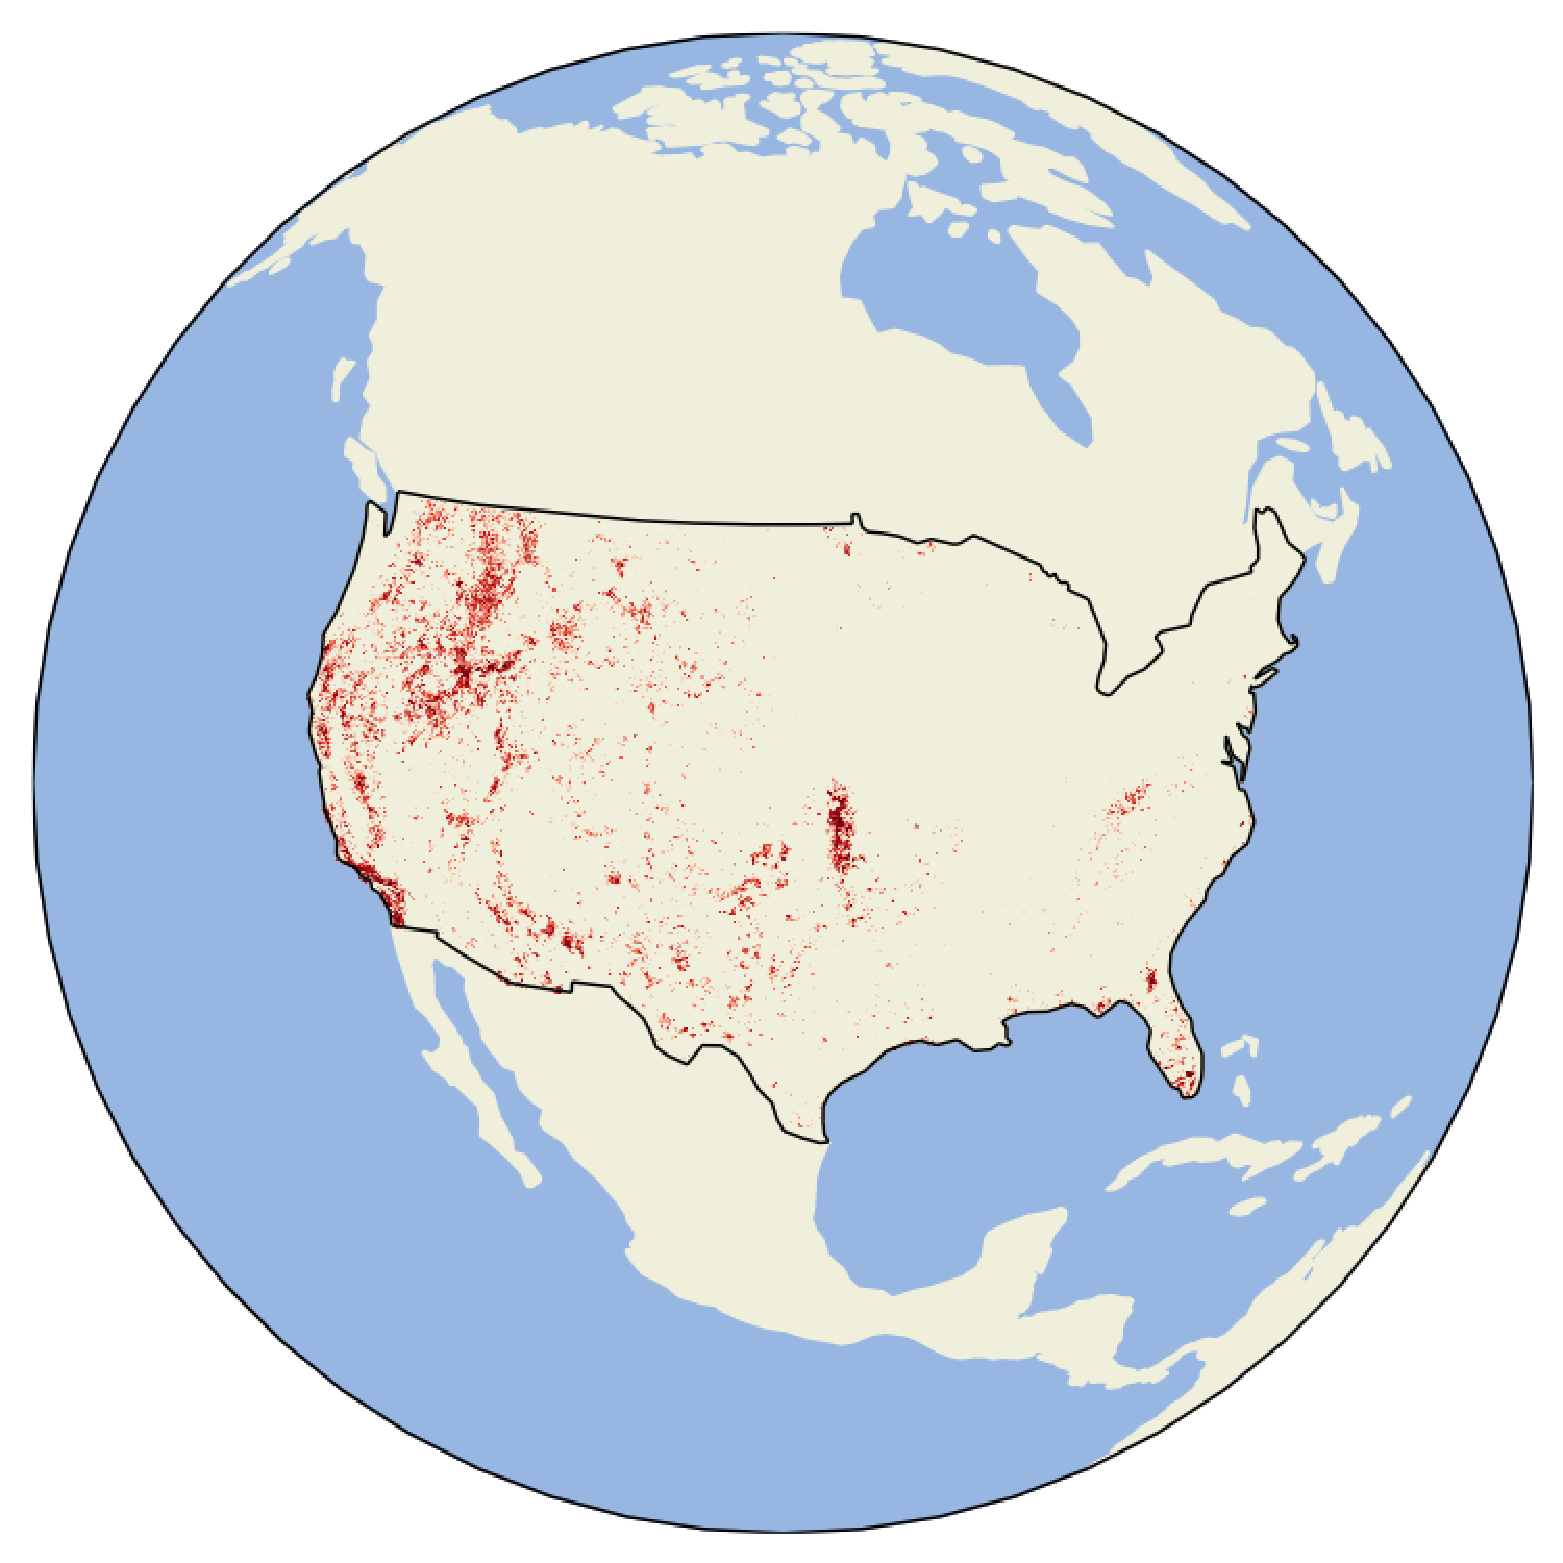
\includegraphics[width=0.5\linewidth]{images/constraind_diffusion_rejection/wildfire_data_dist.pdf}
	\caption{Orthographic projection of the wildfire dataset described in~\Cref{app_sec:wildfire_data}.
		The projection is aligned with the centroid of the continental United States and zoomed in ten-fold for visual clarity.
		All visualisations of geospatial data were generated using the \textsc{GeoViews} \parencite{geoviews} and \textsc{DataShader} \cite{datashader} libraries.
	}
	\label{fig_app:wildfire_data_subsample}
\end{figure}

\subsection{Point-in-spherical-polytope algorithms}
\label{app_sec:wildfire_data_algo}

The support of the data-generating distribution we aim to approximate is thus restricted to a highly non-convex spherical polytope $\mathbb{P}\in\c{S}^2$ given by the country borders of the continental United States.
To determine whether a query point $q\in\c{S}^2$ is within $\mathbb{P}$, we adapt an efficient reformulation of the point-in-spherical-polygon algorithm \parencite{bevis1989locating} presented in \cite{ketzner2022robust}.
The algorithm requires the provision of a reference point $r\in\c{S}^2$ known to be located in $\mathbb{P}$ and determines whether $q$ is inside or outside the polygon by checking whether the geodesic between $r$ and $q$ crosses the polygon an even or odd number of times.
Letting $\Hat{x}\in\mathbb{R}^3$ denote the Cartesian coordinates of a point $x\in\c{S}^2$, \cite{ketzner2022robust} rely on a Cartesian reference coordinate system $\Hat{Q}$ (with its $z$-axis given by $\Hat{r}$) and the corresponding spherical coordinate system $Q$ to decompose the edge-crossing condition of \textcite{bevis1989locating} into two efficiently computable parts.
That is, the geodesic between $q$ and $r$ crosses an edge $e_i=(v_i, v_j)$ of the polygon if: \begin{enumerate}[label=(\roman*)] \item the longitude of $q$ in $Q$ is bounded by the longitudes of $v_i$ and $v_j$ in $Q$, i.e. $$ \phi_{Q}(q)\in[\min(\phi_{Q}(v_i), \phi_{Q}(v_j)), \max(\phi_{Q}(v_i), \phi_{Q}(v_j))], $$ \item the plane specified by the normal vector $\Hat{p}_i=\Hat{v}_i\times \Hat{v}_j$ represents an equator that separates ${q}$ and ${r}$ into two different hemispheres, i.e. $$ \operatorname{sign}(\langle \Hat{p}_i, \Hat{r} \rangle \cdot \langle \Hat{p}_i, \Hat{q} \rangle) = -1.
	      $$
\end{enumerate}

Especially when $\mathbb{P}$ is fixed and the corresponding coordinate transformations and normal vectors can be precomputed for each edge, this algorithm affords an efficient and parallelisable approach to determining whether any given point on $\c{S}^2$ is contained by a spherical polytope.

\section{Supplementary Experimental Results}
\label{sec:experimental_appendix}

\subsection{Evaluating log-barrier models}
\label{sec:app_exp_barrier_results}

Following \cite{fishman2023diffusion}, we approached the empirical evaluation of our Metropolis model by computing the maximum mean discrepancy (MMD) \parencite{gretton2012kernel} between samples from the true distribution and the trained diffusion models.
The MMD is a statistic that quantifies the similarity of two samples by computing the distance of their respective mean embeddings in a reproducing kernel Hilbert space.
For this, we use an RBF kernel with the same length scales as the standard deviations of the normal distributions used to generate the synthetic distribution.
We sum these RBF kernels by the weights of the corresponding components of the synthetic Gaussian mixture model.

\begin{table}[H]
	\caption{
		Maximum mean discrepancy (MMD) ($\downarrow$) of a held-out test set from a synthetic bimodal distribution over convex subsets of $\R^d$ bounded by the hypercube \([-1,1]^d\) and unit simplex \(\Delta^d\).
		Means and standard deviations are computed over 3 different runs.
	}
	\label{tab:synthetic_polytope_mmd}
	\vspace{1em}
	\centering

	\begin{tabular}{cllll}
		\toprule
		Constraint & \(d\) & {Log-Barrier}      & {Reflected}        & {Metropolis}                \\
		\midrule
		\multirow{3}{*}{$[-1,1]^d$}
		           & 2     & $0.066 \pm{0.006}$ & $0.055 \pm{0.015}$ & $\mathbf{0.029 \pm{0.002}}$ \\
		           & 3     & $0.209 \pm{0.077}$ & $0.080 \pm{0.004}$ & $\mathbf{0.047 \pm{0.006}}$ \\
		           & 10    & $0.330 \pm{0.004}$ & $0.313 \pm{0.048}$ & $\mathbf{0.226 \pm{0.006}}$ \\
		\midrule
		\multirow{3}{*}{$\Delta^d$}
		           & 2     & $0.050 \pm{0.012}$ & $0.043 \pm{0.002}$ & $\mathbf{0.032 \pm{0.007}}$ \\
		           & 3     & $0.238 \pm{0.009}$ & $0.181 \pm{0.007}$ & $\mathbf{0.121 \pm{0.010}}$ \\
		           & 10    & $0.275 \pm{0.015}$ & $0.290 \pm{0.009}$ & $\mathbf{0.267 \pm{0.003}}$ \\
		\bottomrule
	\end{tabular}
\end{table}

From the results in~\Cref{tab:synthetic_polytope_mmd}, it is clear that the log-barrier approach performs significantly worse than the Reflected model across all but one and worse than the Metropolis models across all settings.
This, in conjunction with numerical instabilities we encountered when attempting to evaluate sample likelihoods with the log-barrier models as presented in \cite{fishman2023diffusion}, motivated us to focus on the Reflected and Metropolis models in the main text.

\subsection{Implementational details}
\label{sec:app_implementational_details}

An anonymised repository with the datasets and code necessary to reproduce our experiments can be found under the following links: The main repository is available \href{https://anonymous.4open.science/r/constrained-diffusion-models/}{here} and the supporting package which handles the geometry can be found under \href{https://anonymous.4open.science/r/geomstats-with-boundary/}{here}.

We use the same architecture in all of our experiments: a 6-layer MLP with 512 hidden units and sine activation functions, except in the output layer, which uses a linear activation function.
Following \cite{fishman2023diffusion}, we implement a simple linear function that scales the score by the distance to the boundary, approaching zero within $\epsilon = 0.01$ of the boundary.
This ensures the score obeys the Neumann boundary conditions required by the reflected Brownian Motion.
For the geospatial dataset within non-convex country borders, we do not use distance rescaling.
Instead, we substitute it with a series of step functions to rescale the score.
This is a proof-of-concept to show that even when computing the distance is hard, simple and efficient approximations suffice.
When constructing Riemannian diffusion models on the torus and sphere for the protein and geospatial datasets, we follow \cite{debortoli2022riemannian} and include an additional preconditioner for the score on the manifold.
We \emph{do not} use the residual trick or the standard deviation trick, which are both common score-rescaling functions in image model architectures; in our setting, we find that they adversely affect model training.

For the forward/reverse process we always set $T=1$, $\beta_0=\num{1e-3}$ and then tune $\beta_1$ to ensure that the forward process just reaches the invariant distribution with a linear $\beta$-schedule.
At sampling time we use $N=100$ steps of the discretised process.
We discretise the training process by selecting a random $N$ between 0 and 100 for each example, rolling out to that time point.
This lets us cheaply implement a simple variance reduction technique: we take multiple samples from this trajectory by selecting multiple random $N$ to save for each example.
This technique was originally described in \cite{fishman2023diffusion} and we find it is also helpful for our Metropolis models.
For all experiments, we use the $\mathrm{ism}$ loss with a modified weighting function of $(1 + t)$, which we found to be essential to model training.
All experiments use a batch size of 256 with 8 repeats per batch.
For training, we use a learning rate of \num{2e-4} with a cosine learning rate schedule.
We trained for 100,000 batches on the synthetic examples and 300,000 batches on the real-world examples (robotics, proteins, wildfires).

We selected these hyperparameters from a systematic search over learning rates (\num{6e-4}, \num{2e-4}, \num{6e-5}, \num{2e-5}), learning rate schedules (cosine, log-linear), and batch sizes (128, 256, 512, 1024) on synthetic examples for the reflected and log-barrier models.
Similar parameters worked well for both, and we used those for our Metropolis models to allow a straightforward comparison.
We tried $N=100,1000$ for several synthetic examples but found that very large rollout times actually hurt performance for the Metropolis model, though the log-barrier performed a bit better with longer rollouts and the reflected was the same.

All models were trained on a single NVIDIA GeForce GTX 1080 GPU.
All of the Metropolis models presented here can easily be trained on this hardware in under 4 hours.
The runtime for the log-barrier and reflected models is considerably longer.

\subsection{Synthetic Distributions on Constrained Manifolds of Increasing Dimensionality}
\label{sec:app_exp_synthetic_tasks}

\begin{figure}[H]
	\centering
	\begin{subfigure}{.23\textwidth}
		\centering
		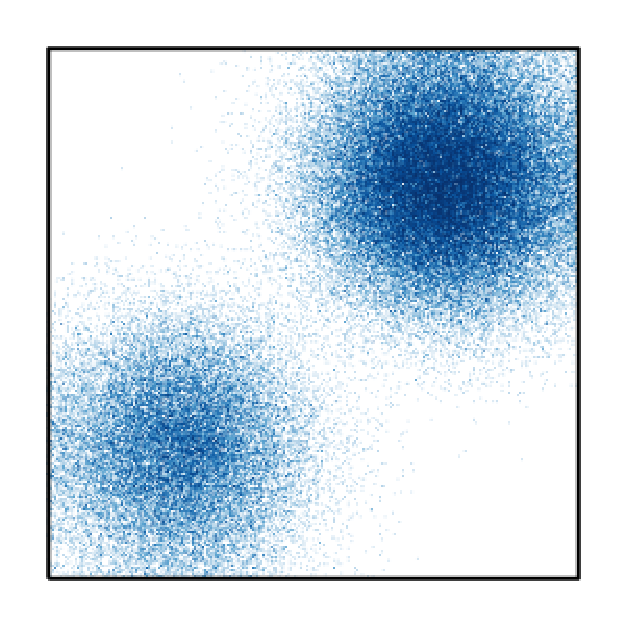
\includegraphics[width=\textwidth]{images/constraind_diffusion_rejection/synthetic_data/synthetic_hypercube_2d_data.pdf}
		\caption{Data distribution}
		\label{fig:app:synthetic_hypercube_data}
	\end{subfigure}
	\begin{subfigure}{.23\textwidth}
		\centering
		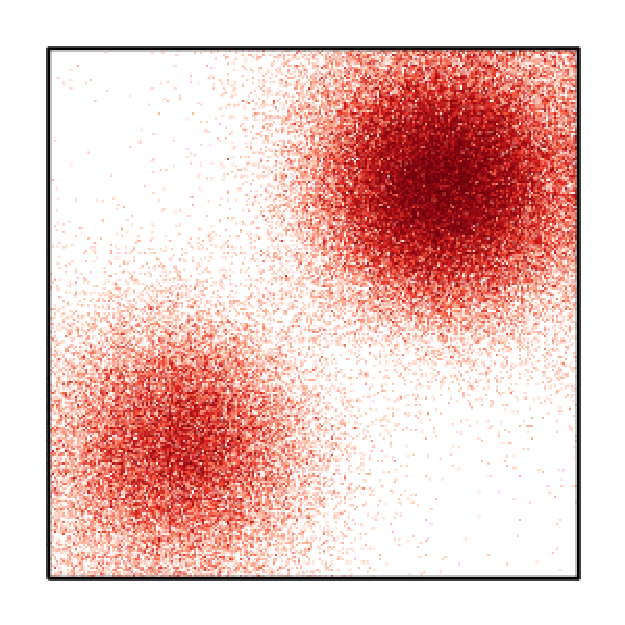
\includegraphics[width=\textwidth]{images/constraind_diffusion_rejection/synthetic_data/synthetic_hypercube_2d_rejection.pdf}
		\caption{Metropolis model}
		\label{fig:app:synthetic_hypercube_rejection}
	\end{subfigure}
	\begin{subfigure}{.23\textwidth}
		\centering
		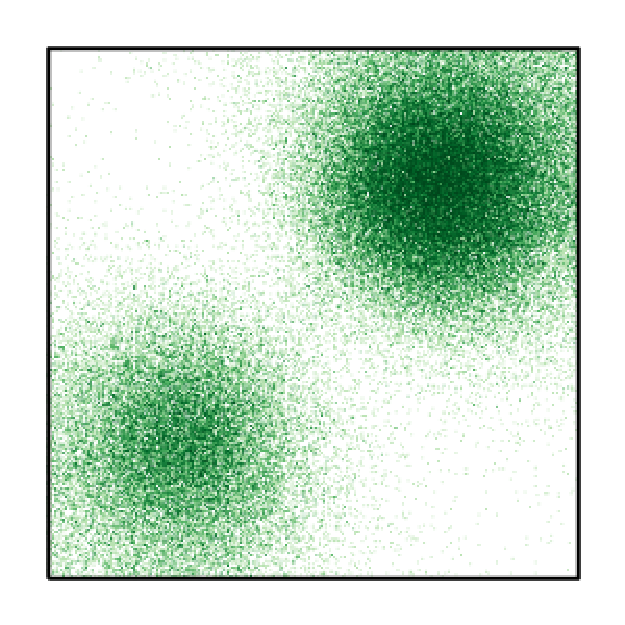
\includegraphics[width=\textwidth]{images/constraind_diffusion_rejection/synthetic_data/synthetic_hypercube_2d_reflected.pdf}
		\caption{Reflected model}
		\label{fig:app:synthetic_hypercube_reflected}
	\end{subfigure}
	\begin{subfigure}{.23\textwidth}
		\centering
		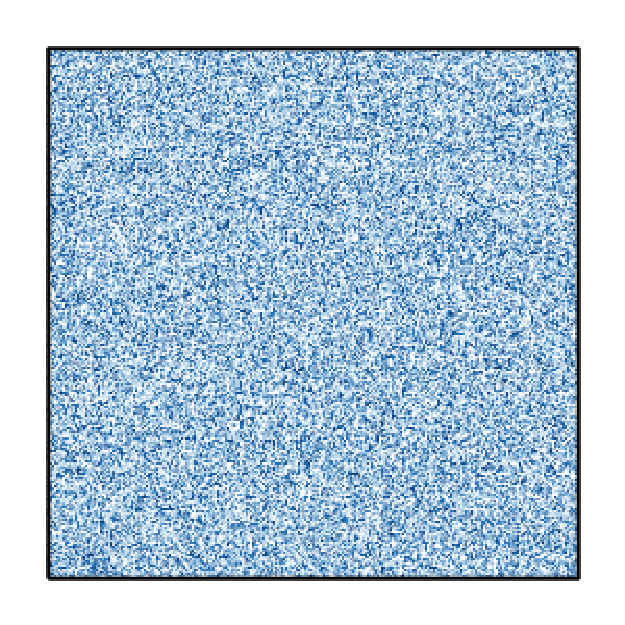
\includegraphics[width=\textwidth]{images/constraind_diffusion_rejection/synthetic_data/synthetic_hypercube_2d_uniform.pdf}
		\caption{Uniform distribution}
		\label{fig:app:synthetic_hypercube_uniform}
	\end{subfigure}
	\caption{Qualitiative comparison of samples from the data distribution, our Metropolis model, a Reflected model and the uniform distribution for a synthetic bimodal distribution on $[-1, 1]^2$.}
	\label{fig:app:synthetic_hypercube}
\end{figure}

\begin{figure}[H]
	\centering
	\begin{subfigure}{.23\textwidth}
		\centering
		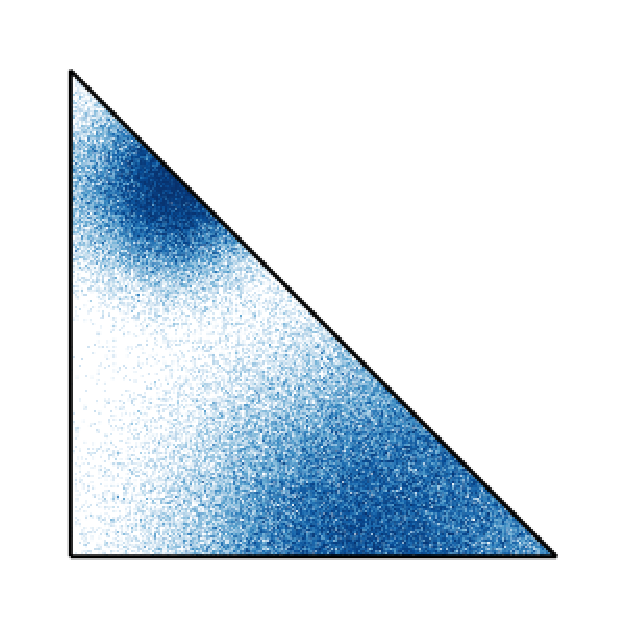
\includegraphics[width=\textwidth]{images/constraind_diffusion_rejection/synthetic_data/synthetic_dirichlet_2d_data.pdf}
		\caption{Data distribution}
		\label{fig:app:synthetic_simplex_data}
	\end{subfigure}
	\begin{subfigure}{.23\textwidth}
		\centering
		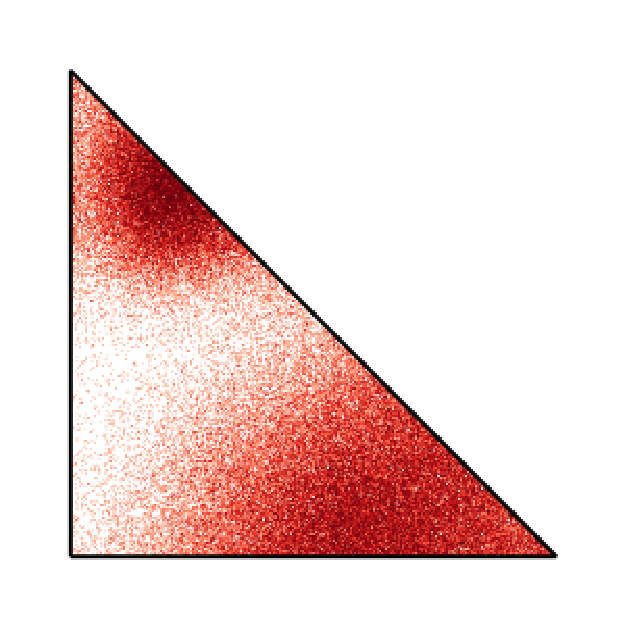
\includegraphics[width=\textwidth]{images/constraind_diffusion_rejection/synthetic_data/synthetic_dirichlet_2d_rejection.pdf}
		\caption{Metropolis model}
		\label{fig:app:synthetic_simplex_rejection}
	\end{subfigure}
	\begin{subfigure}{.23\textwidth}
		\centering
		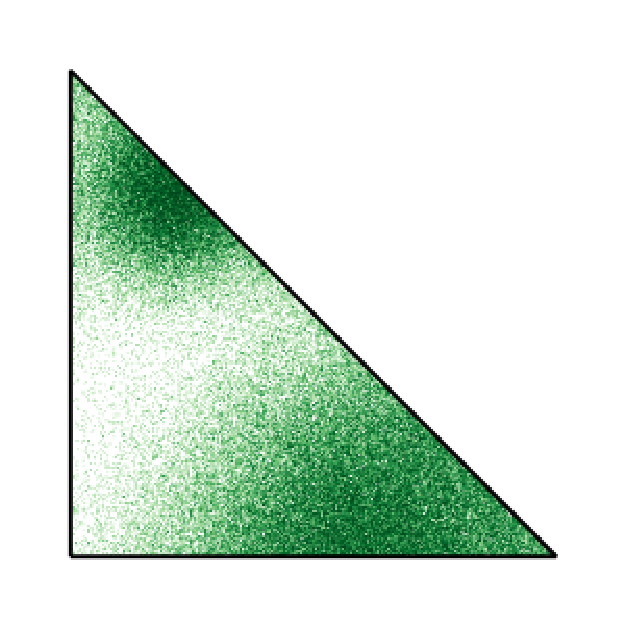
\includegraphics[width=\textwidth]{images/constraind_diffusion_rejection/synthetic_data/synthetic_dirichlet_2d_reflected.pdf}
		\caption{Reflected model}
		\label{fig:app:synthetic_simplex_reflected}
	\end{subfigure}
	\begin{subfigure}{.23\textwidth}
		\centering
		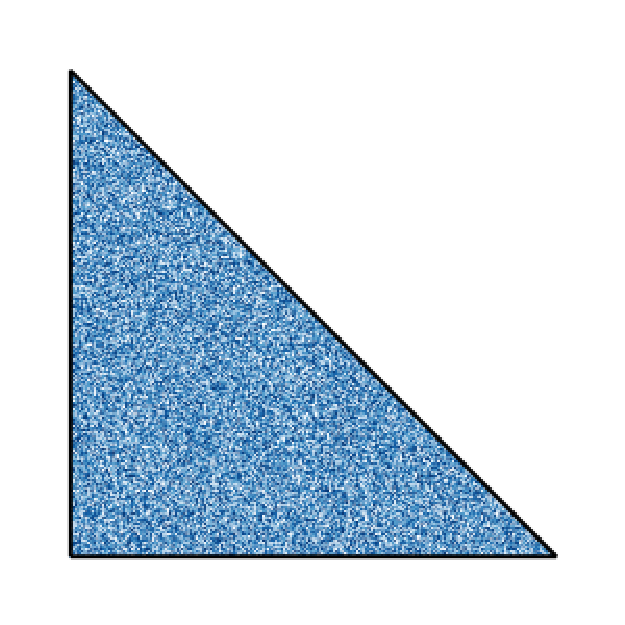
\includegraphics[width=\textwidth]{images/constraind_diffusion_rejection/synthetic_data/synthetic_dirichlet_2d_uniform.pdf}
		\caption{Uniform distribution}
		\label{fig:app:synthetic_simplex_uniform}
	\end{subfigure}
	\caption{Qualitiative comparison of samples from the data distribution, our Metropolis model, a Reflected model and the uniform distribution for a synthetic bimodal distribution on $\Delta^2$.}
	\label{fig:app:synthetic_simplex}
\end{figure}

\subsection{Constrained Configurational Modelling of Robotic Arms}
\label{sec:app_robotic_arms_spd}

The following univariate marginal and pairwise bivariate plots visualise the distribution of different samples in \begin{enumerate}[label=(\roman*)] \item the three dimensions needed to describe an ellipsoid \(M=\begin{bmatrix} l_{1} & l_{2}\\ l_{2} & l_3 \end{bmatrix}\in\c{S}_{++}^2\) and \item the two dimensions needed to describe a location in \(\R^2\).
\end{enumerate}

\subsubsection{Visualisation of samples from the data distribution}

\begin{figure}[H]
	\centering
	\begin{subfigure}[t]{0.45\textwidth}
		\centering
		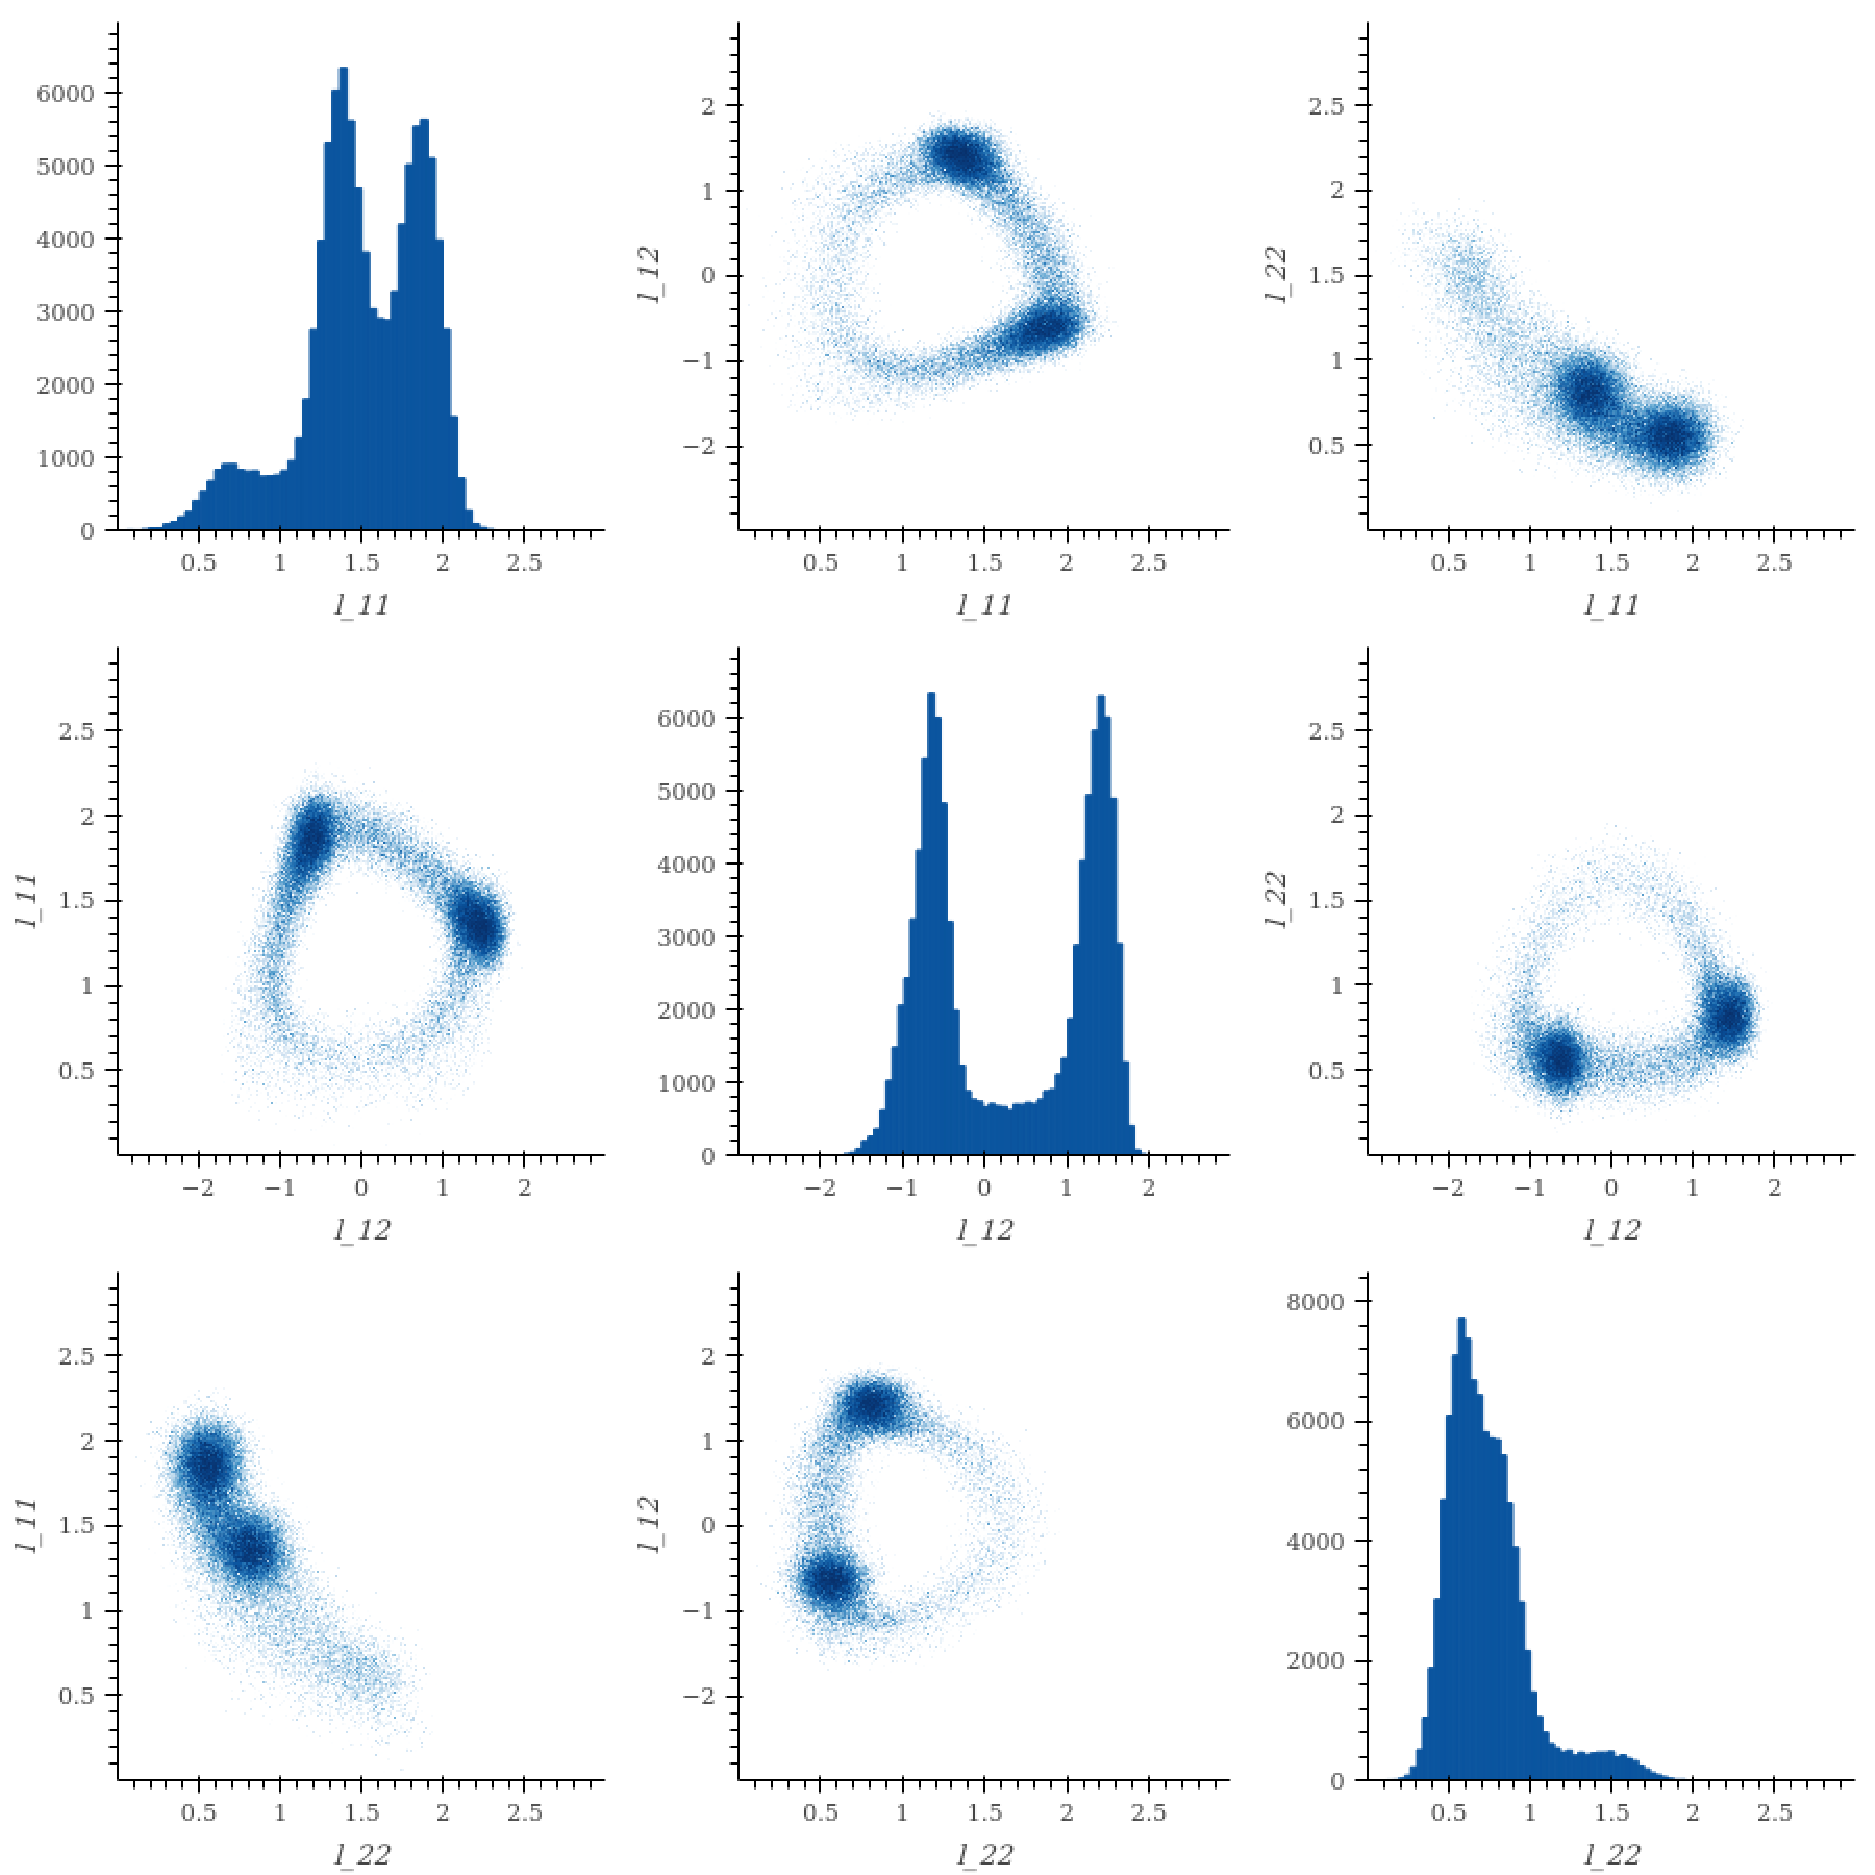
\includegraphics[width=\textwidth]{images/constraind_diffusion_rejection/pairplots/spd_data_ll.pdf}
		\caption{Plots of the univariate marginal and pairwise bivariate distributions of \num{1e5} samples from the data distribution in \(\c{S}_{++}^2\).}
		\label{fig:app_pairplots_robot_data_ellips}
	\end{subfigure}
	\hfill
	\begin{subfigure}[t]{0.45\textwidth}
		\centering
		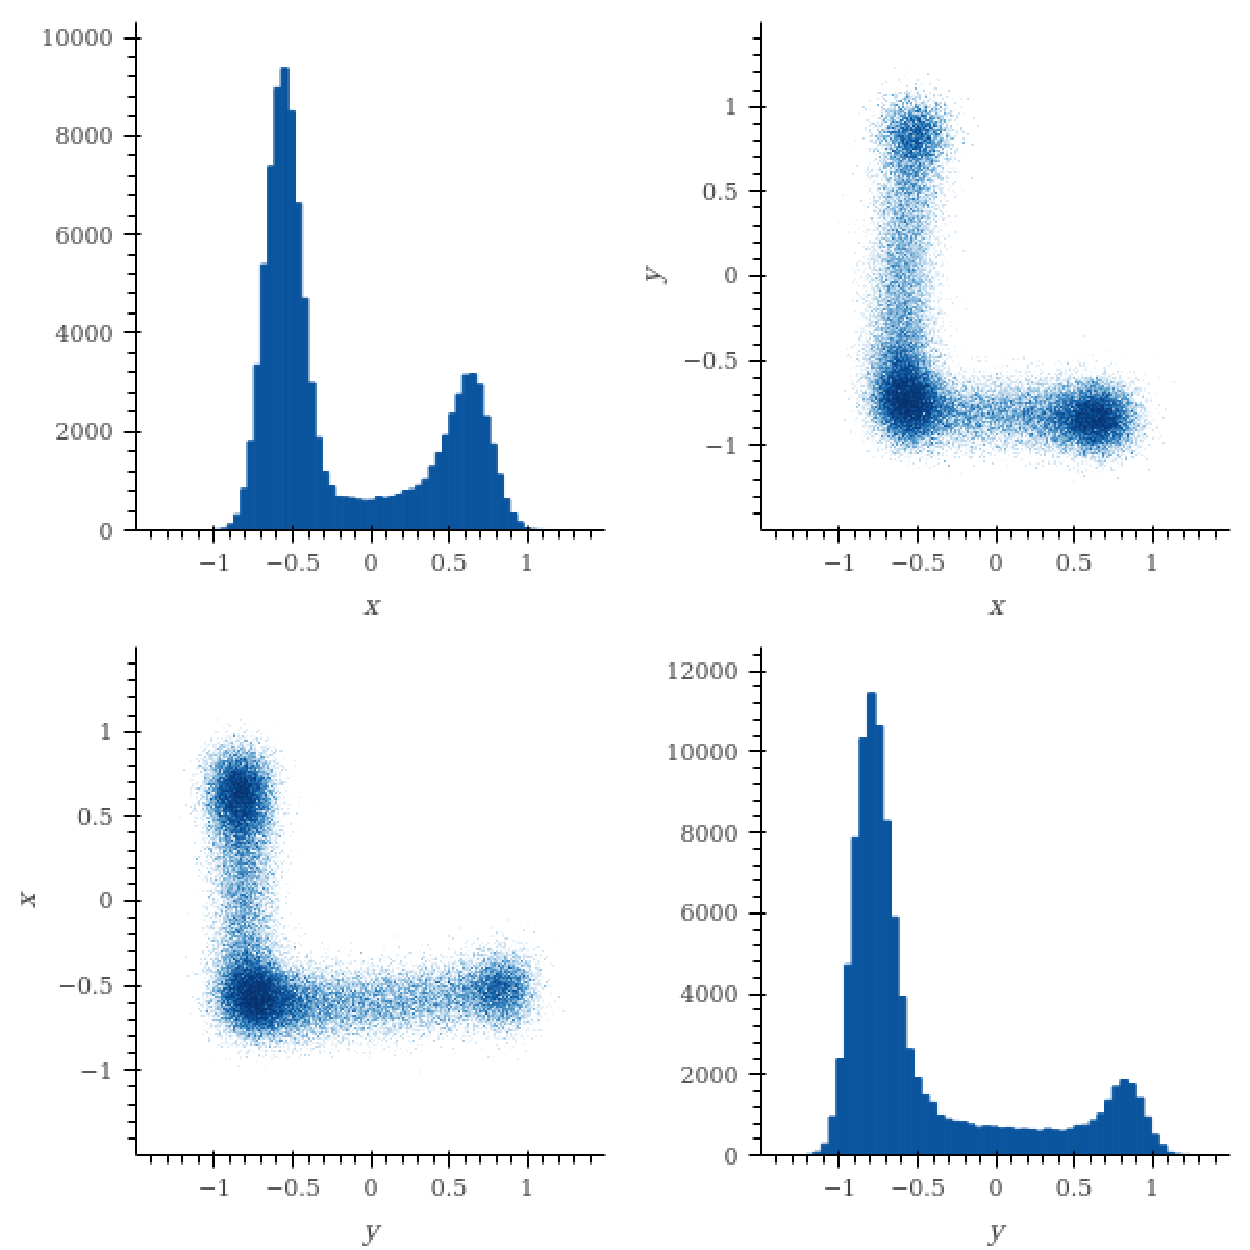
\includegraphics[width=\textwidth]{images/constraind_diffusion_rejection/pairplots/spd_data_xy.pdf}
		\caption{Plots of the univariate marginal and pairwise bivariate distributions of \num{1e5} samples from the data distribution in \(\R^2\).}
		\label{fig:app_pairplots_robot_data_location}
	\end{subfigure}
	\caption{Visualisation of the data distribution in \(\c{S}_{++}^2\times\R^2\) using univariate marginal and pairwise bivariate plots.}
	\label{fig:app_pairplots_robot_data}
\end{figure}

\subsubsection{Visualisation of samples from our Metropolis sampling-based diffusion model}

\begin{figure}[H]
	\centering
	\begin{subfigure}[t]{0.45\textwidth}
		\centering
		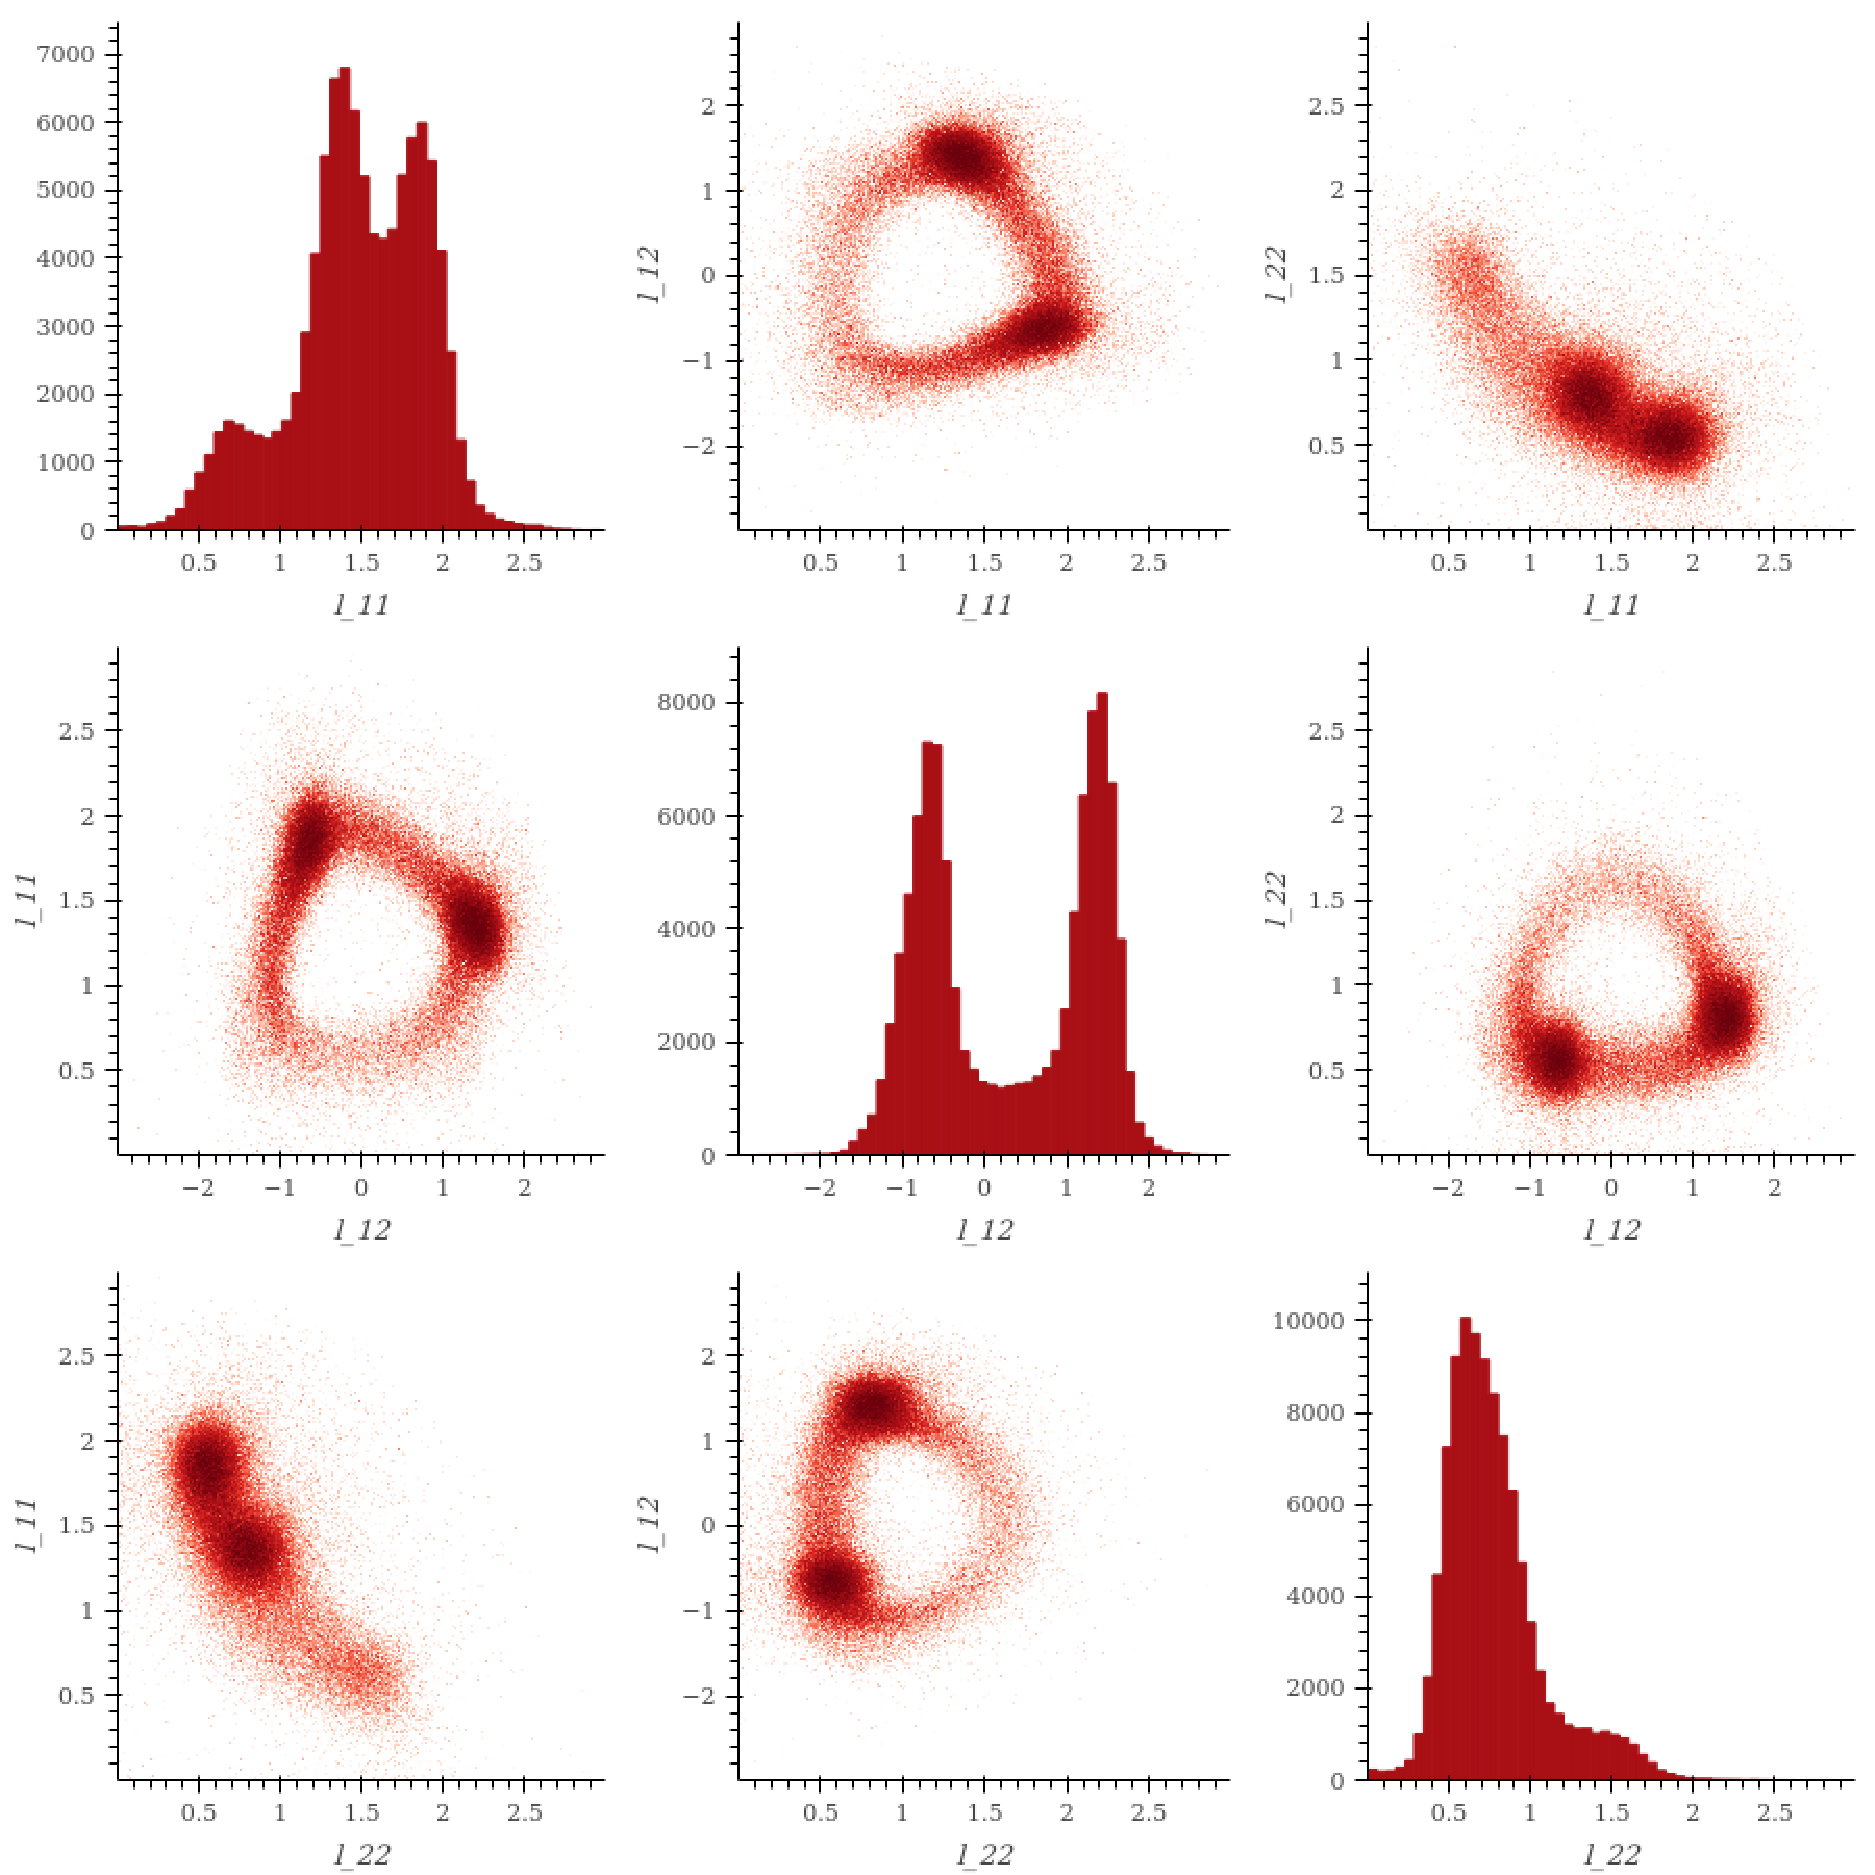
\includegraphics[width=\textwidth]{images/constraind_diffusion_rejection/pairplots/spd_rejection_ll.pdf}
		\caption{Plots of the univariate marginal and pairwise bivariate distributions of \num{1e5} samples from our Metropolis sampling-based diffusion model in \(\c{S}_{++}^2\).}
		\label{fig:app_pairplots_robot_rejection_ellips}
	\end{subfigure}
	\hfill
	\begin{subfigure}[t]{0.45\textwidth}
		\centering
		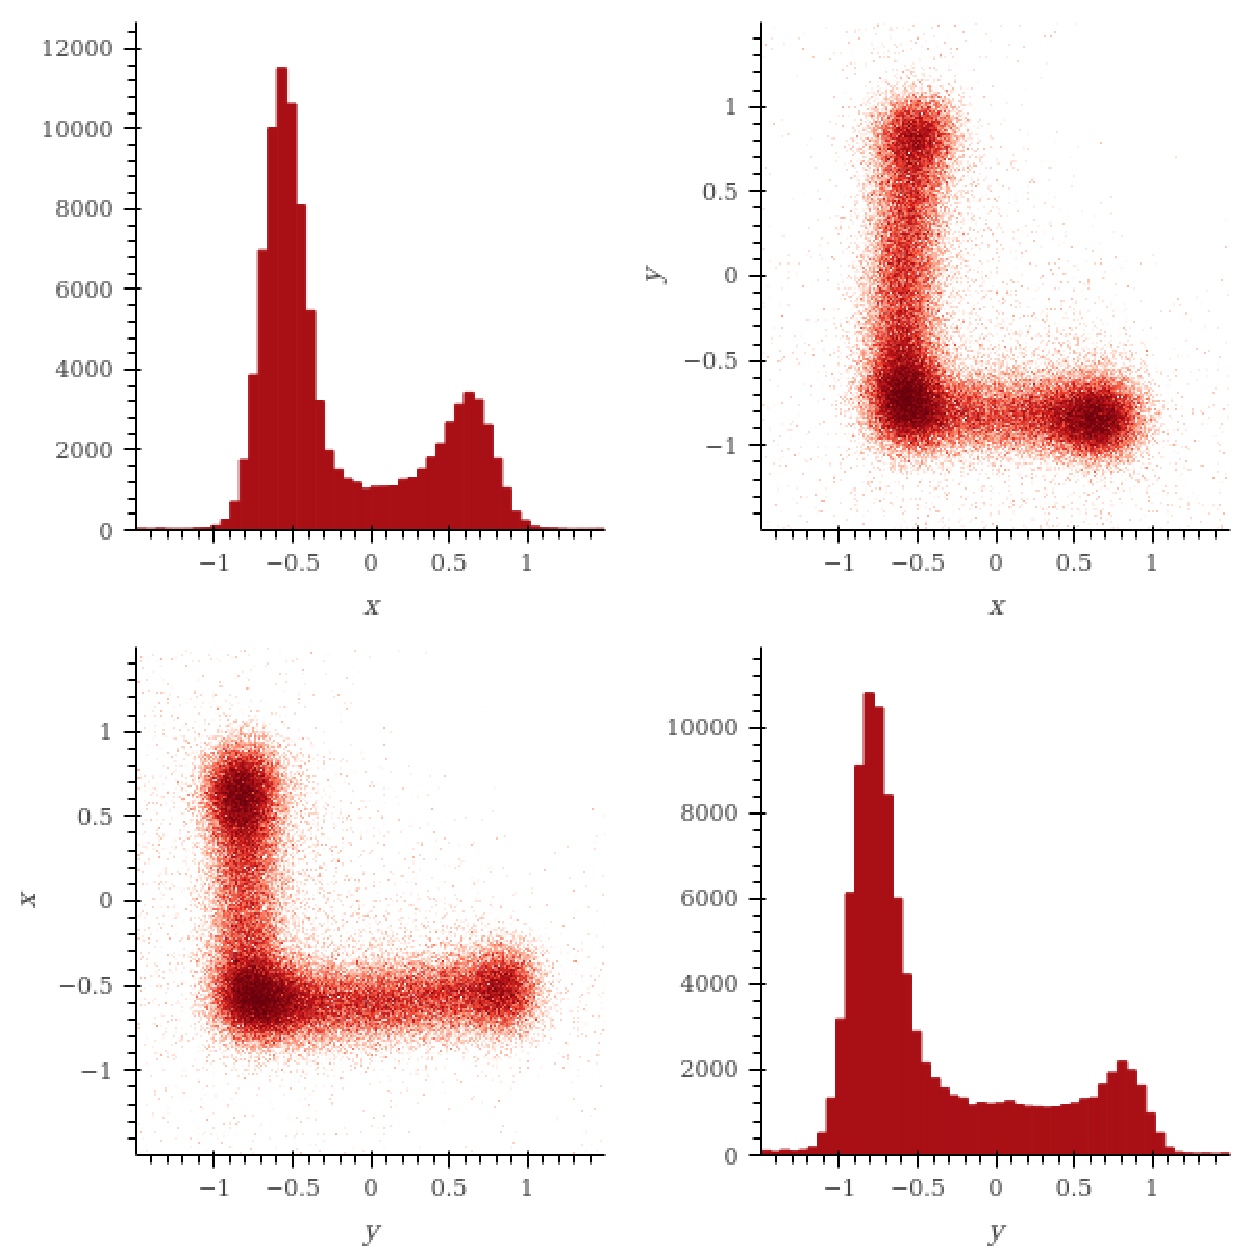
\includegraphics[width=\textwidth]{images/constraind_diffusion_rejection/pairplots/spd_rejection_xy.pdf}
		\caption{Plots of the univariate marginal and pairwise bivariate distributions of \num{1e5} samples from our Metropolis sampling-based diffusion model in \(\R^2\).}
		\label{fig:app_pairplots_robot_rejection_location}
	\end{subfigure}
	\caption{Visualisation of the distribution learned by our Metropolis sampling-based diffusion model in \(\c{S}_{++}^2\times\R^2\) using univariate marginal and pairwise bivariate plots.}
	\label{fig:app_pairplots_robot_rejection}
\end{figure}

\subsubsection{Visualisation of samples from a reflected Brownian motion-based diffusion model}

\begin{figure}[H]
	\centering
	\begin{subfigure}[t]{0.45\textwidth}
		\centering
		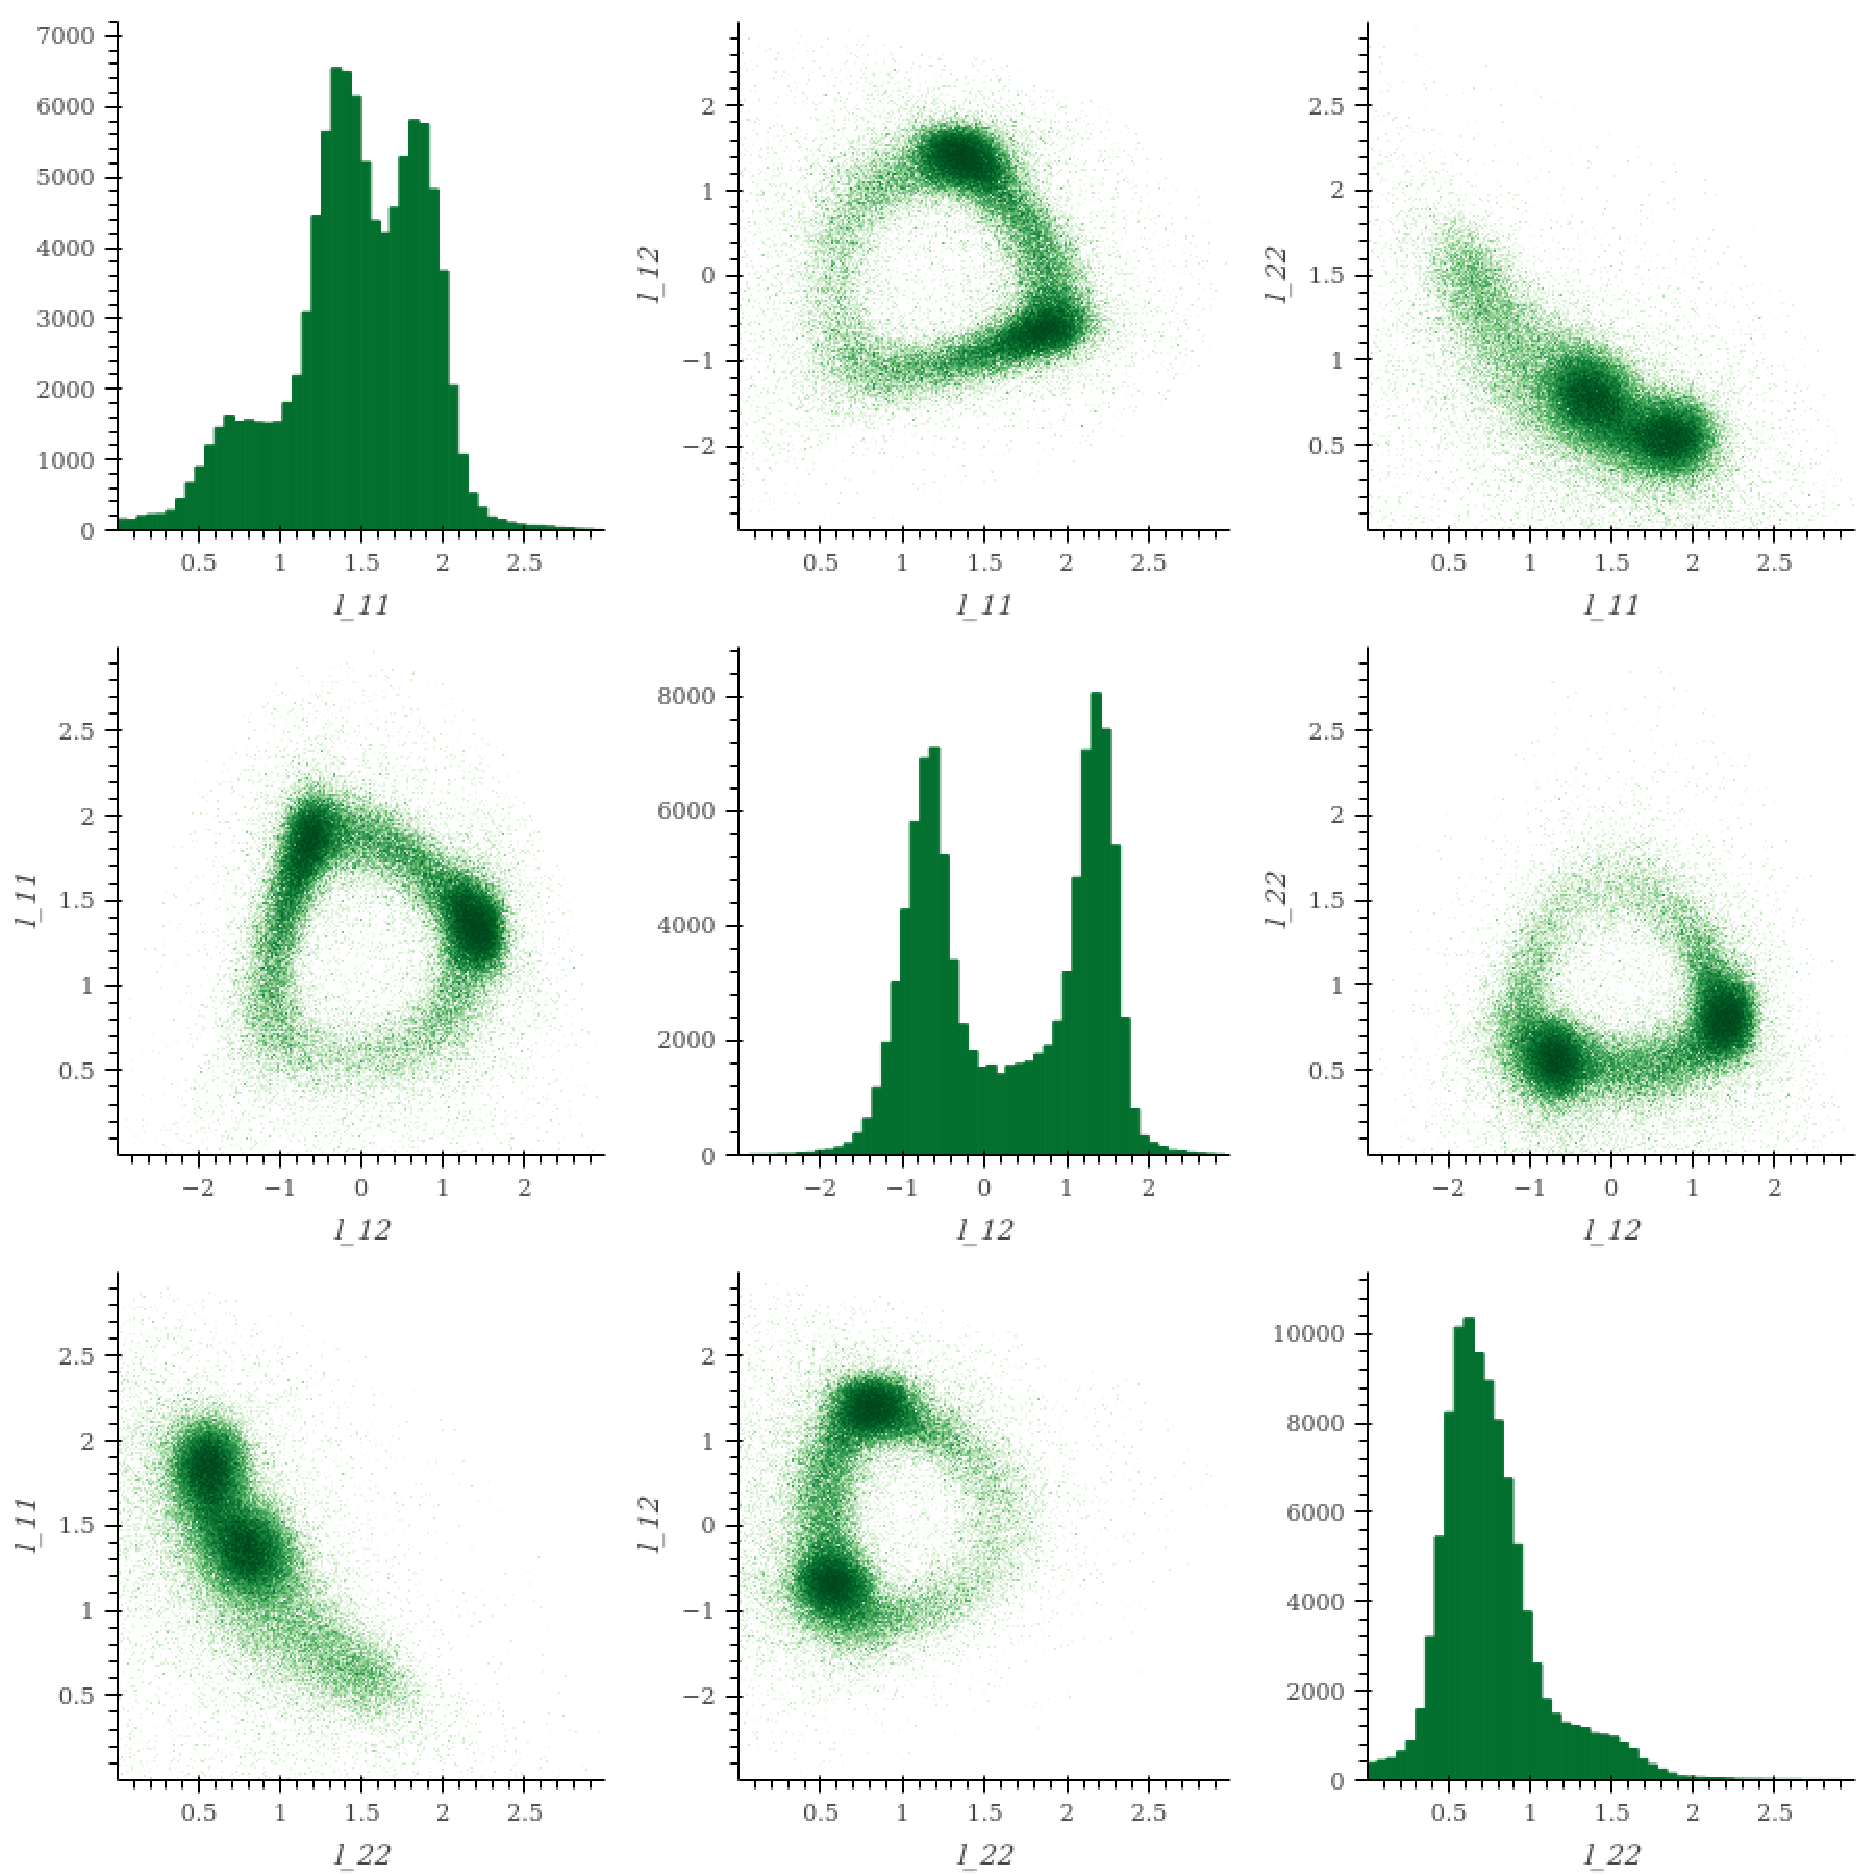
\includegraphics[width=\textwidth]{images/constraind_diffusion_rejection/pairplots/spd_reflection_ll.pdf}
		\caption{Plots of the univariate marginal and pairwise bivariate distributions of \num{1e5} samples from a reflected Brownian motion-based diffusion model in \(\c{S}_{++}^2\).}
		\label{fig:app_pairplots_robot_reflected_ellips_dupref}
	\end{subfigure}
	\hfill
	\begin{subfigure}[t]{0.45\textwidth}
		\centering
		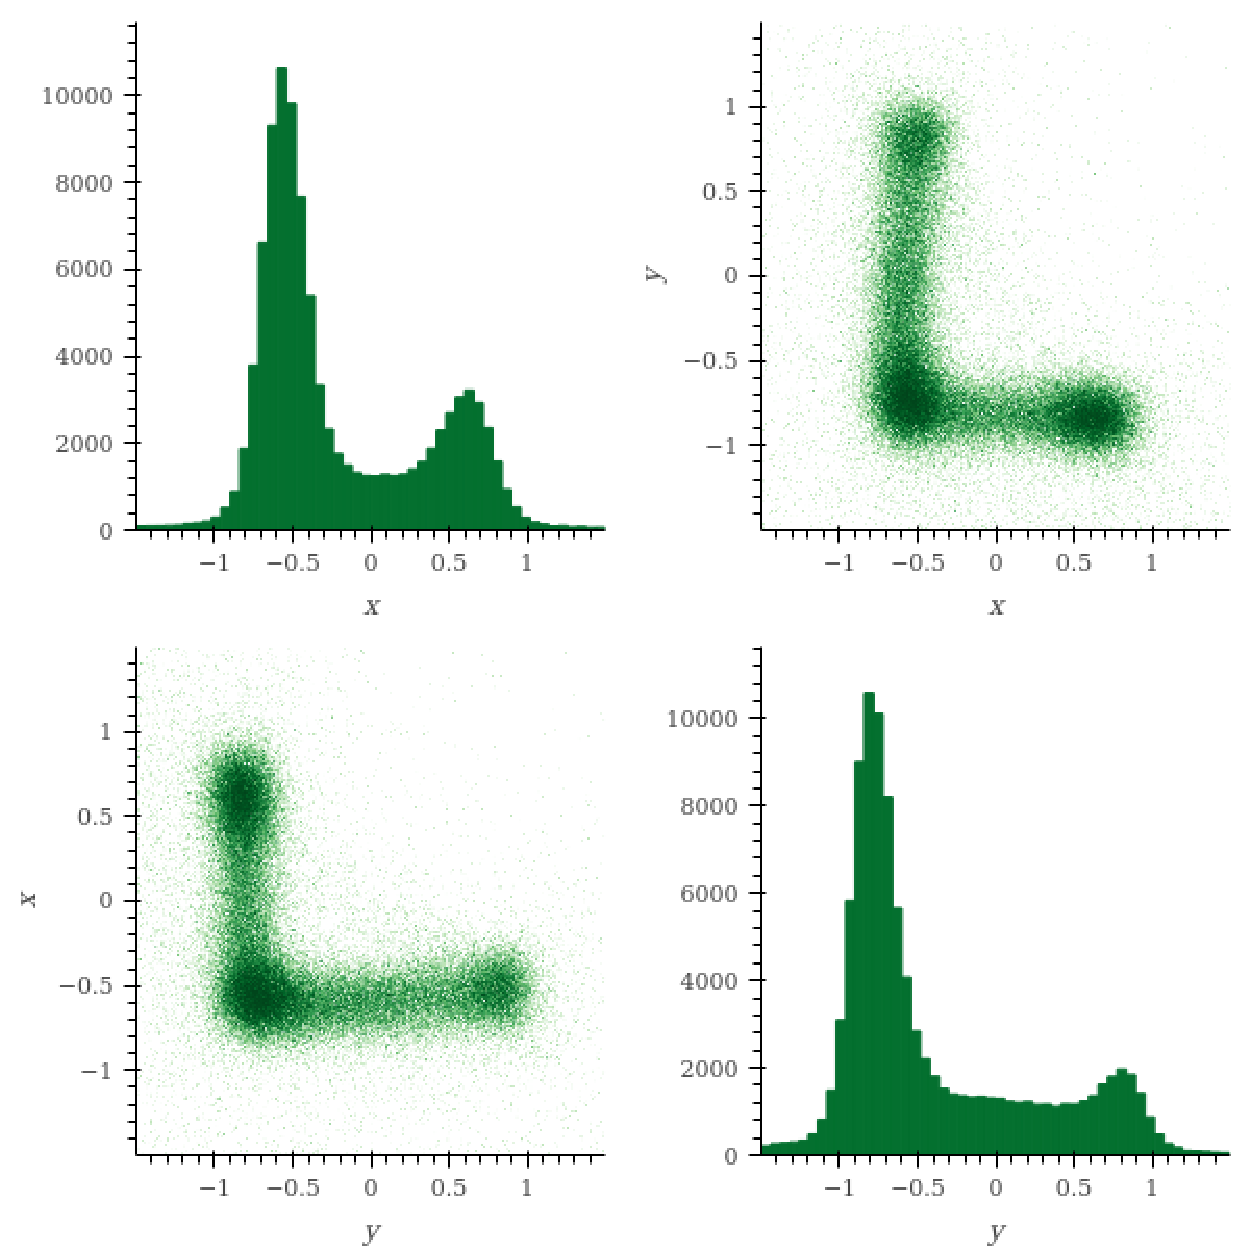
\includegraphics[width=\textwidth]{images/constraind_diffusion_rejection/pairplots/spd_reflection_xy.pdf}
		\caption{Plots of the univariate marginal and pairwise bivariate distributions of \num{1e5} samples from a reflected Brownian motion-based diffusion model in \(\R^2\).}
		\label{fig:app_pairplots_robot_reflected_location_dupref}
	\end{subfigure}
	\caption{Visualisation of the distribution learned by a reflected Brownian motion-based diffusion model in \(\c{S}_{++}^2\times\R^2\) using univariate marginal and pairwise bivariate plots.}
	\label{fig:app_pairplots_robot_reflected_dupref}
\end{figure}

\subsubsection{Visualisation of samples from the uniform distribution}

\begin{figure}[H]
	\centering
	\begin{subfigure}[t]{0.45\textwidth}
		\centering
		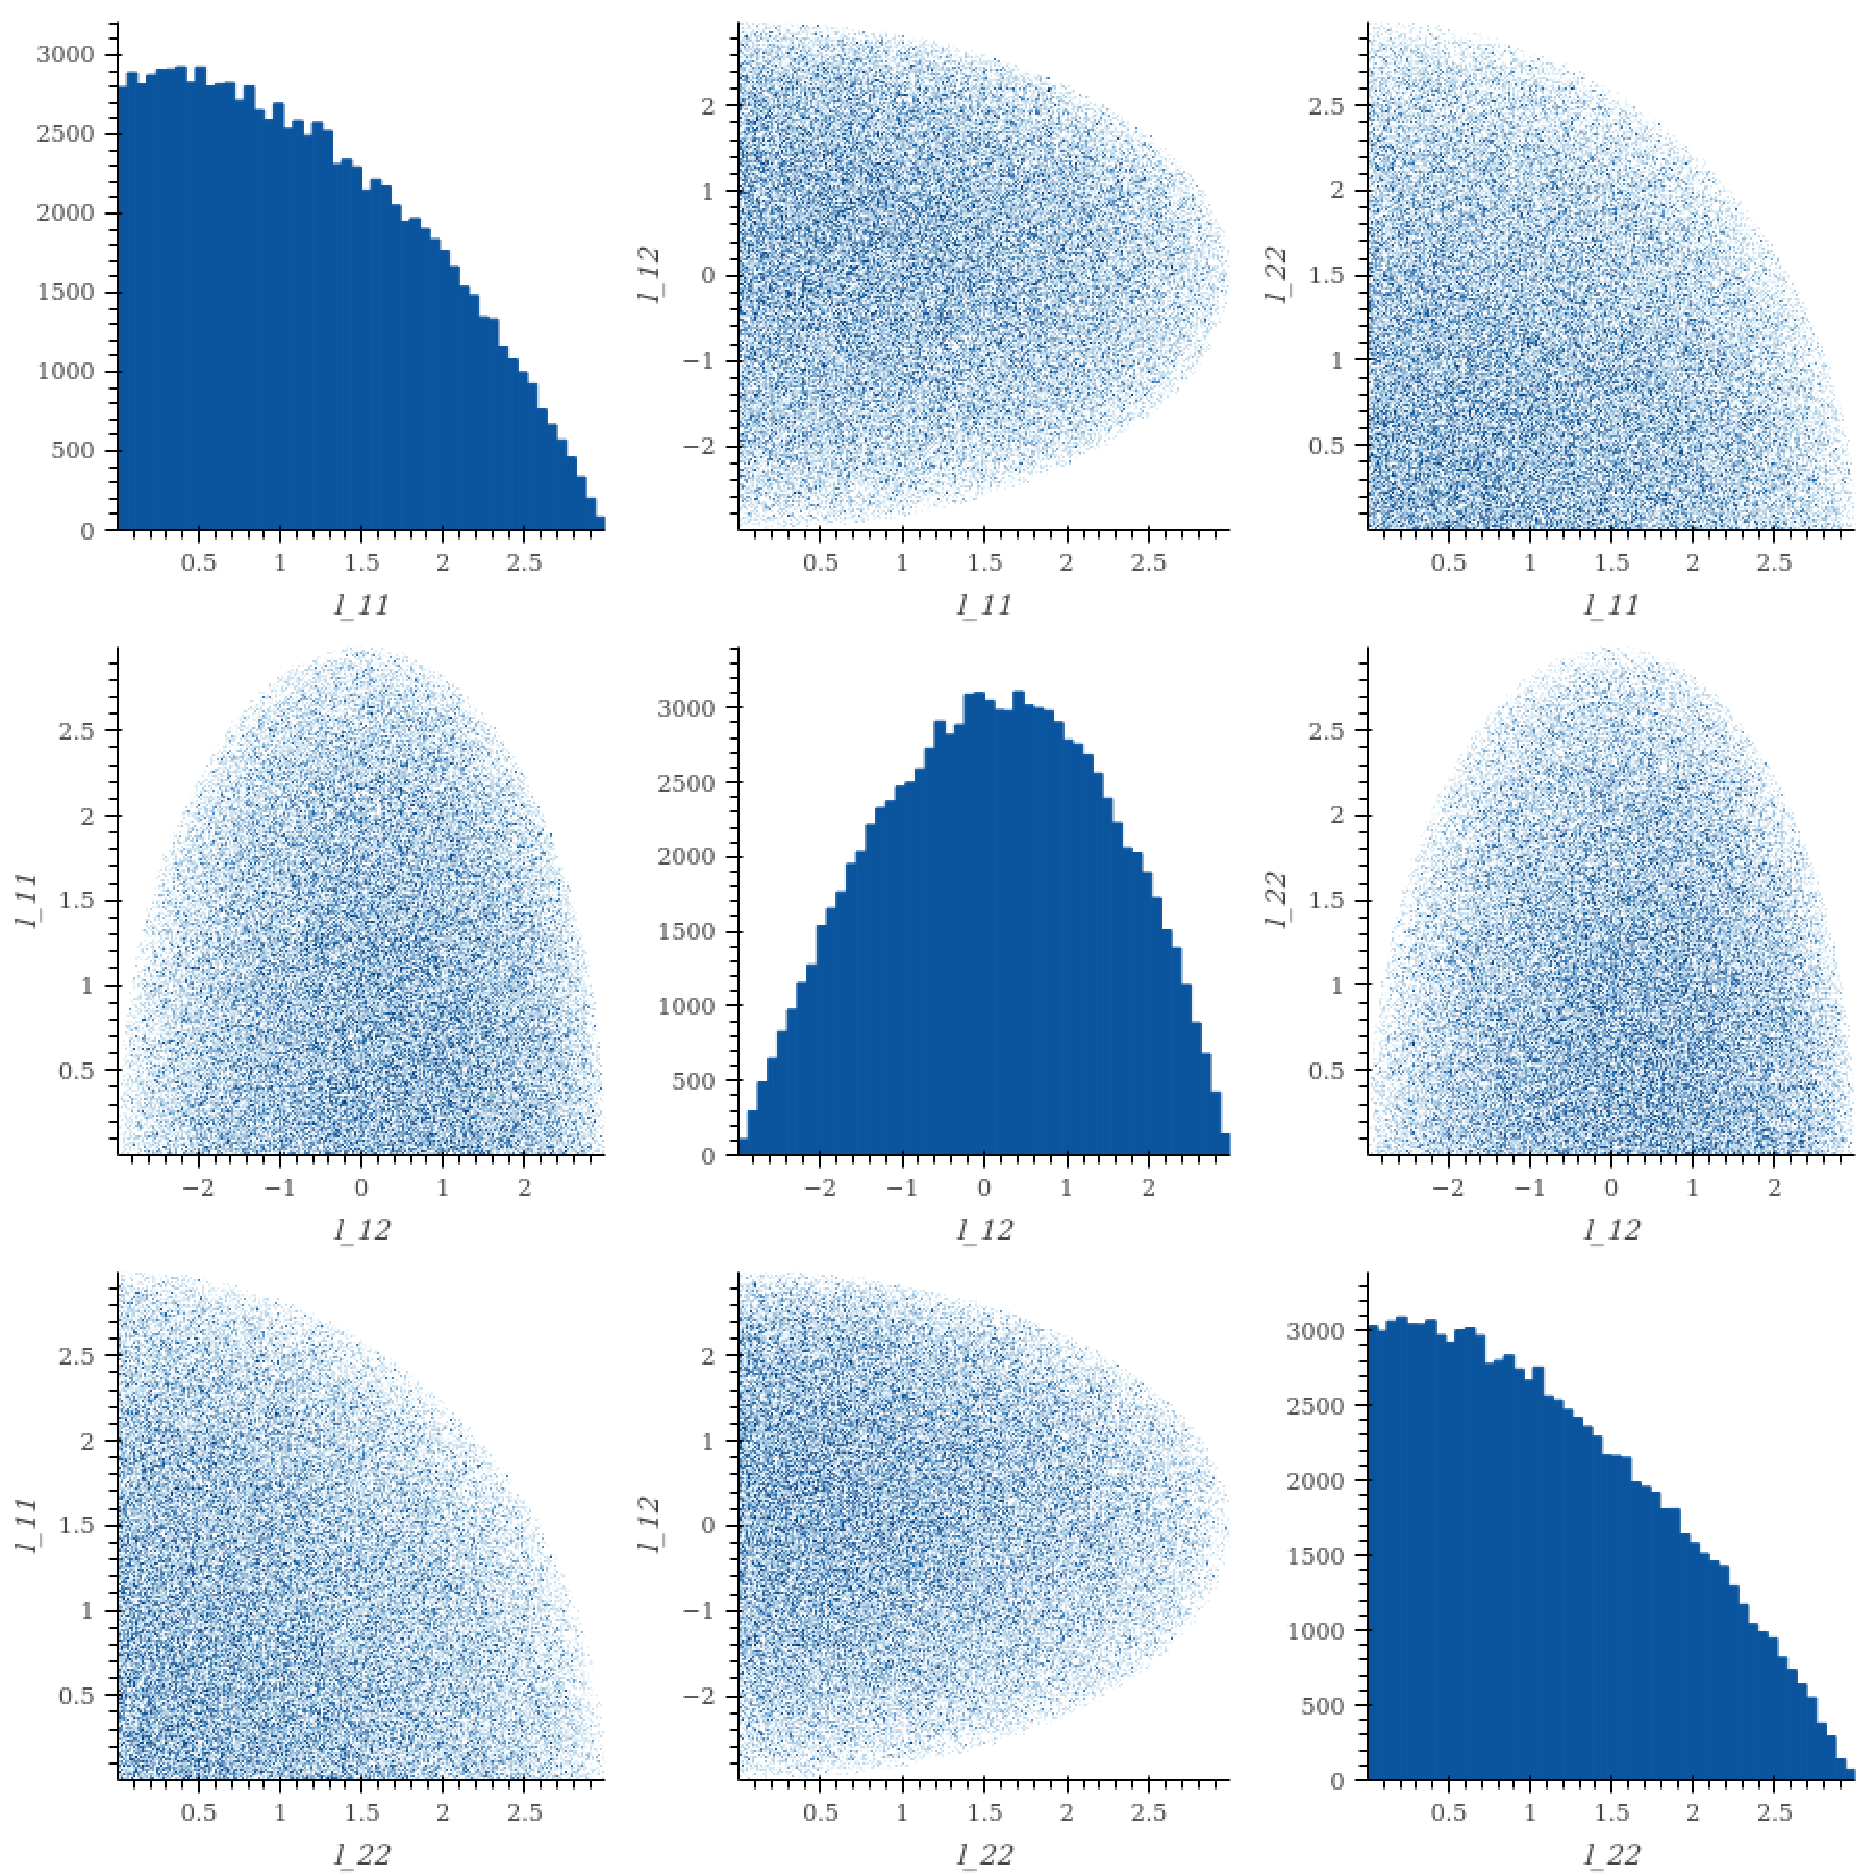
\includegraphics[width=\textwidth]{images/constraind_diffusion_rejection/pairplots/spd_uniform_ll.pdf}
		\caption{Plots of the univariate marginal and pairwise bivariate distributions of \num{1e5} samples from the uniform distribution in \(\c{S}_{++}^2\).}
		\label{fig:app_pairplots_robot_reflected_ellips}
	\end{subfigure}
	\hfill
	\begin{subfigure}[t]{0.45\textwidth}
		\centering
		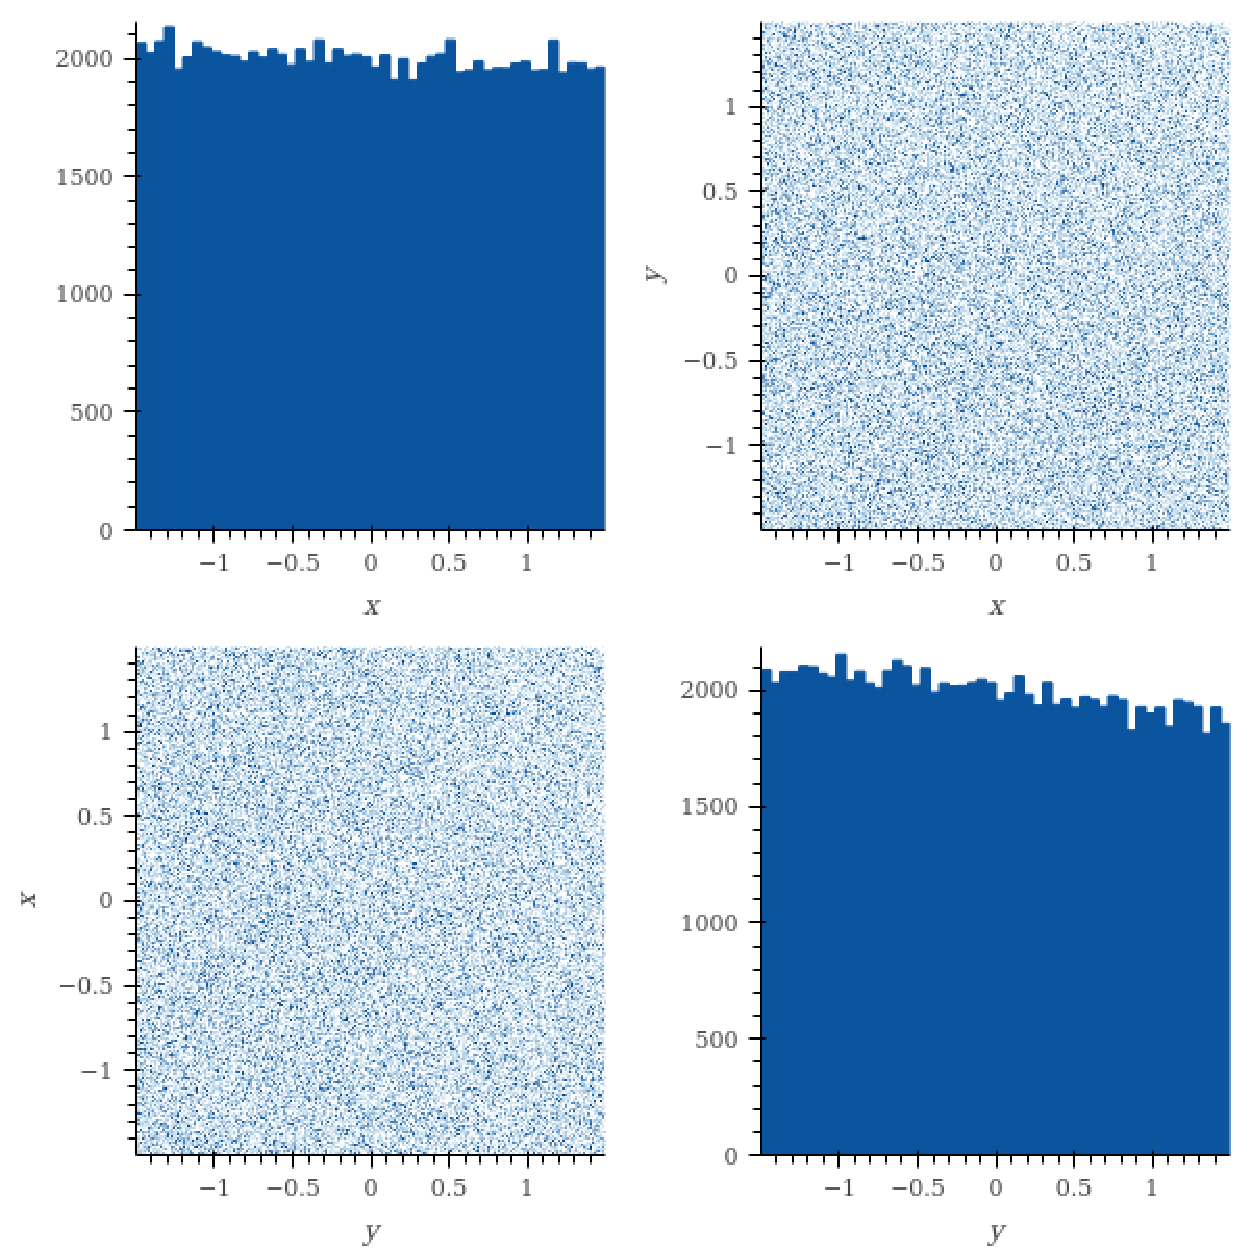
\includegraphics[width=\textwidth]{images/constraind_diffusion_rejection/pairplots/spd_uniform_xy.pdf}
		\caption{Plots of the univariate marginal and pairwise bivariate distributions of \num{1e5} samples from the uniform distribution in \(\R^2\).}
		\label{fig:app_pairplots_robot_reflected_location}
	\end{subfigure}
	\caption{Visualisation of the uniform distribution in \(\c{S}_{++}^2\times\R^2\) using univariate marginal and pairwise bivariate plots.}
	\label{fig:app_pairplots_robot_uniform}
\end{figure}

\subsection{Conformational Modelling of Protein Backbones}
\label{sec:app_loop_pairplots}

The following univariate marginal and pairwise bivariate plots visualise the distribution of different samples in \begin{enumerate*}[label=(\roman*)] \item the polytope \(\mathbb{P}\subset\R^3\) and \item the torus \(\mathbb{T}^4\) \end{enumerate*} used to parametrise the conformations of a polypeptide chain of length \(N=6\) with coinciding endpoints.
We refer to \cite{han2006inverse} for full detail on the reparametrisation and to \cite{fishman2023diffusion} for a full description of the dataset.

\subsubsection{Visualisation of samples from the data distribution}

\begin{figure}[H]
	\centering
	\begin{subfigure}[t]{0.45\textwidth}
		\centering
		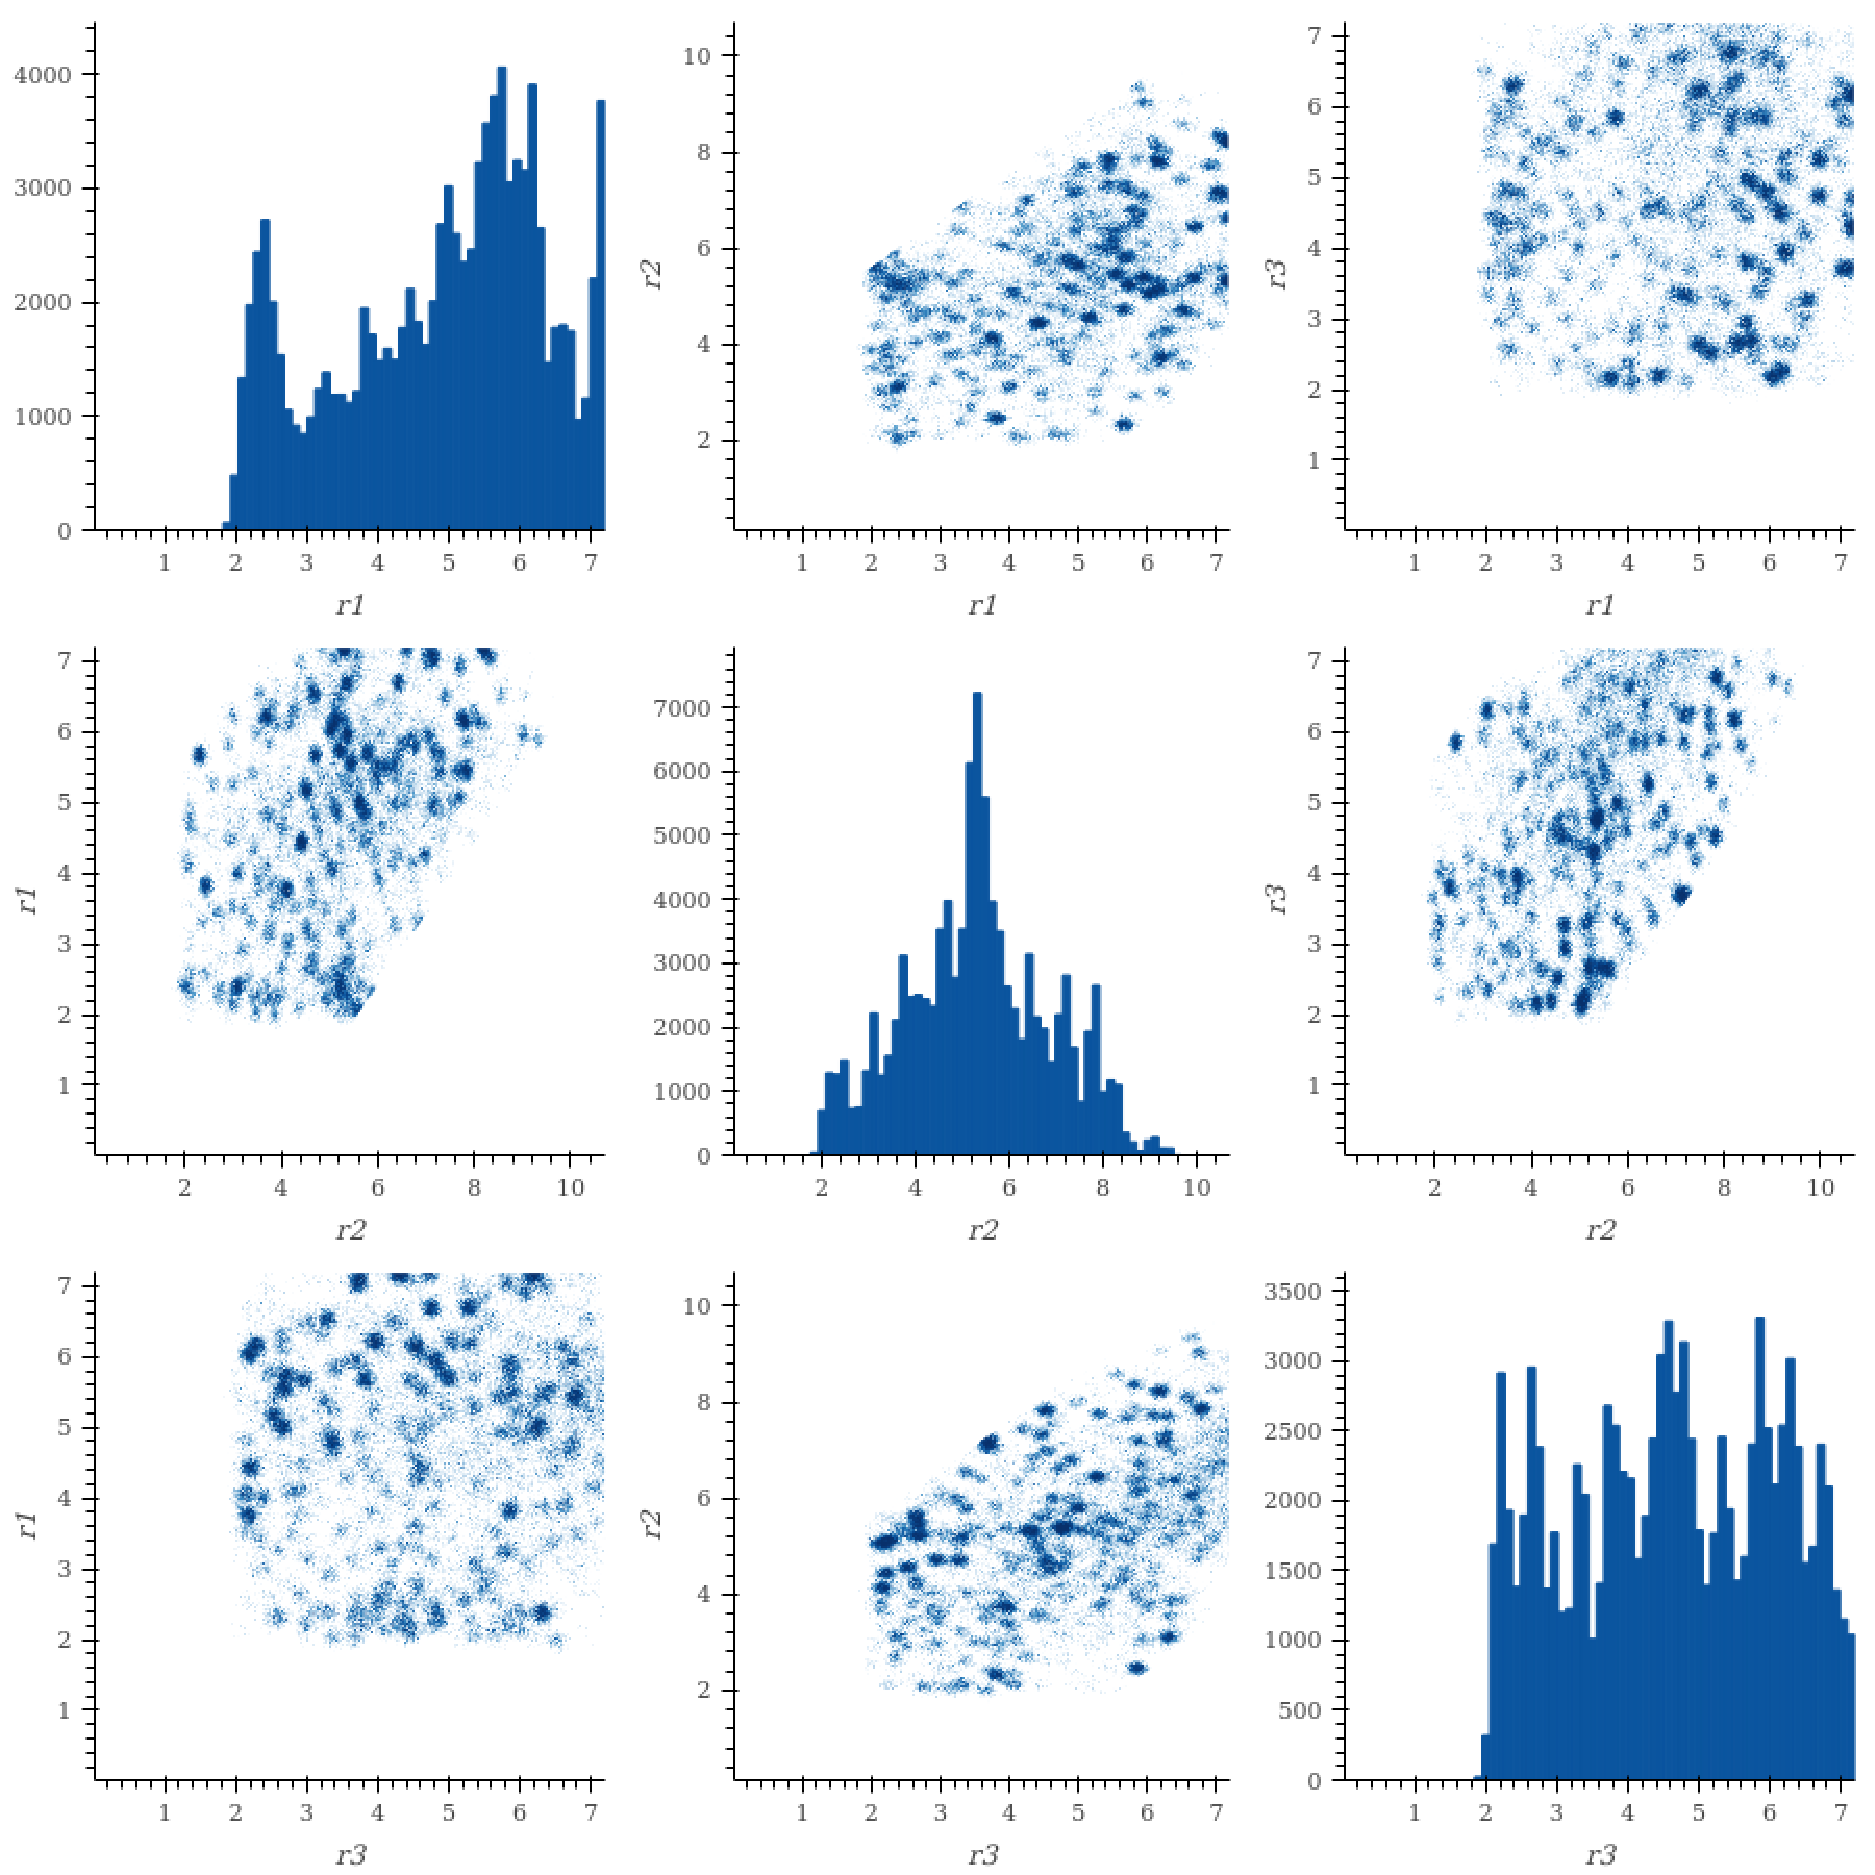
\includegraphics[width=\textwidth]{images/constraind_diffusion_rejection/pairplots/loops_polytope_data.pdf}
		\caption{Plots of the univariate marginal and pairwise bivariate distributions of \num{1e5} samples from the data distribution in \(\mathbb{P}\subset\R^3\).}
		\label{fig:app_pairplots_loop_polytope_data}
	\end{subfigure}
	\hfill
	\begin{subfigure}[t]{0.45\textwidth}
		\centering
		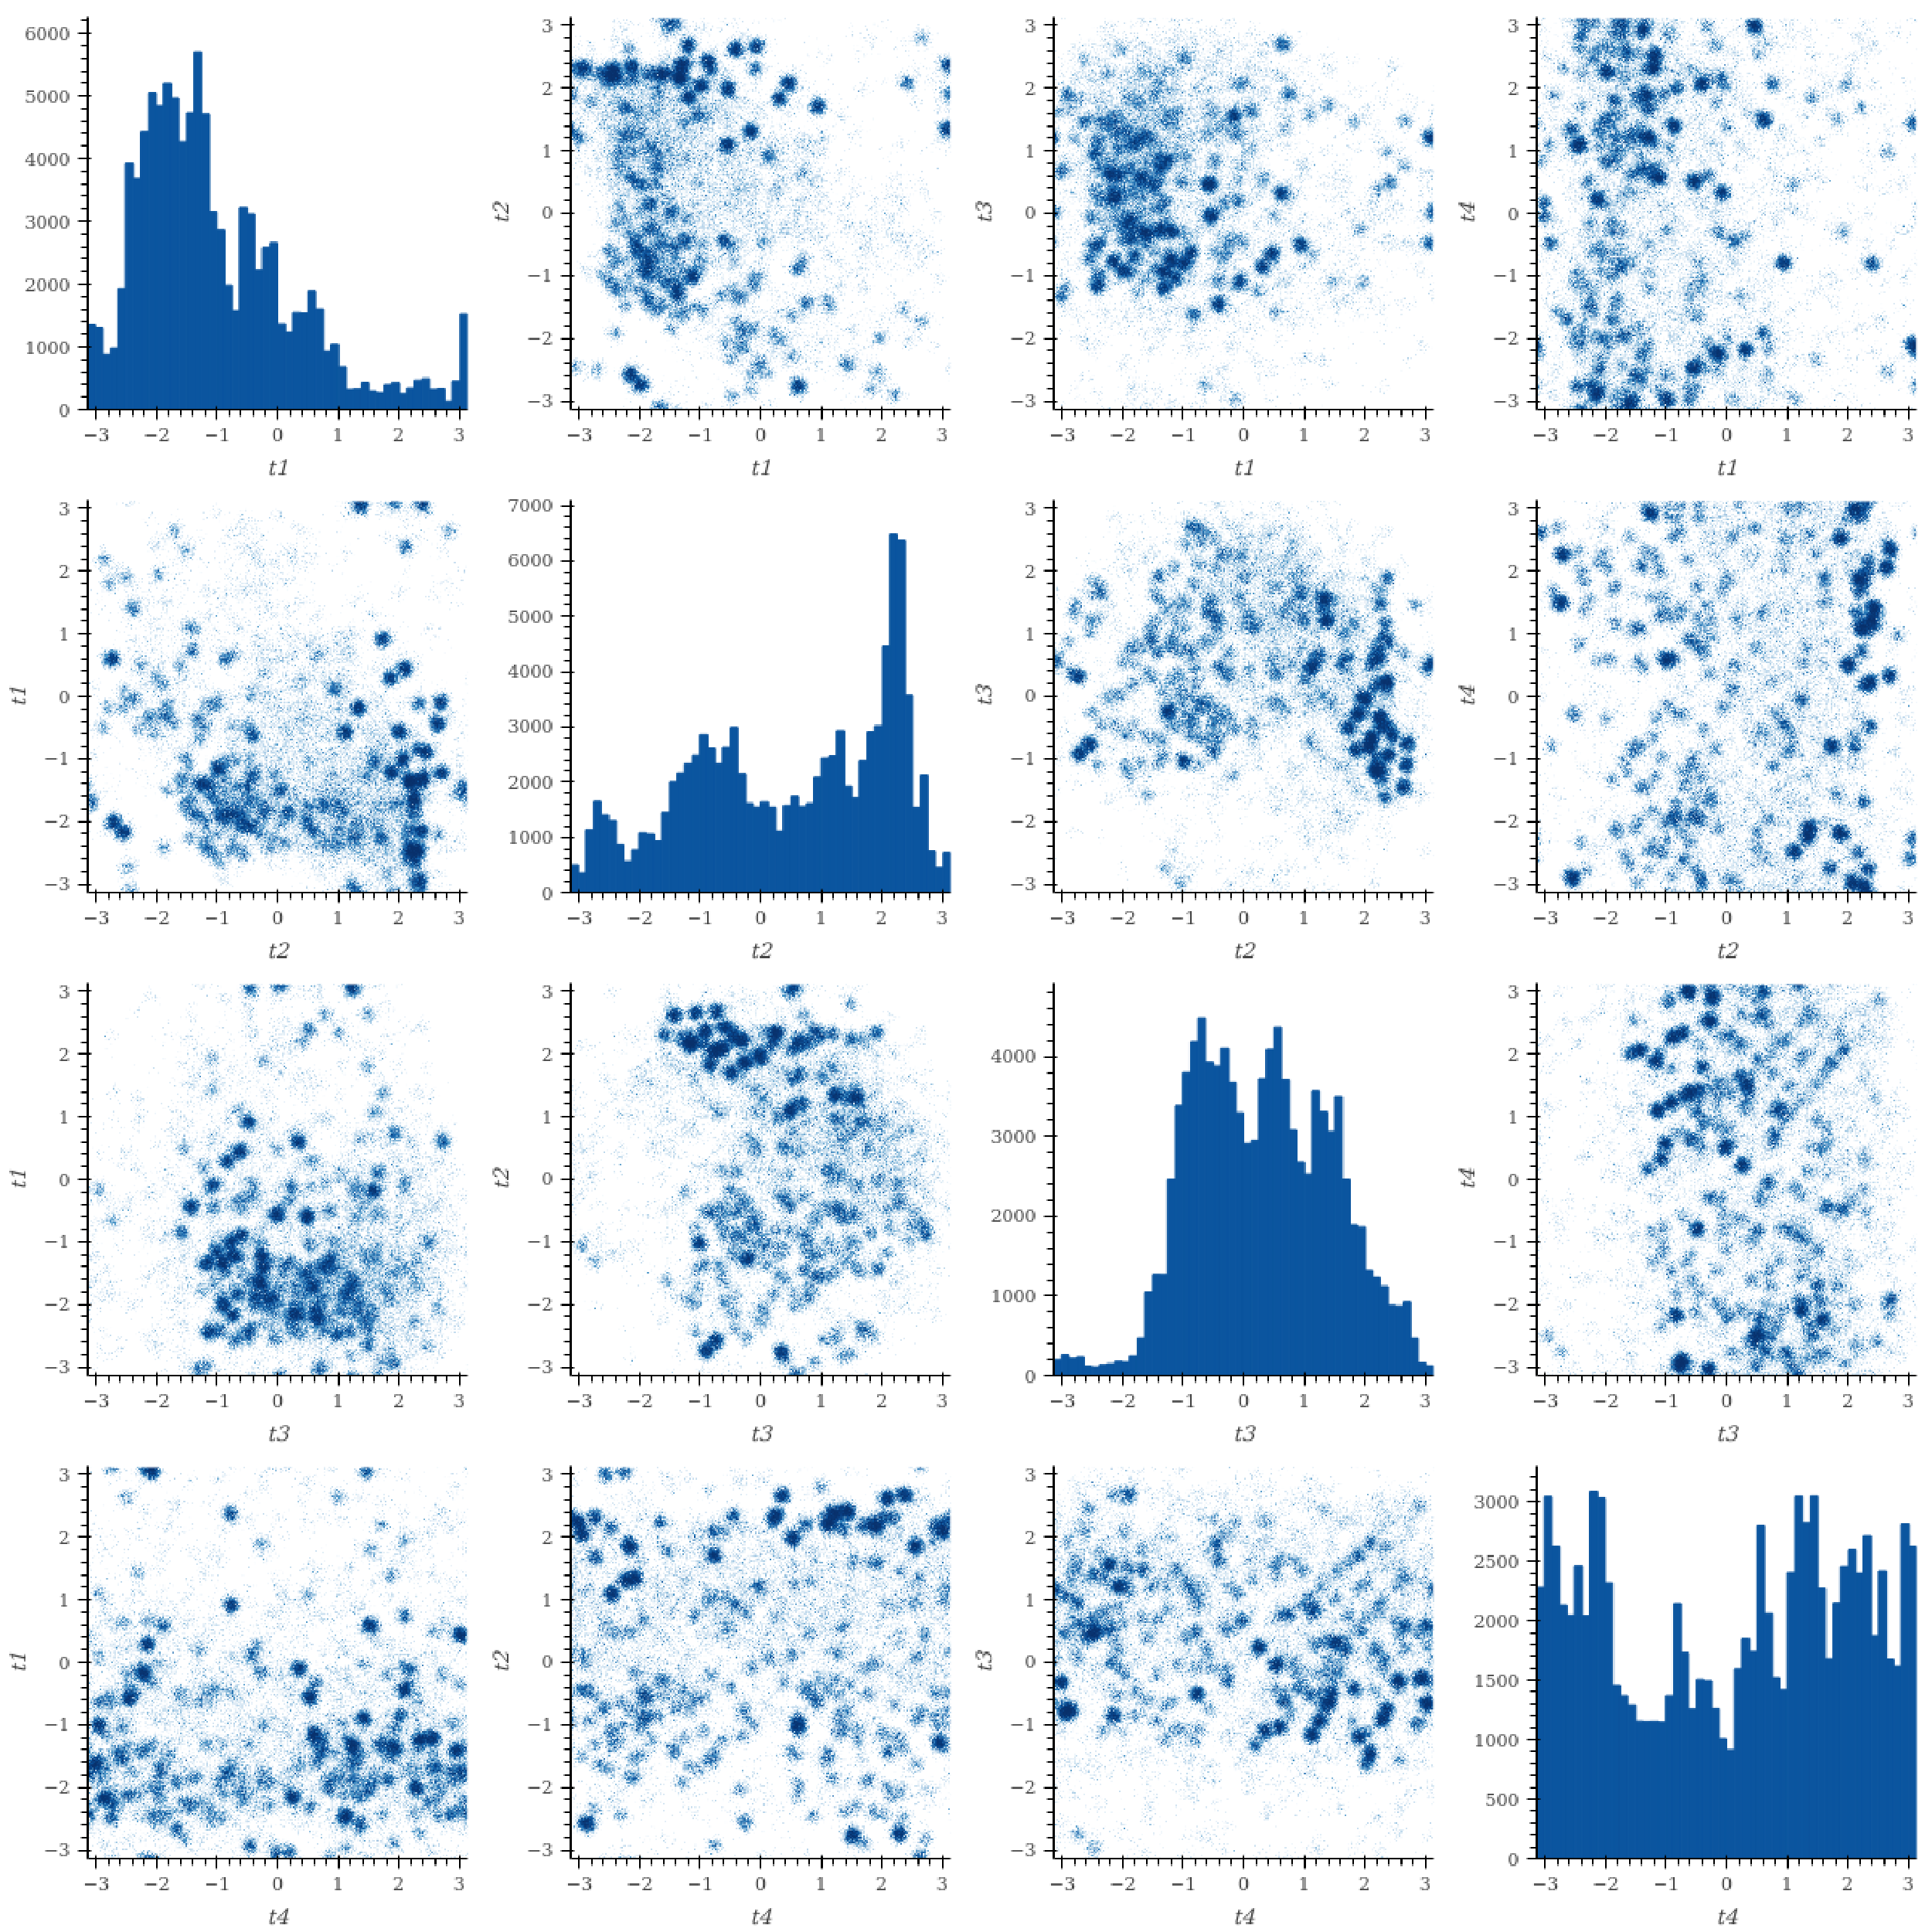
\includegraphics[width=\textwidth]{images/constraind_diffusion_rejection/pairplots/loops_torus_data.pdf}
		\caption{Plots of the univariate marginal and pairwise bivariate distributions of \num{1e5} samples from the data distribution in \(\mathbb{T}^4\).}
		\label{fig:app_pairplots_loop_torus_data}
	\end{subfigure}
	\caption{Visualisation of the data distribution in \(\mathbb{P}\subset\R^3\times\mathbb{T}^4\) using univariate marginal and pairwise bivariate plots.}
	\label{fig:app_pairplots_loop_data}
\end{figure}

\subsubsection{Visualisation of samples from our Metropolis sampling-based diffusion model}

\begin{figure}[H]
	\centering
	\begin{subfigure}[t]{0.45\textwidth}
		\centering
		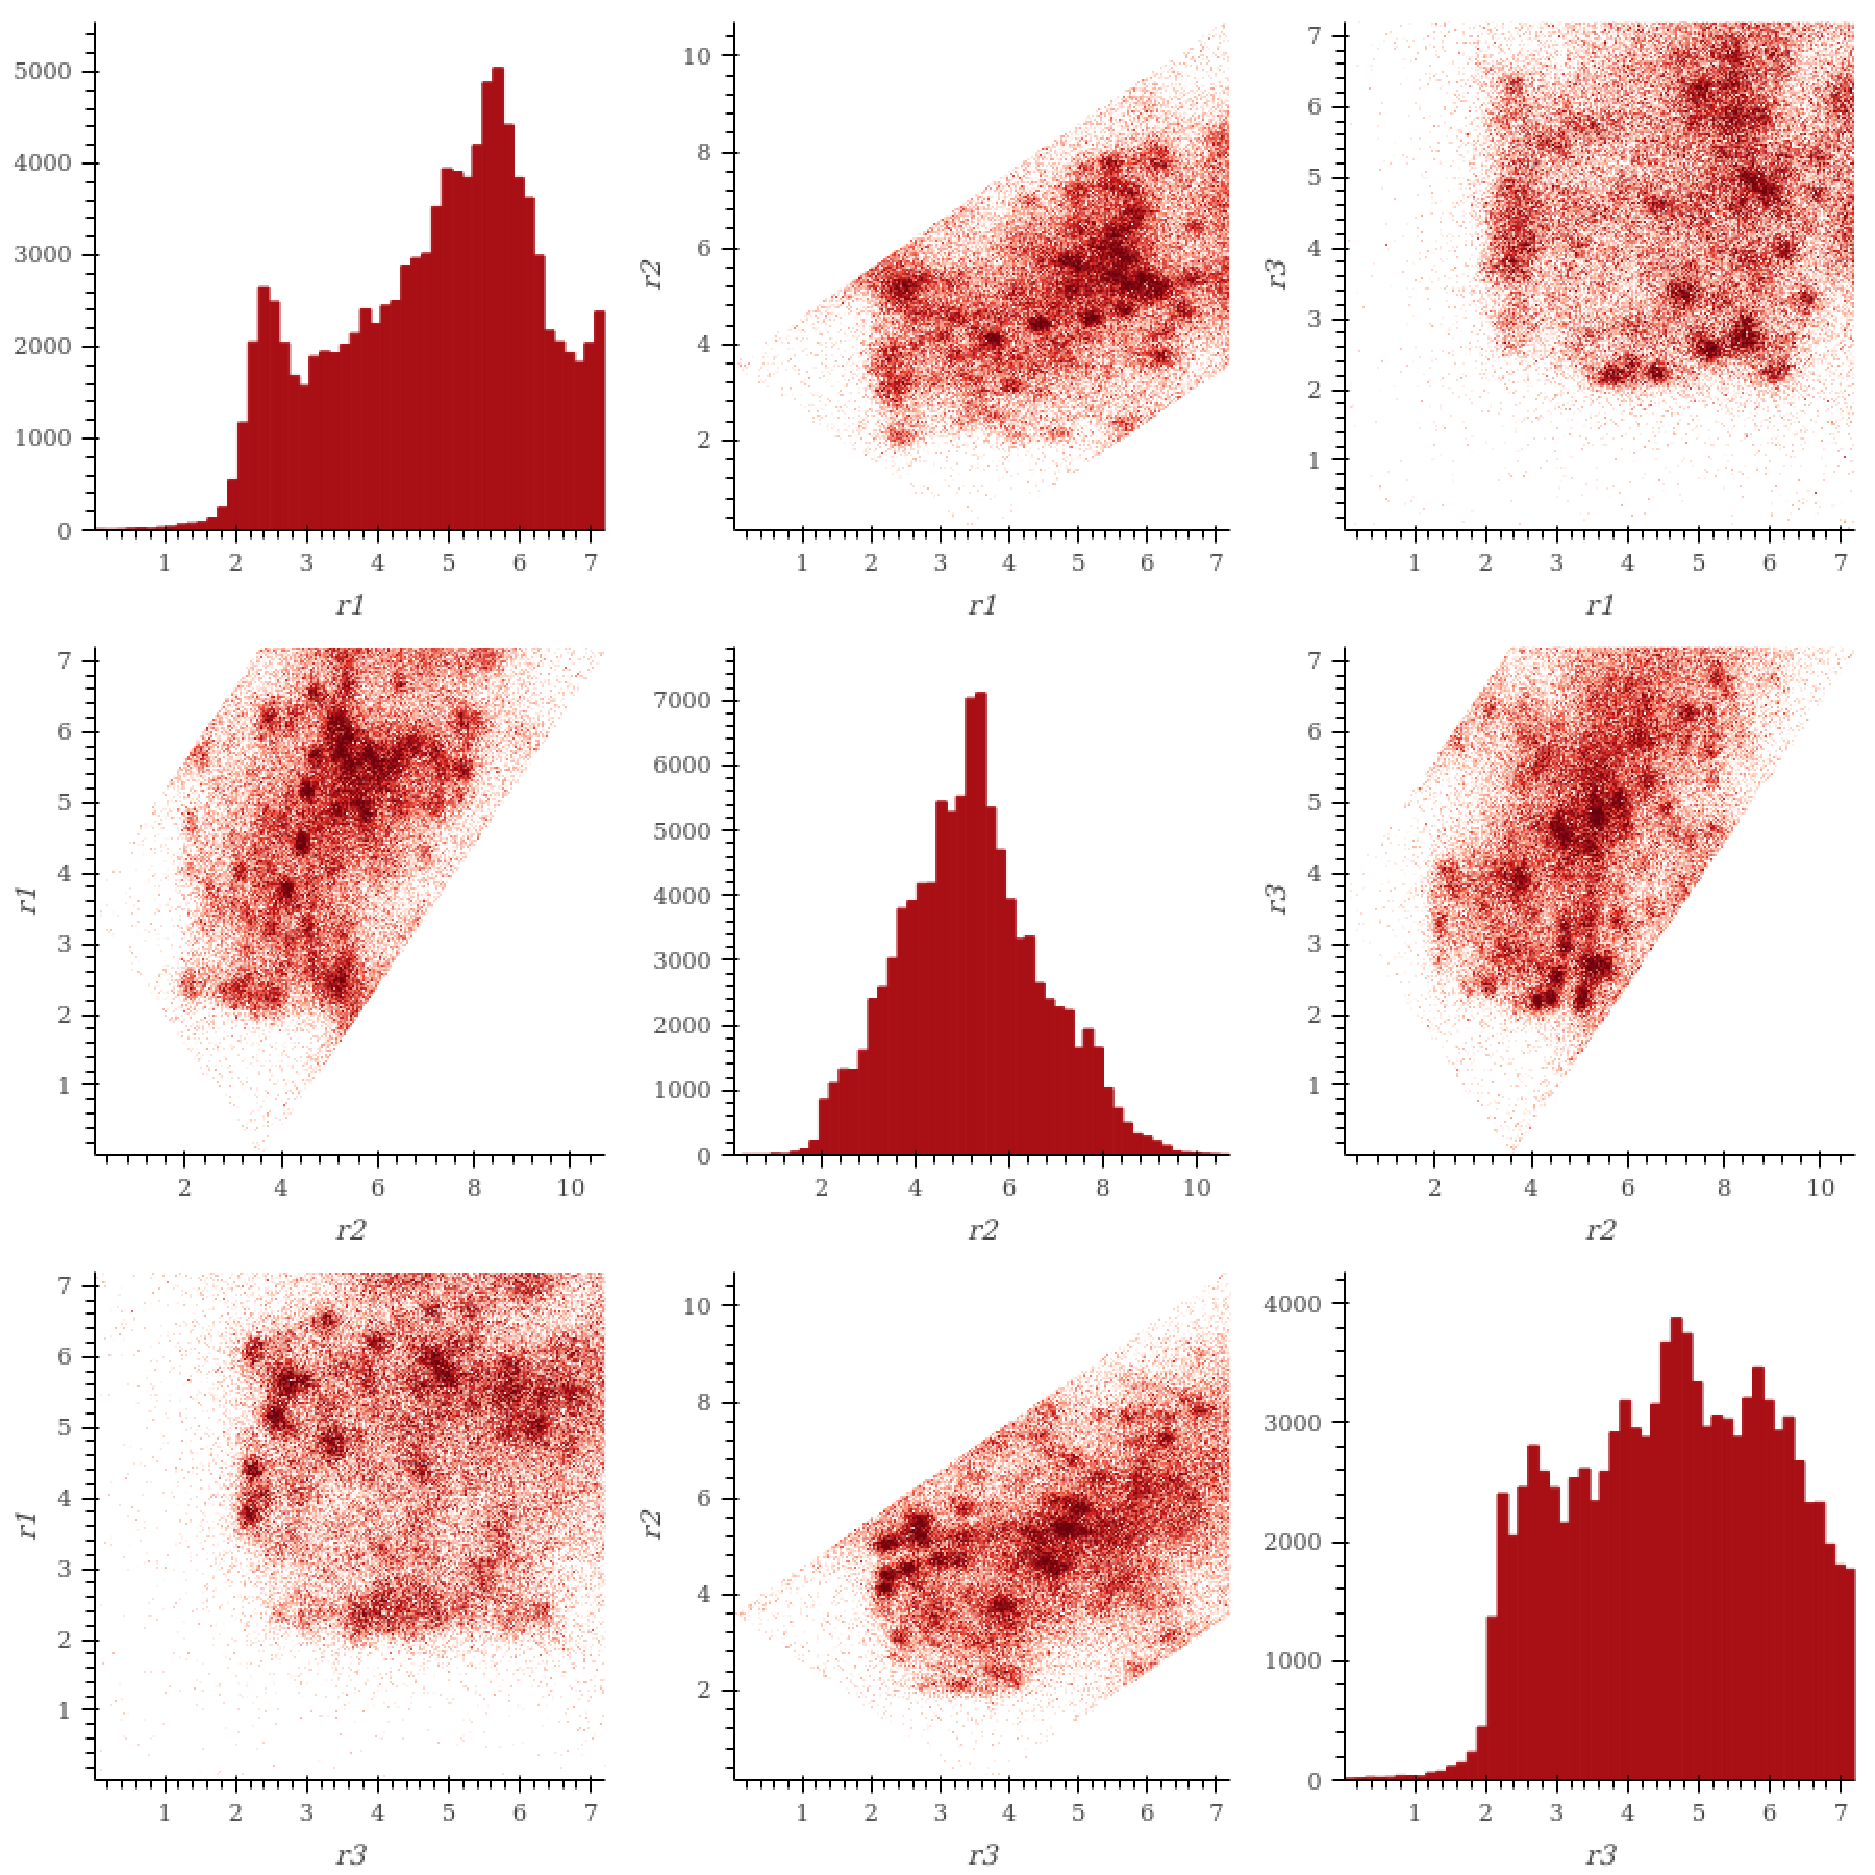
\includegraphics[width=\textwidth]{images/constraind_diffusion_rejection/pairplots/loops_polytope_rejection.pdf}
		\caption{Plots of the univariate marginal and pairwise bivariate distributions of \num{1e5} samples from our Metropolis model in \(\mathbb{P}\subset\R^3\).}
		\label{fig:app_pairplots_loop_polytope_rejection}
	\end{subfigure}
	\hfill
	\begin{subfigure}[t]{0.45\textwidth}
		\centering
		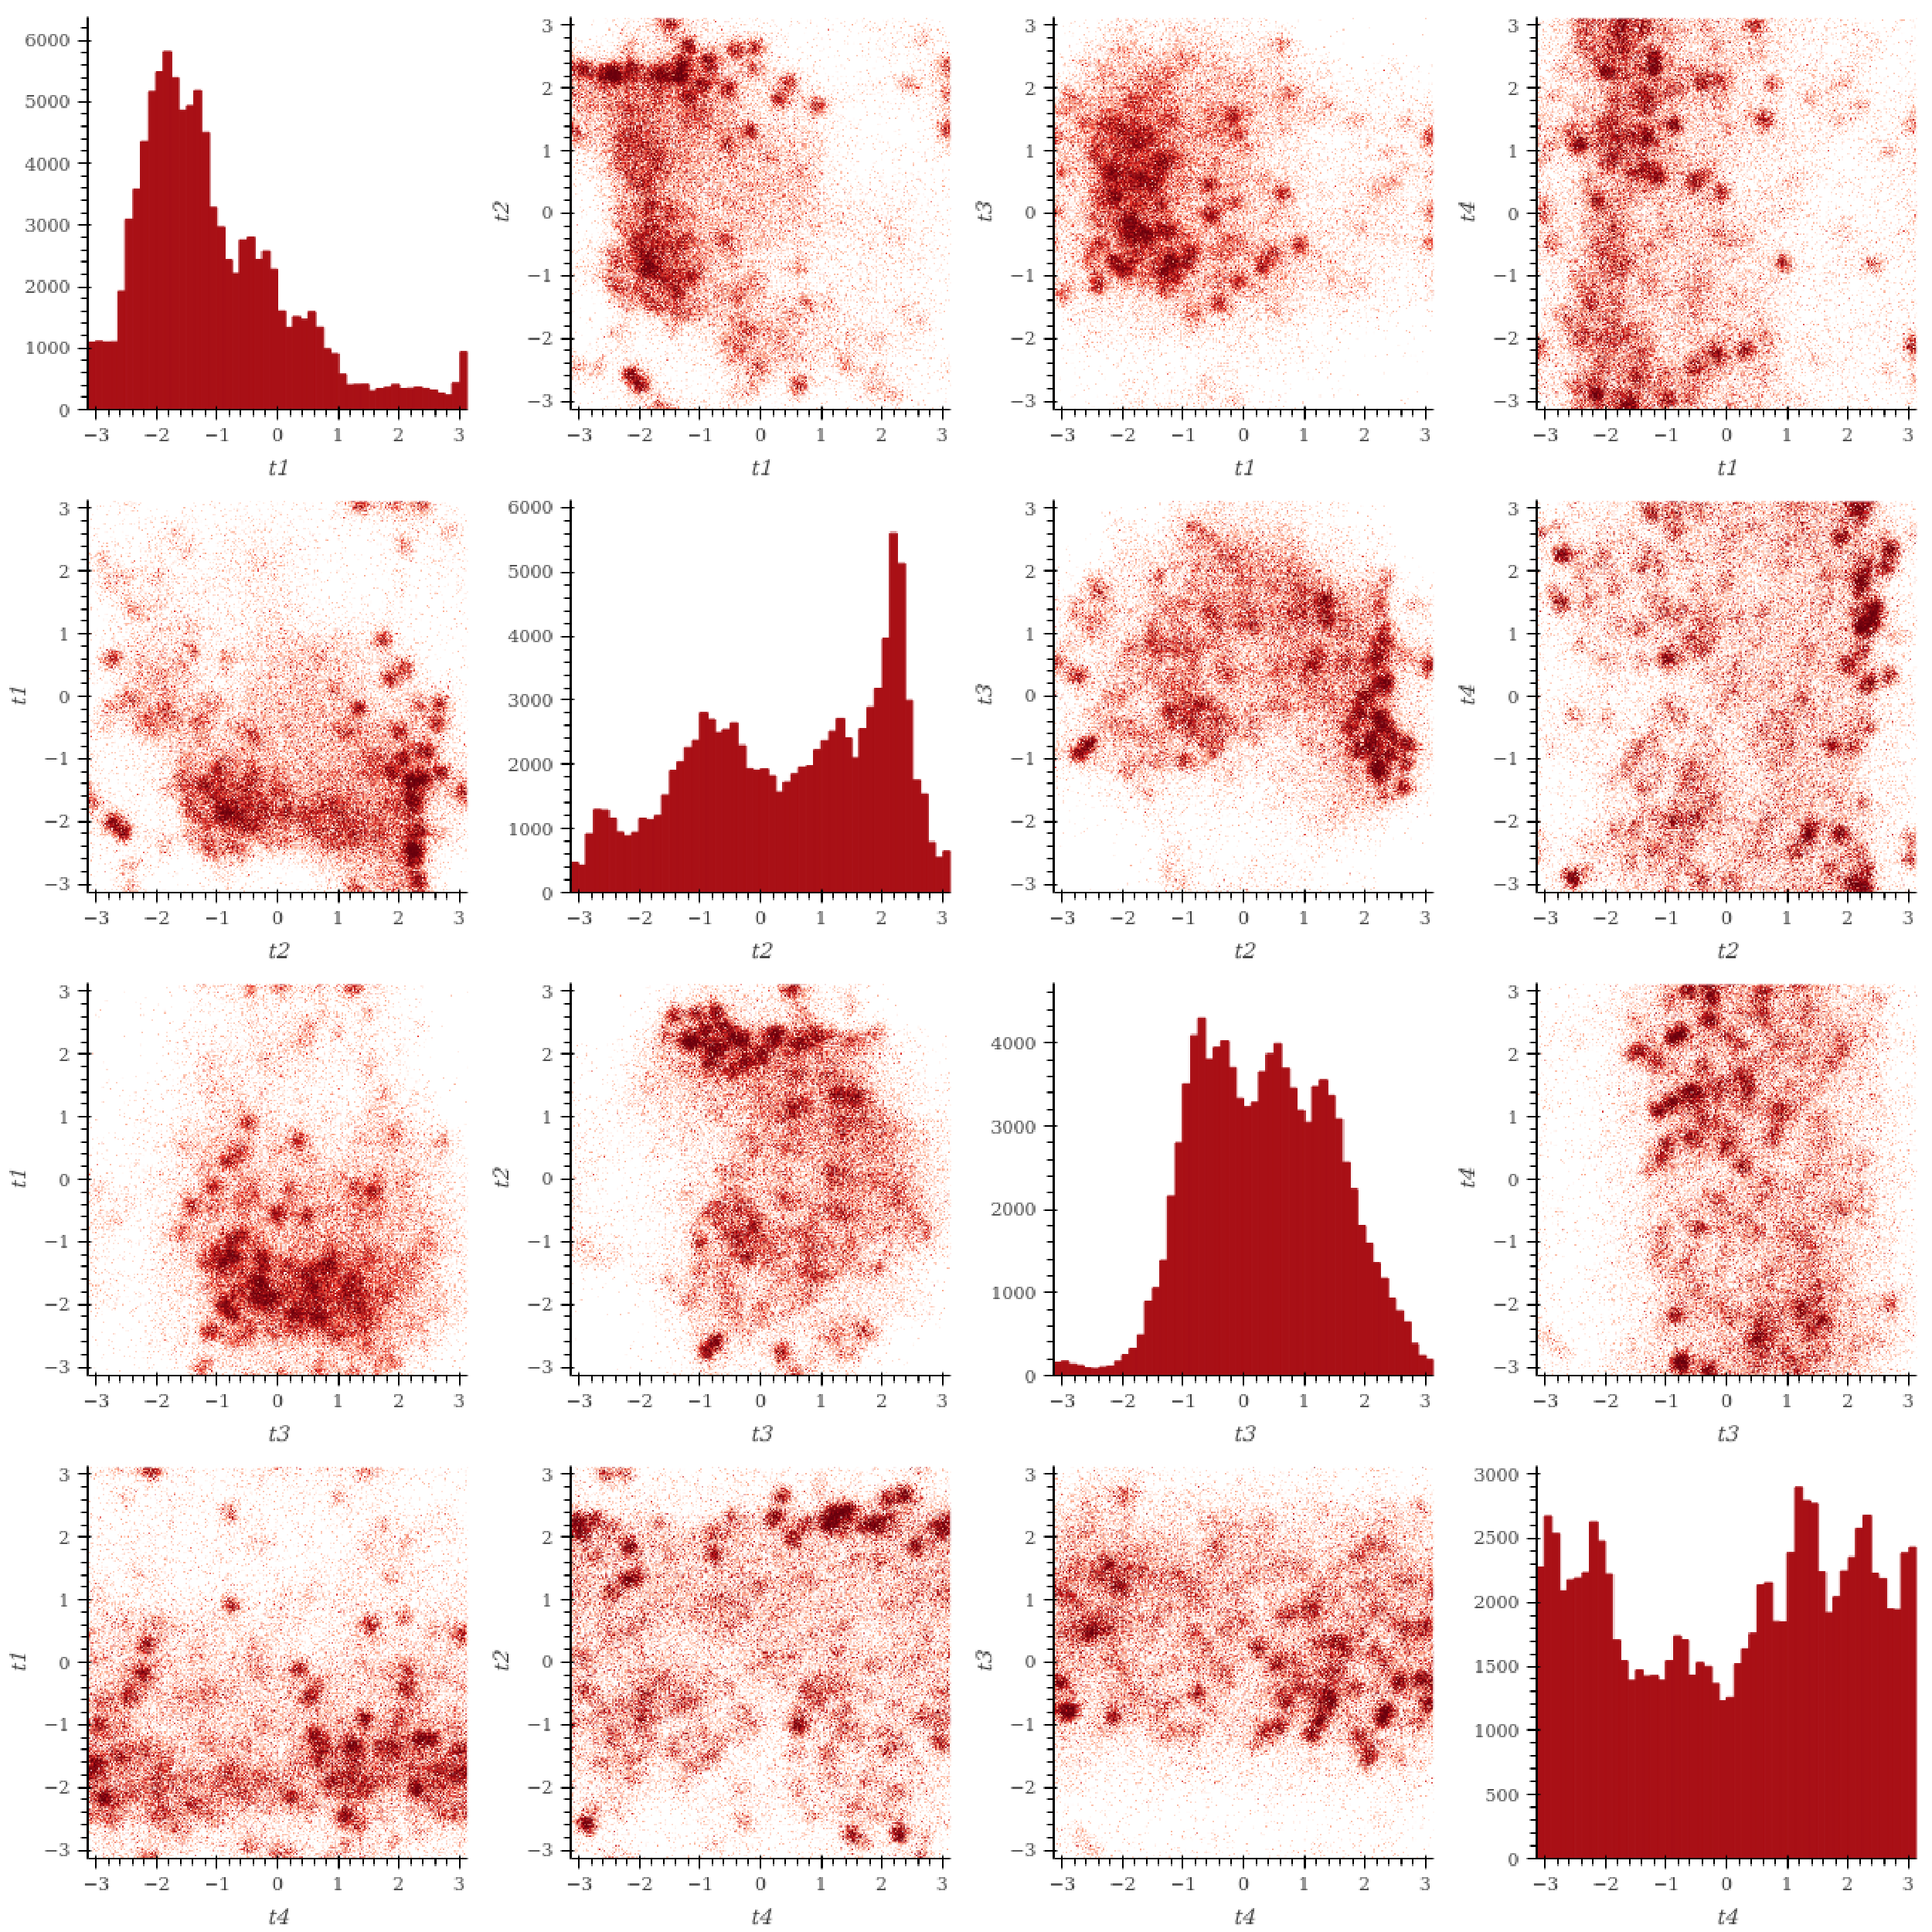
\includegraphics[width=\textwidth]{images/constraind_diffusion_rejection/pairplots/loops_torus_rejection.pdf}
		\caption{Plots of the univariate marginal and pairwise bivariate distributions of \num{1e5} samples from our Metropolis model in \(\mathbb{T}^4\).}
		\label{fig:app_pairplots_loop_torus_rejection}
	\end{subfigure}
	\caption{Visualisation of the distribution learned by our Metropolis model in \(\mathbb{P}\subset\R^3\times\mathbb{T}^4\) using univariate marginal and pairwise bivariate plots.}
	\label{fig:app_pairplots_loop_rejection}
\end{figure}

\subsubsection{Visualisation of samples from a reflected Brownian motion-based diffusion model}

\begin{figure}[H]
	\centering
	\begin{subfigure}[t]{0.45\textwidth}
		\centering
		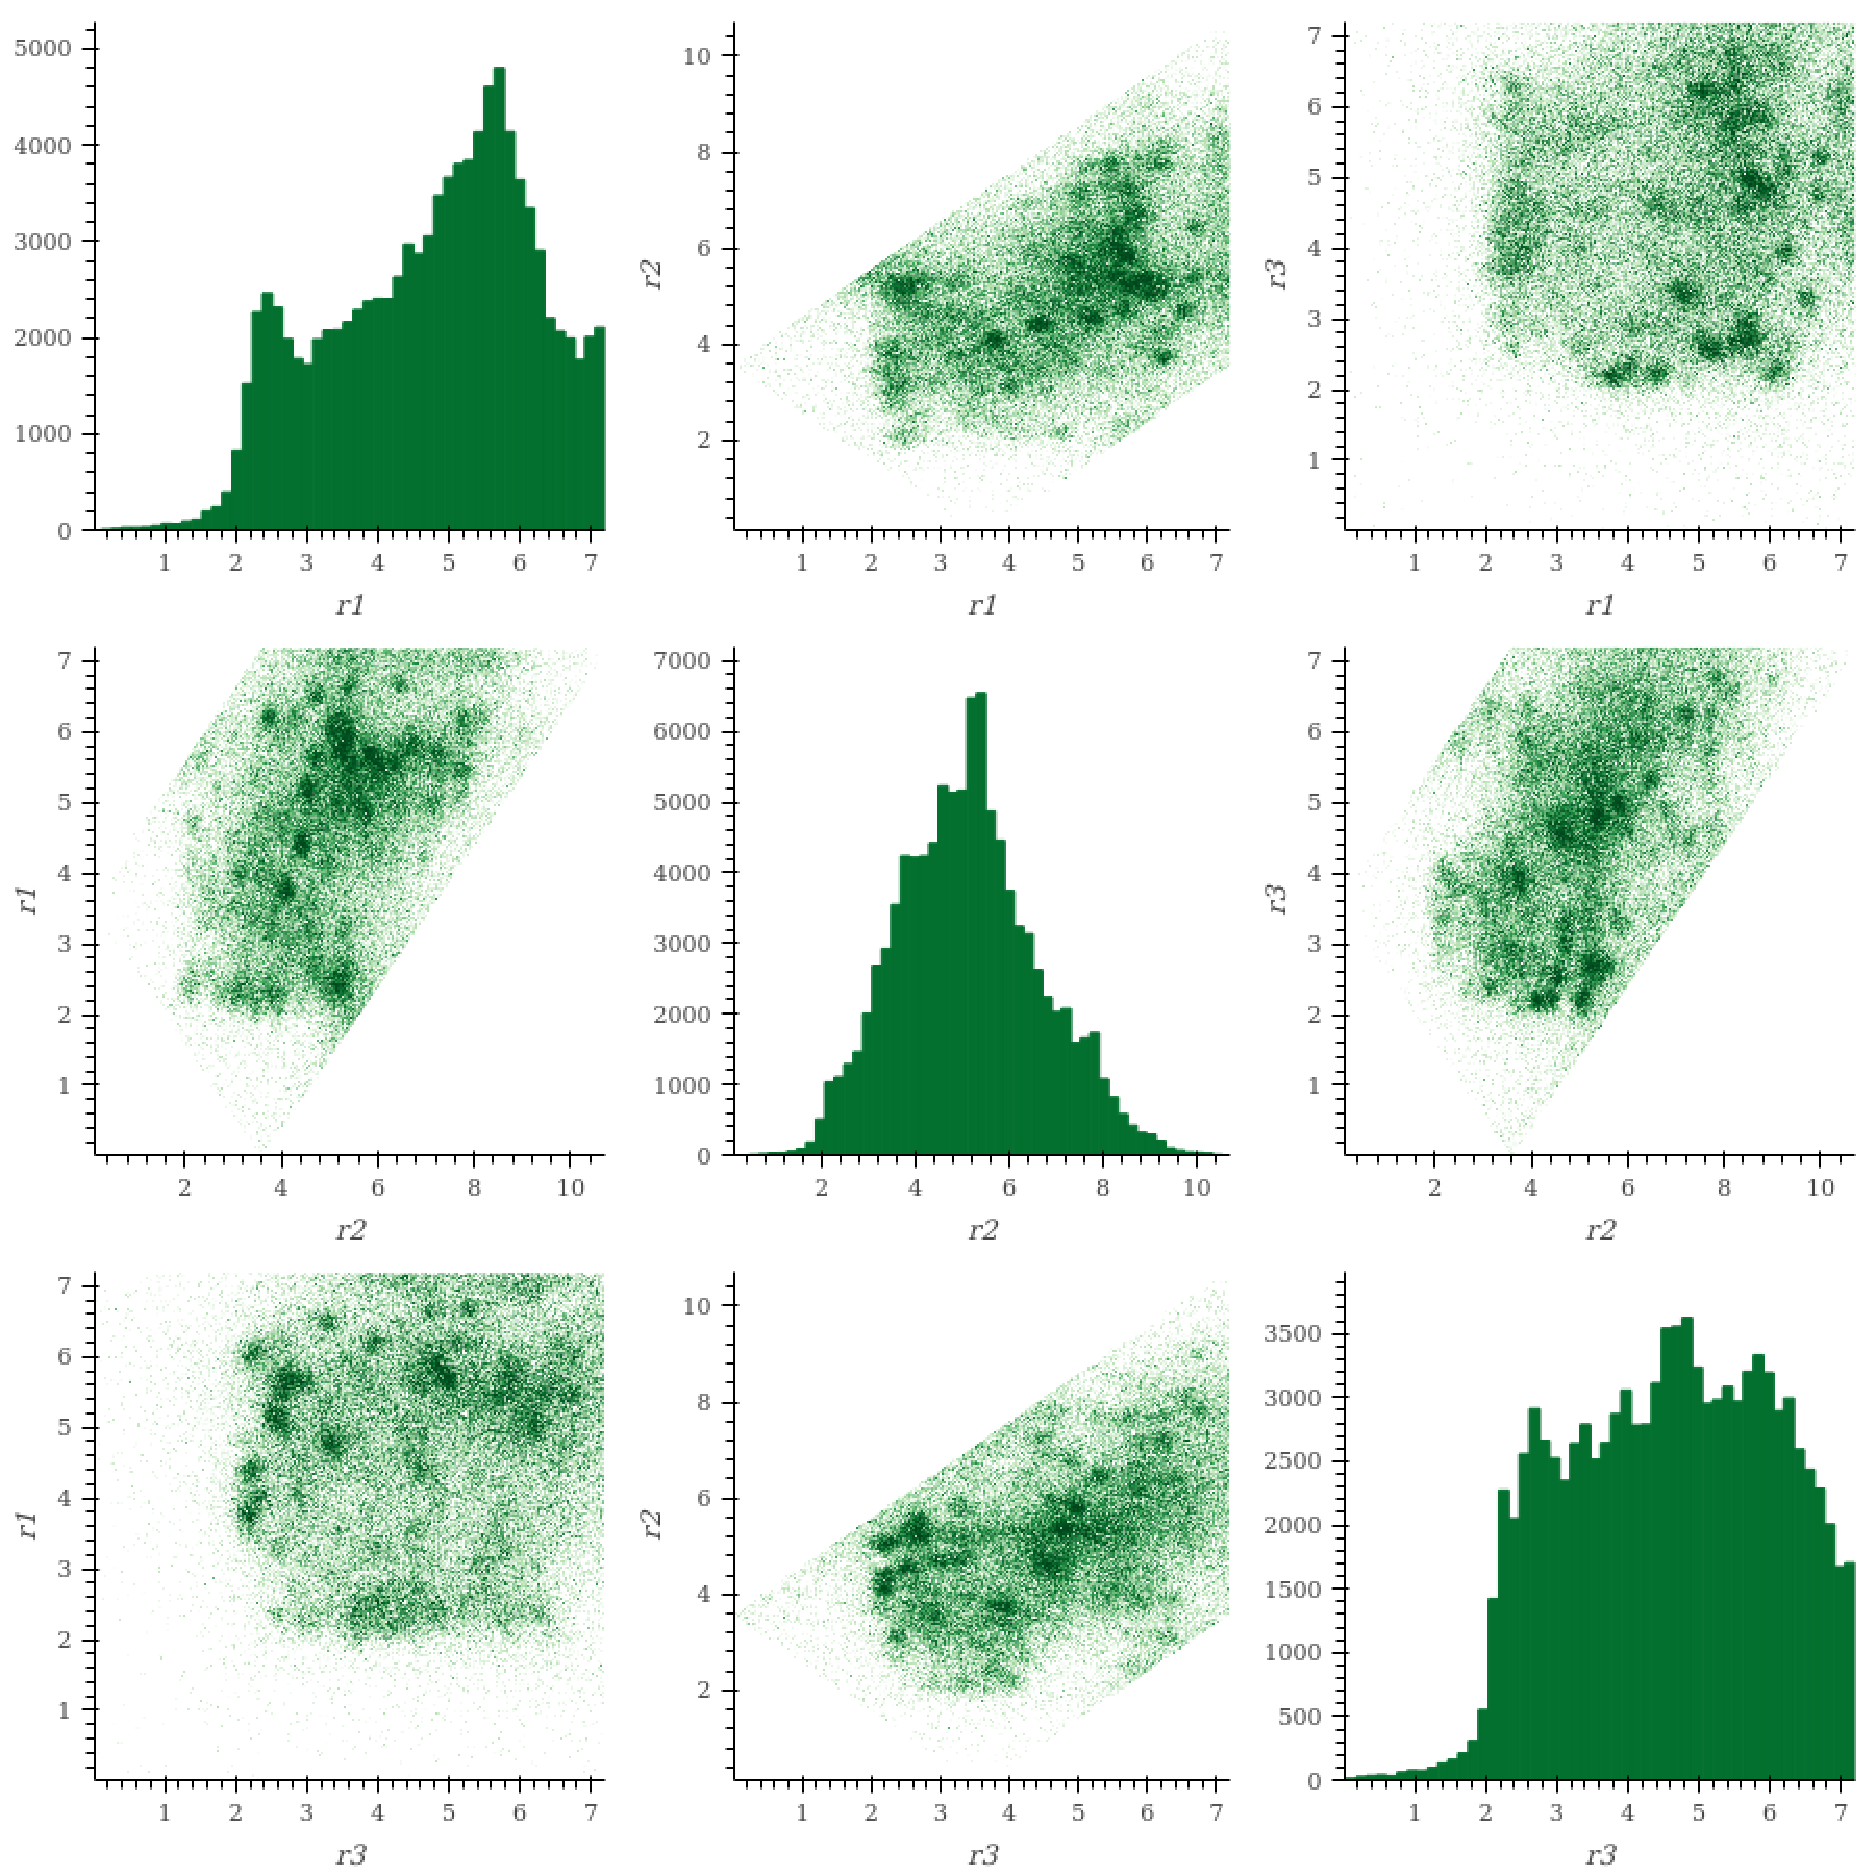
\includegraphics[width=\textwidth]{images/constraind_diffusion_rejection/pairplots/loops_polytope_reflection.pdf}
		\caption{Plots of the univariate marginal and pairwise bivariate distributions of \num{1e5} samples from a reflected Brownian motion-based diffusion model in \(\mathbb{P}\subset\R^3\).}
		\label{fig:app_pairplots_loop_polytope_reflected}
	\end{subfigure}
	\hfill
	\begin{subfigure}[t]{0.45\textwidth}
		\centering
		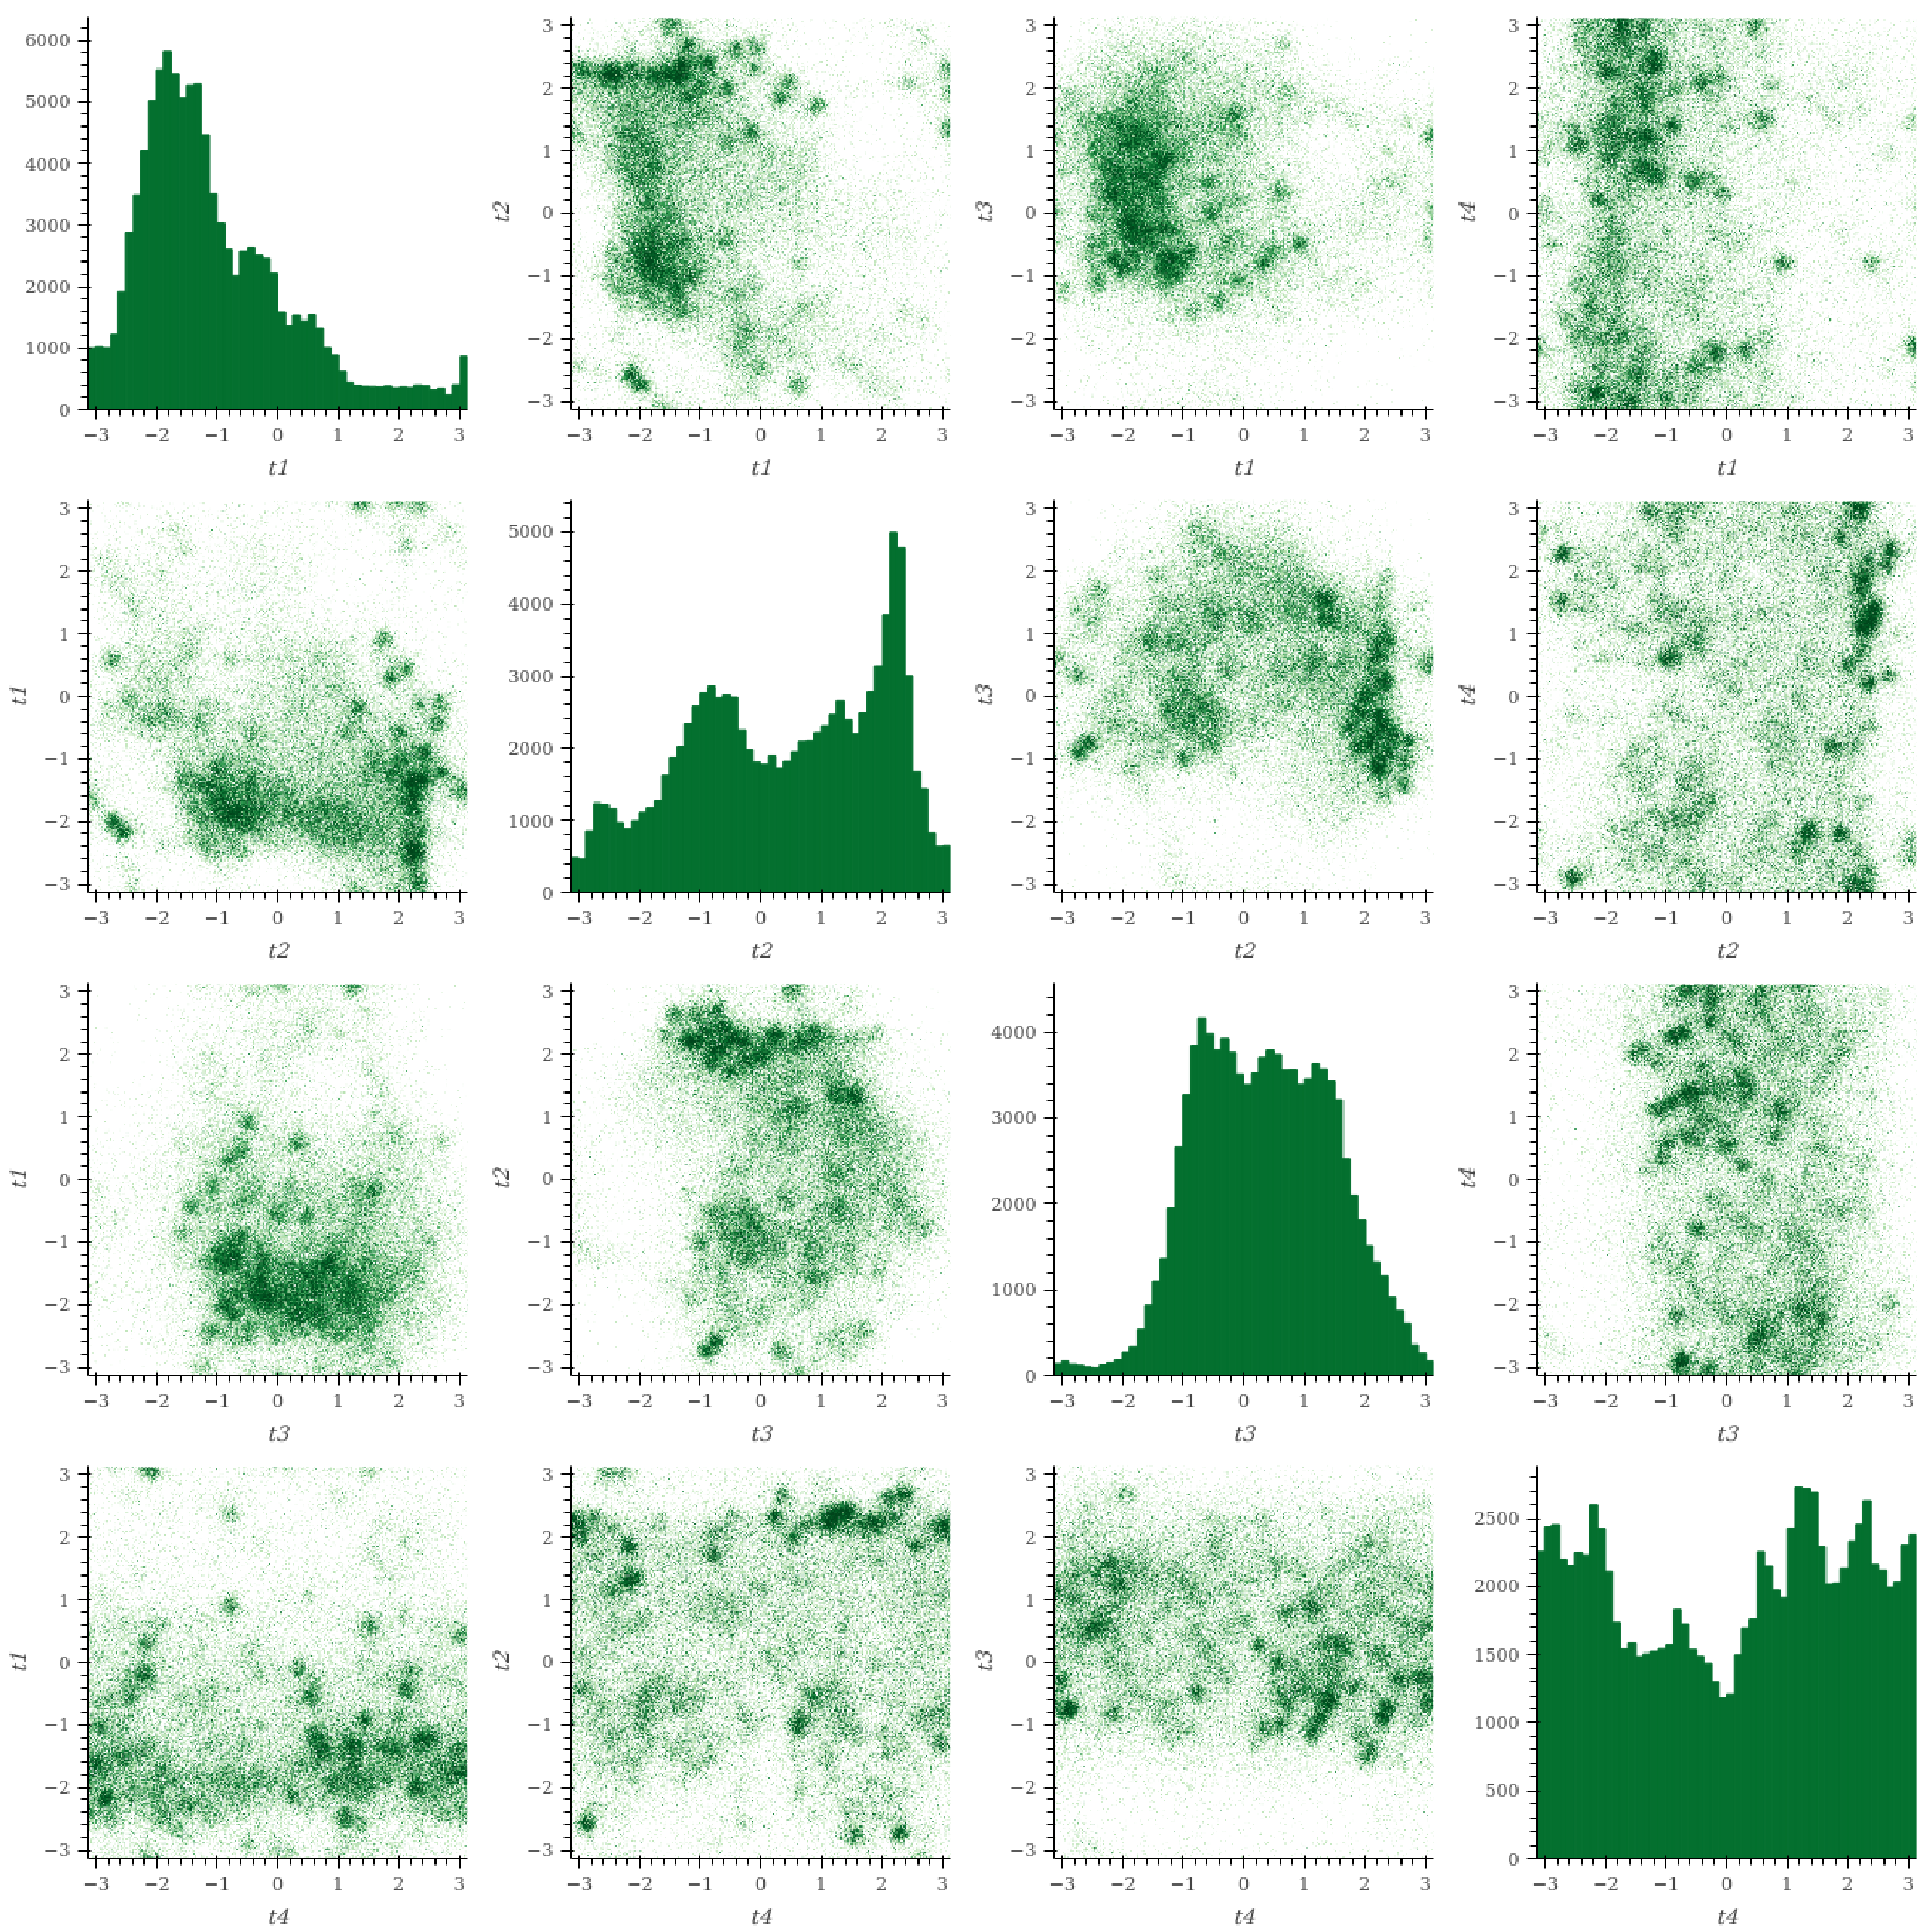
\includegraphics[width=\textwidth]{images/constraind_diffusion_rejection/pairplots/loops_torus_reflection.pdf}
		\caption{Plots of the univariate marginal and pairwise bivariate distributions of \num{1e5} samples from a reflected Brownian motion-based diffusion model in \(\mathbb{T}^4\).}
		\label{fig:app_pairplots_loop_torus_reflected}
	\end{subfigure}
	\caption{Visualisation of the distribution learned by a reflected Brownian motion-based diffusion model in \(\mathbb{P}\subset\R^3\times\mathbb{T}^4\) using univariate marginal and pairwise bivariate plots.}
	\label{fig:app_pairplots_loop_reflected}
\end{figure}

\subsubsection{Visualisation of samples from the uniform distribution}

\begin{figure}[H]
	\centering
	\begin{subfigure}[t]{0.45\textwidth}
		\centering
		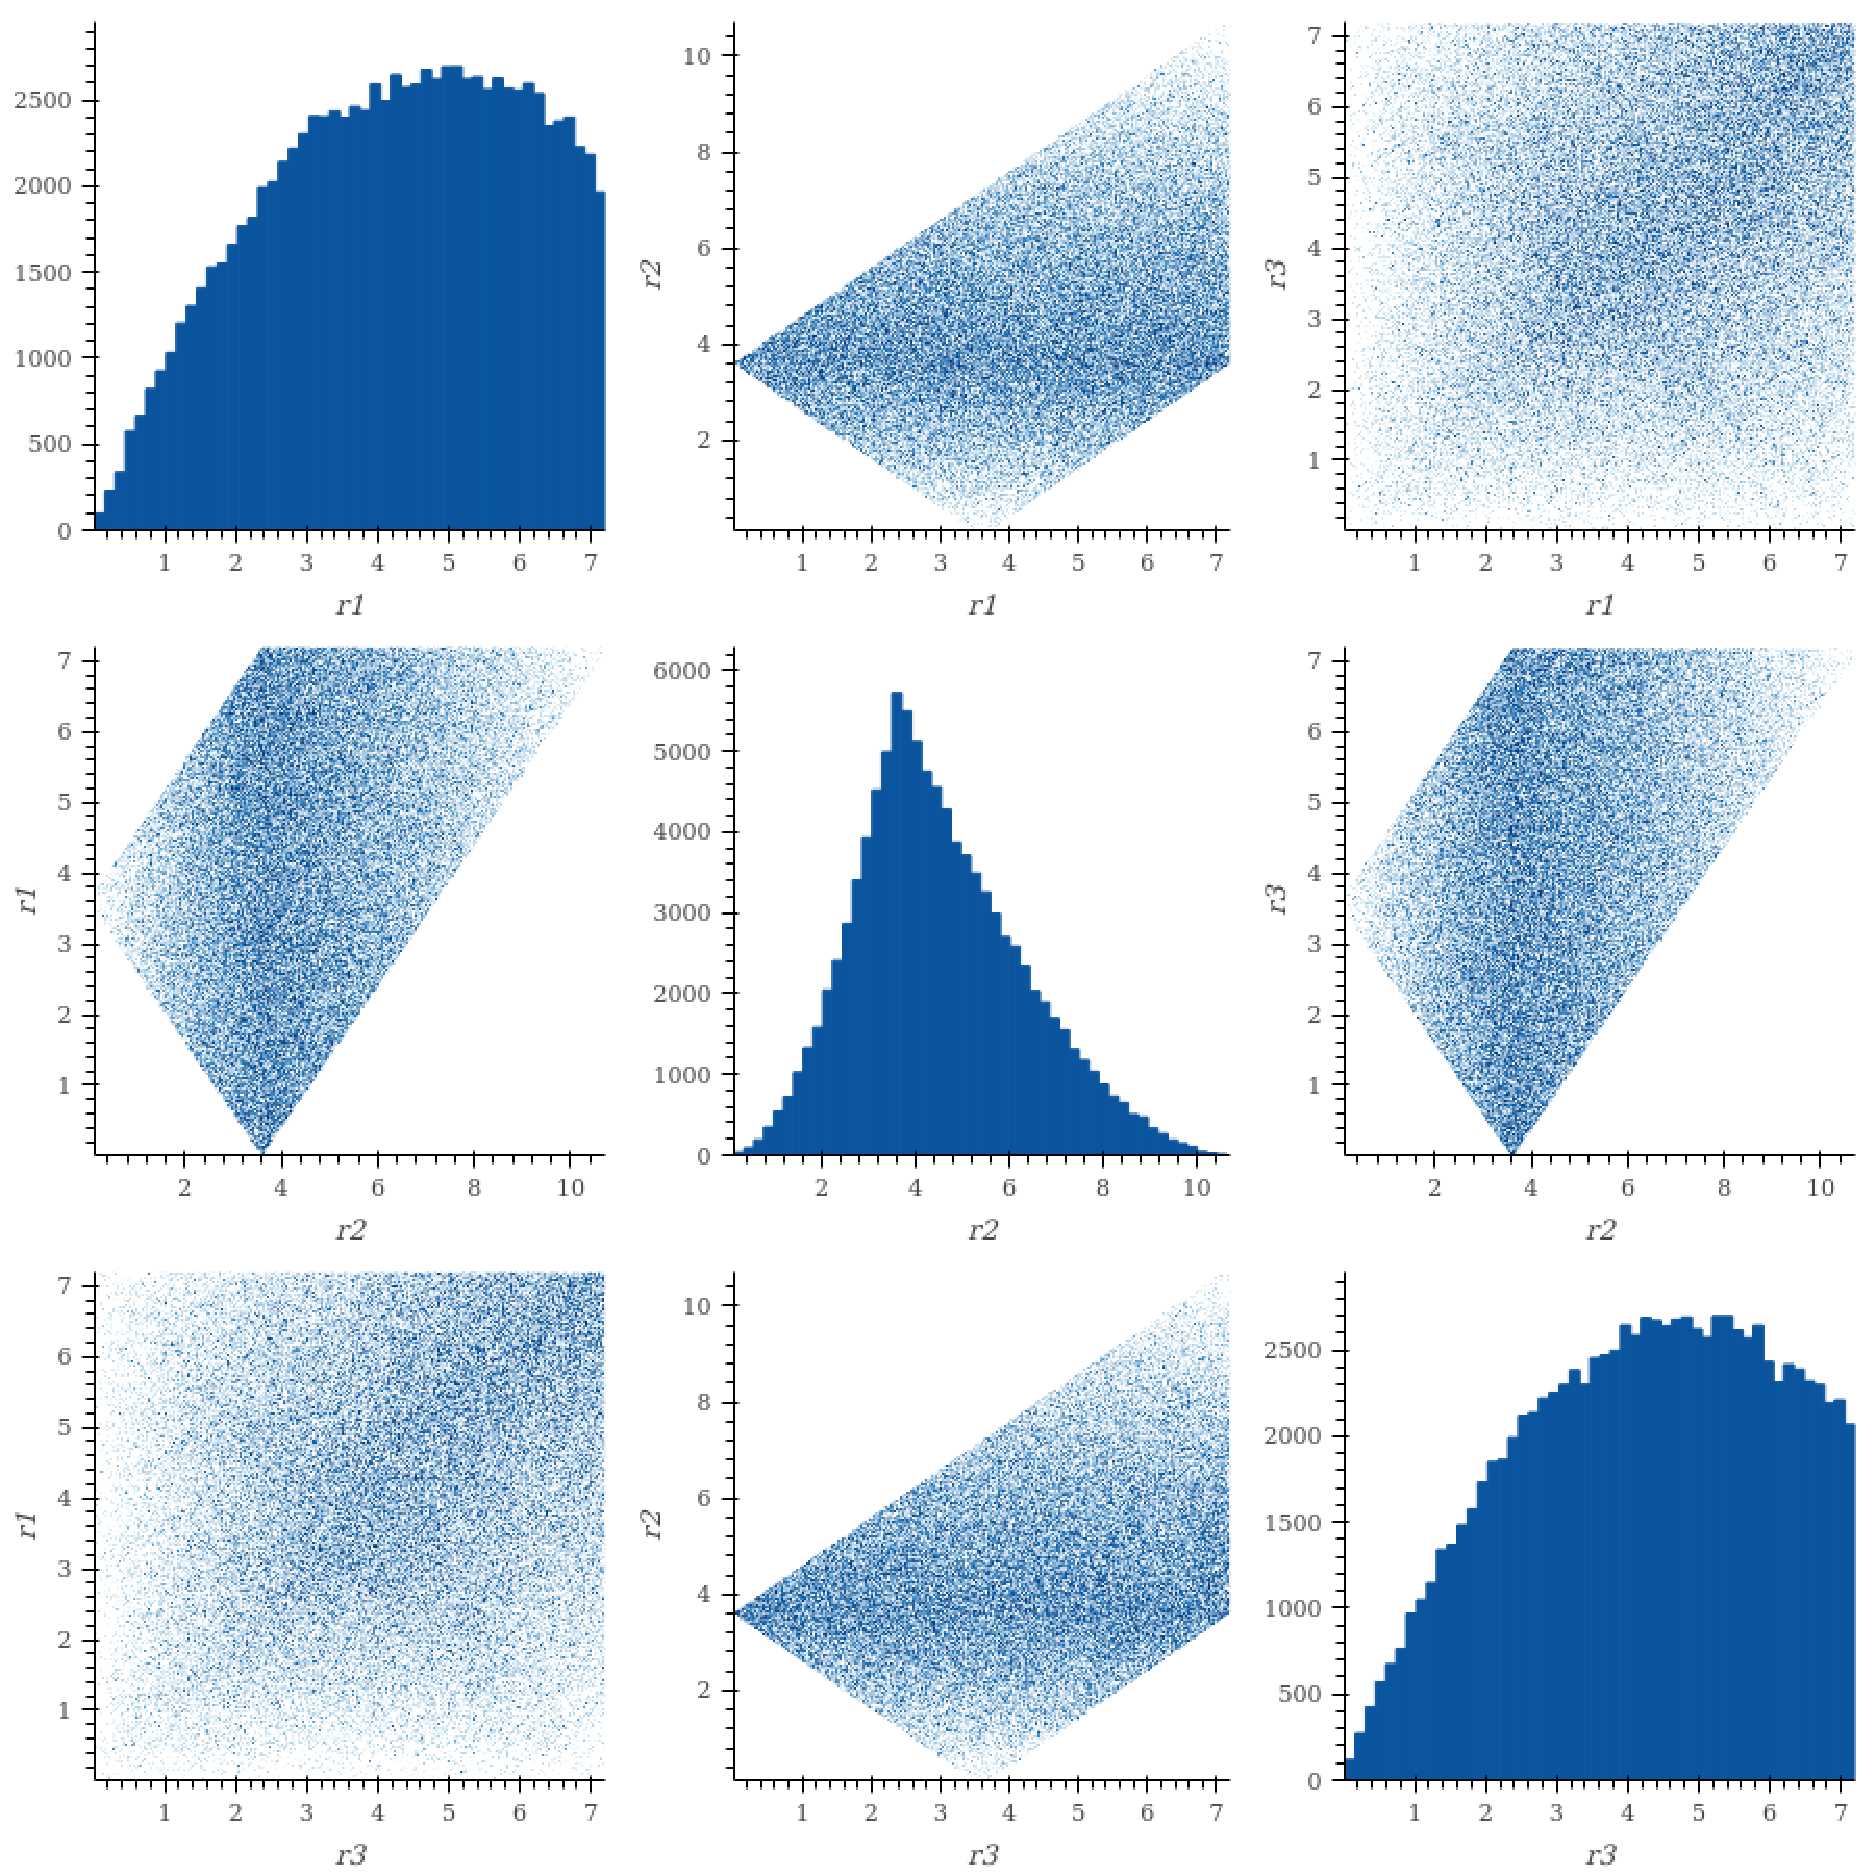
\includegraphics[width=\textwidth]{images/constraind_diffusion_rejection/pairplots/loops_polytope_uniform.pdf}
		\caption{Plots of the univariate marginal and pairwise bivariate distributions of \num{1e5} samples from the uniform distribution in \(\mathbb{P}\subset\R^3\).}
		\label{fig:app_pairplots_loop_polytope_uniform}
	\end{subfigure}
	\hfill
	\begin{subfigure}[t]{0.45\textwidth}
		\centering
		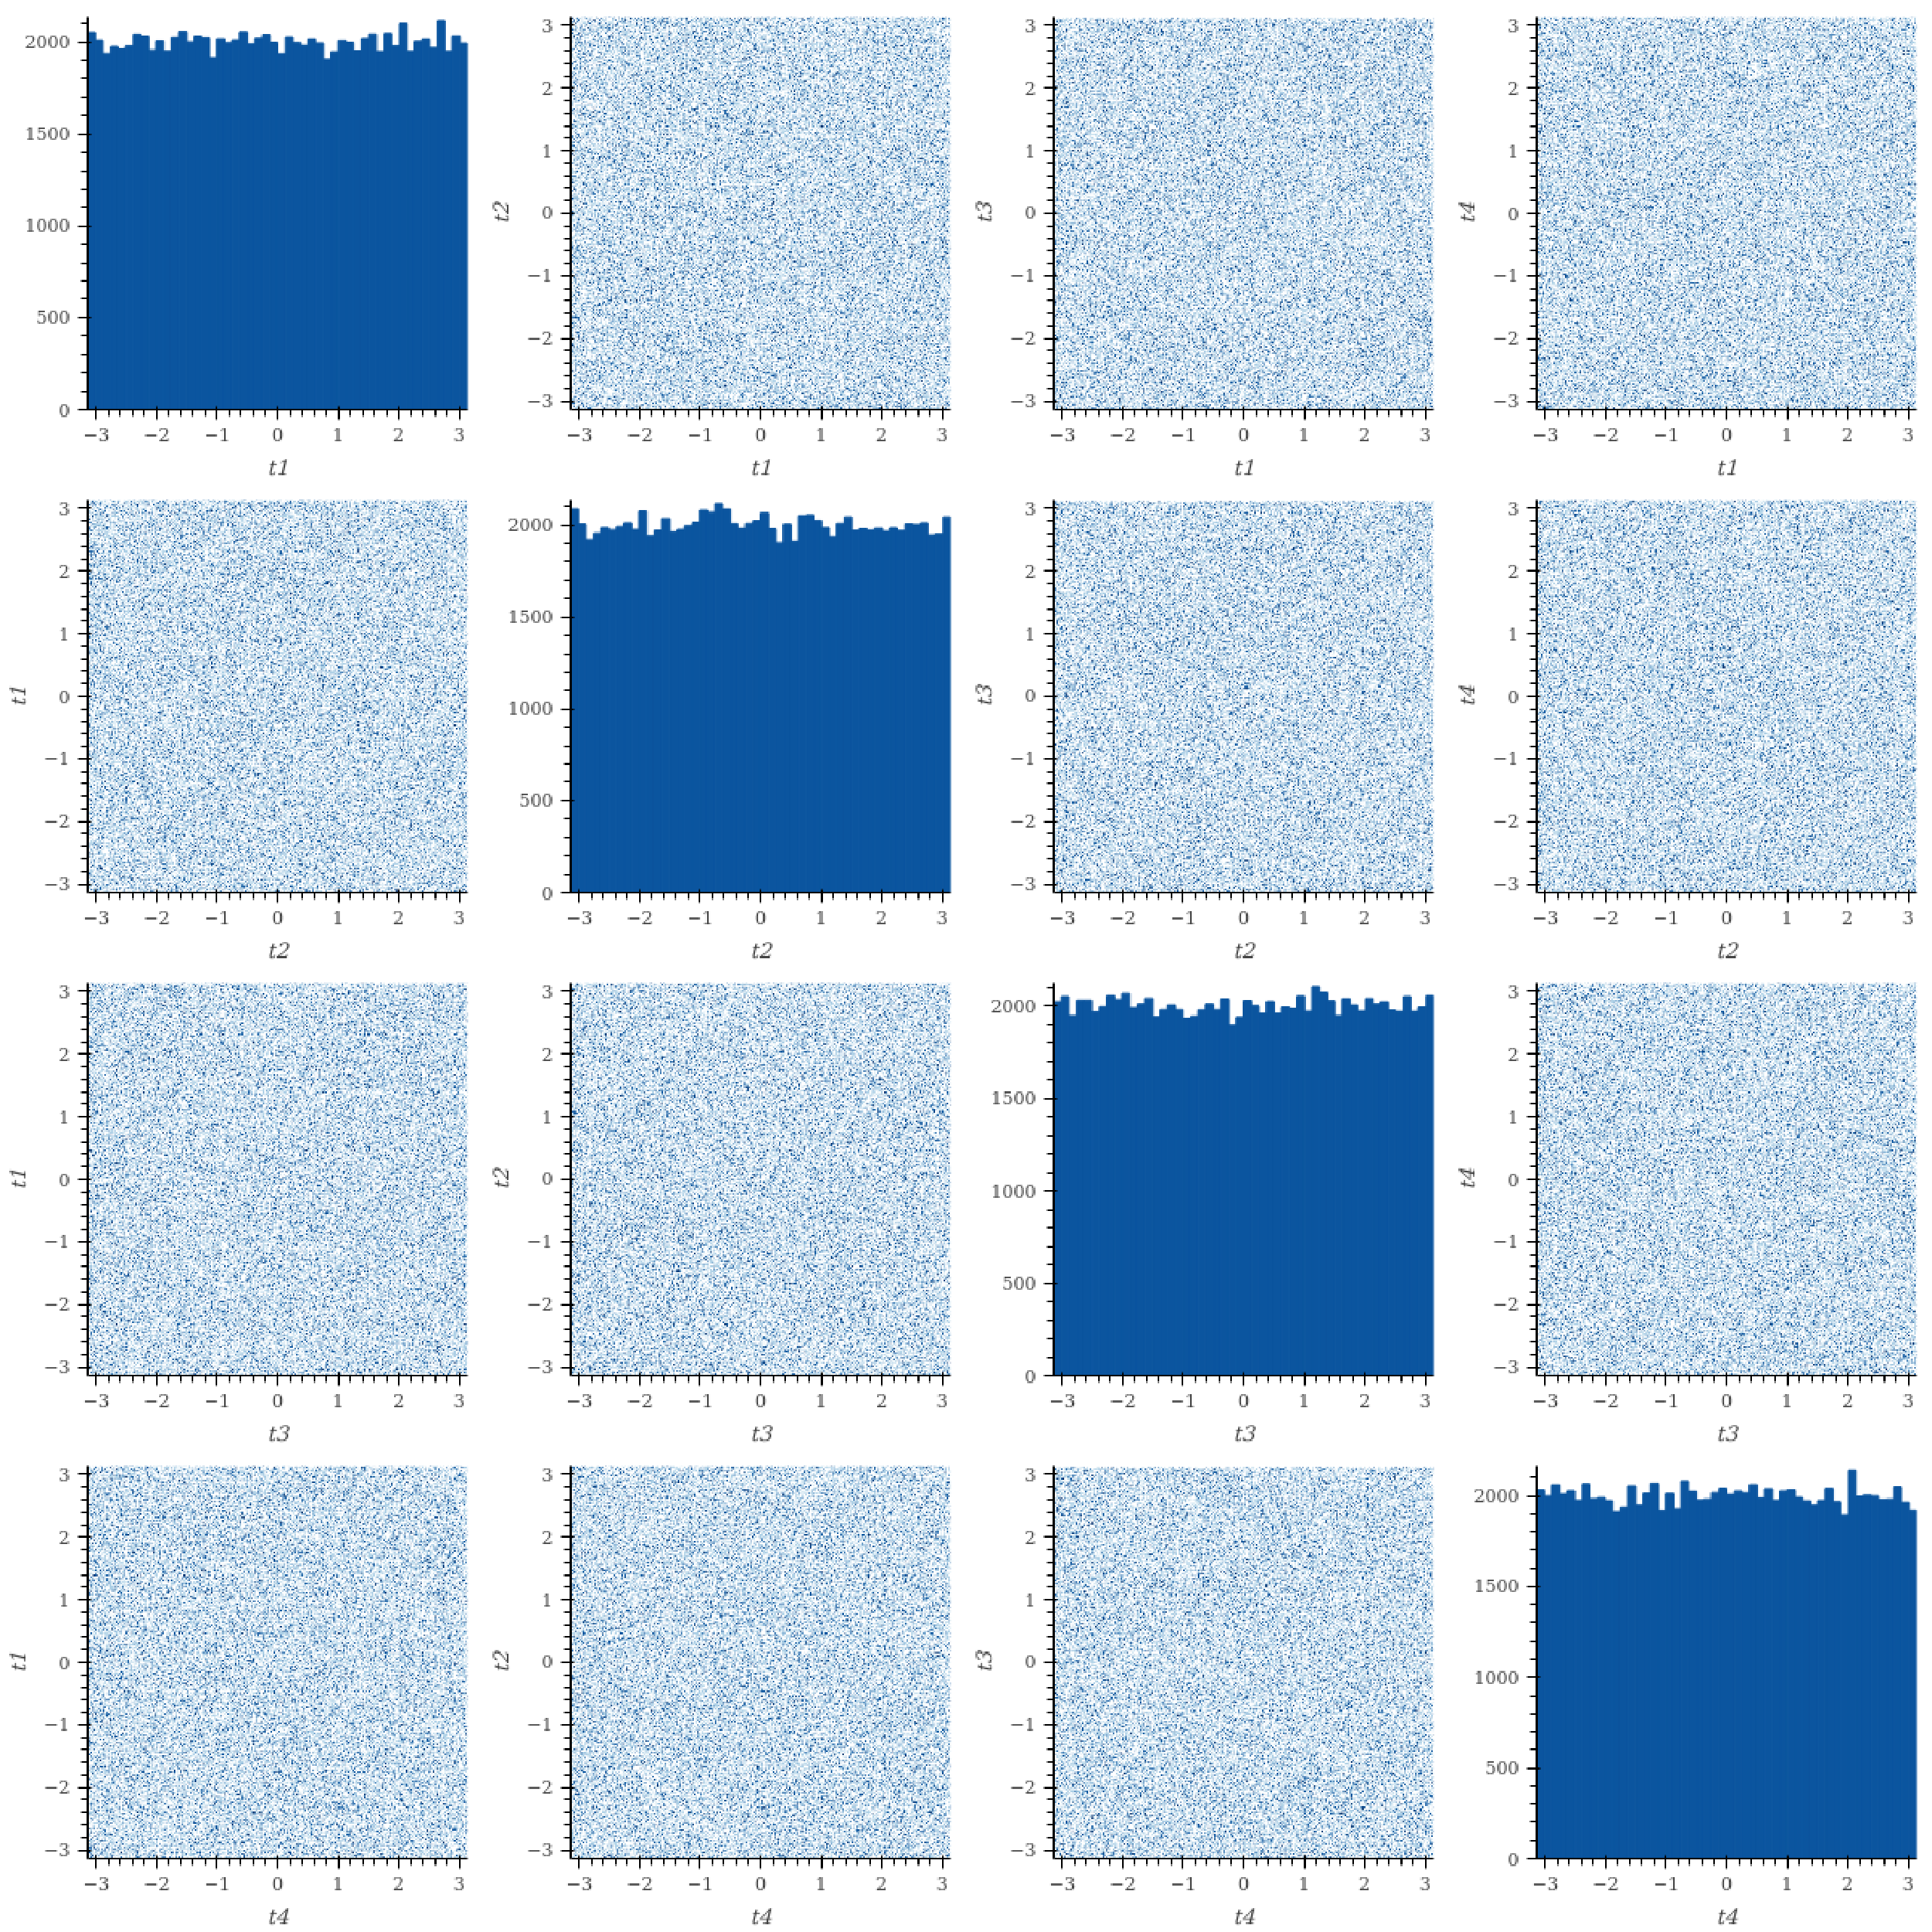
\includegraphics[width=\textwidth]{images/constraind_diffusion_rejection/pairplots/loops_torus_uniform.pdf}
		\caption{Plots of the univariate marginal and pairwise bivariate distributions of \num{1e5} samples from the uniform distribution in \(\mathbb{T}^4\).}
		\label{fig:app_pairplots_loop_torus_uniform}
	\end{subfigure}
	\caption{Visualisation of the uniform distribution in \(\mathbb{P}\subset\R^3\times\mathbb{T}^4\) using univariate marginal and pairwise bivariate plots.}
	\label{fig:app_pairplots_loop_uniform}
\end{figure}
